\definecolor{green}{cmyk}{0,0.25,0.5,0}
\definecolor{orange}{cmyk}{0,0.25,0.5,0}
\newcommand{\weblong}[2]{\href{#1}{#2}} % definition of long hyperreferences
\newcommand {\excl}[1]{
    \begin{tabular}{r p{0.75\textwidth}}
    \hspace*{5mm}\LARGE{\textcolor{green}{$!$
    %\ArrowBoldDownRight
}} & #1\\
\end{tabular}
}
\newcommand {\photo}[3]
{\begin{center}
  \includegraphics[width=0.5\textwidth]{img/#3}
\end{center}}

%%%%%%%%%%%%%%%%%%%%%%%%%%%%%%%%%%%%%%%%%%%%%%%%%%%%%%%%%%%%%%%%%%%%
\ifchinese
\chapter{{\\}基础飞行模拟教程}
\fi
\iffalse
\IfLanguageName{english}{
\chapter{A Basic Flight Simulator Tutorial}
}{}
\fi
\IfLanguageName{french}{
\chapter{Un tutoriel de base de simulation de vol}
}{}
\label{basic}
%%%%%%%%%%%%%%%%%%%%%%%%%%%%%%%%%%%%%%%%%%%%%%%%%%%%%%%%%%%%%%%%%%%%

\ifchinese
\section{序言}
\fi
\iffalse
\IfLanguageName{english}{
\section{Foreword}
}{}
\fi
\IfLanguageName{french}{
\section{Pr\'{e}ambule}
}{}
\label{sec:Foreword}

\ifchinese
航空业充满了各种极端:
\begin{itemize}
\item 飞机非常脆弱却以高速飞行。然而却是最安全的交通工具。
\item 飞行员需要紧跟各种规则和程序。然而飞机却是自由的象征。
\item 只需要很少的一些训练,飞小型飞机是很容易的。然而一旦发生问题,需要在数秒内解决。
\item 很多飞行教程都以幽默的口吻来写,然而若飞行时不够严肃,会让你快速坠地。
\end{itemize}
\fi
\iffalse
\IfLanguageName{english}{
Aviation is about extremes:
\begin{itemize}
    \item An airplane is quite fragile and flies at high speeds.
  Yet it is one of the safest forms of transport.
    \item Pilots must constantly follow rules and procedures.
  Yet an airplane is a symbol of freedom.
    \item With a little training, flight a small aircraft is easy.
  Yet if a problem occurs, you must be able to resolve it in a few seconds.
    \item Many flight tutorials are written with a lot of humor.
  Yet not taking flying seriously will bring you down to earth prematurely.
\end{itemize}
}{}\fi

\IfLanguageName{french}{
L'aviation est faite d'extr\^{e}mes :

\begin{itemize}
    \item Un a\'{e}ronef est assez fragile et vole \`{a} des vitesses \'{e}lev\'{e}es.
  Cependant, c'est l'un des moyens de transports les plus s\^{u}rs.
    \item Les pilotes doivent constamment suivre des r\`{e}gles et des proc\'{e}dures.
  Cependant, un a\'{e}ronef est un symbole de libert\'{e}.
    \item Avec un peu d'entra\^{i}nement, voler un petit a\'{e}ronef est simple.
  Cependant, si un probl\`{e}me survient, vous devez \^{e}tre capable de le r\'{e}soudre en quelques secondes.
    \item De nombreux tutoriels de vols sont \'{e}crits avec beaucoup d'humour.
  Cepedant, ne pas prendre le vol au s\'{e}rieux vous rem\`{e}nera sur le plancher des vaches de mani\`{e}re pr\'{e}matur\'{e}e.
\end{itemize}
}{}

\ifchinese
此教程使用的飞行器是\weblong{http://en.wikipedia.org/wiki/Cessna_172} {塞斯纳 172P} 型。此机型已被用于很多现实中的飞行学校中,并且是一款非常好飞的机型。
\fi
\iffalse
\IfLanguageName{english}{
The aircraft used in this tutorial is the
\weblong{http://en.wikipedia.org/wiki/Cessna_172} {Cessna 172p}. This is the
aircraft used in many real life flight schools and a great airplane to fly.
}{}
\fi

\IfLanguageName{french}{
L'a\'{e}ronef utilis\'{e} dans ce tutoriel est le
\weblong{http://en.wikipedia.org/wiki/Cessna_172} {Cessna 172p}. Il s'agit de l'avion
utilis\'{e} dans de nombreuses v\'{e}ritables \'{e}coles de pilotage et c'est un avions tr\`{e}s agr\'{e}able en vol.
}{}
\medskip
\centerline{
  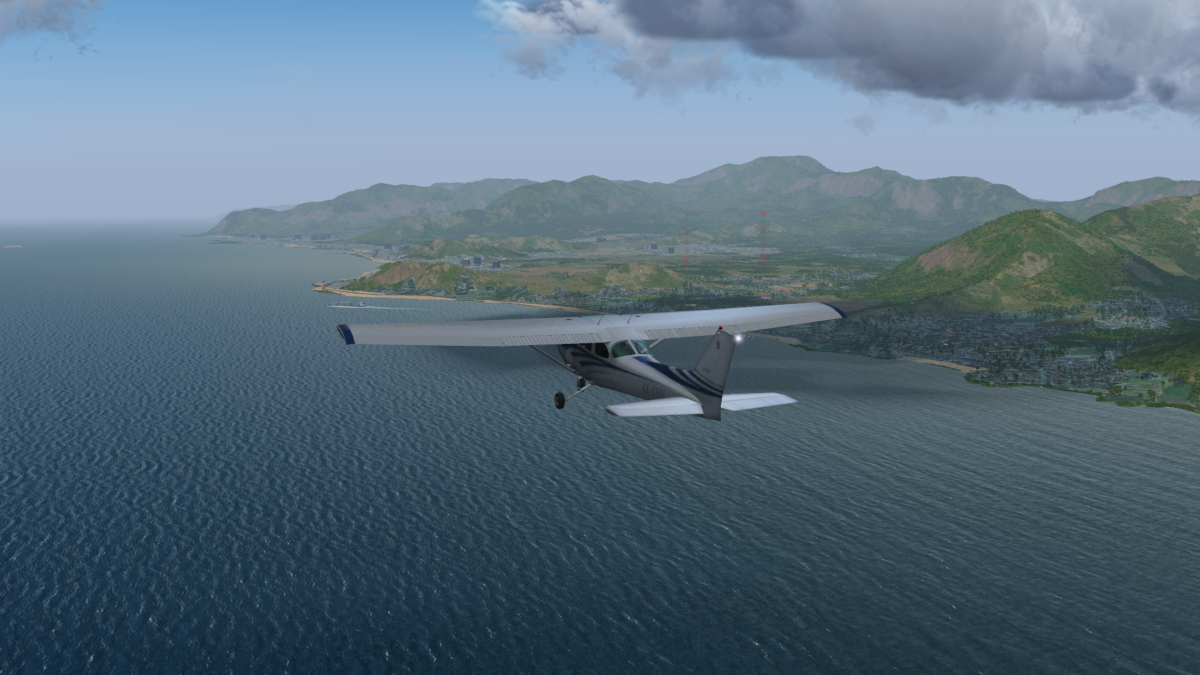
\includegraphics[width=\textwidth]{img/basic_tutorial/sight-seeing}
}
\newpage

\ifchinese
下面的这些文章可以作为此教程的补充,并回答了很多你阅读中的一些问题。特别是第一篇介绍了飞机的主要部件和控制:
\fi
\iffalse
\IfLanguageName{english}{
The following articles complement this tutorial and will answer most questions
that may arise as you read through. The first one in particular is a good
introduction to the airplane's main components and controls:
}{}
\fi
\IfLanguageName{french}{
Les articles suivants compl\`{e}tent ce tutoriel et r\'{e}pondront \`{a} la plupart des questions qui pourraient
survenir lors de votre lecture. Le premier, en particulier, est une bonne
introduction aux principaux composants et contr\^{o}les de l'a\'{e}ronef :
}{}

\begin{itemize}
    \item \weblong{https://www.gleim.com/aviation/learn-to-fly/}    {https://www.gleim.com/aviation/learn-to-fly/}
    \item \weblong{http://www.pilotfriend.com/training/flight\_training/aero/principa.htm}    {http://www.pilotfriend.com/training/flight\_training/aero/principa.htm}
    \item \web{http://en.wikipedia.org/wiki/Aircraft}
    \item \web{https://en.wikipedia.org/wiki/Flight\_control\_surfaces}
    \item \web{http://en.wikipedia.org/wiki/Airplane\_flight\_mechanics}
    \item \web{http://en.wikipedia.org/wiki/Aircraft\_engine\_controls}
    \item \web{http://www.navfltsm.addr.com/}
    \item \web{http://www.free-online-private-pilot-ground-school.com/}
\end{itemize}

\ifchinese
此教程基于我本人的知识,然而不可避免的可能会有一些错误。对此我非常抱歉。
\fi
\iffalse
\IfLanguageName{english}{
This tutorial is accurate to the best of my knowledge, but will inevitably
contain some mistakes. I apologize in advance for these.
}{}
\fi
\IfLanguageName{french}{
Ce tutoriel est pr\'{e}cis dans les limites de mes meilleures connaissances, mais il contiendra in\'{e}vitablement
quelques erreurs. Je m'excuse par avance pour celles-ci.
}{}

\ifchinese
\section{启动}
\fi
\iffalse
\IfLanguageName{english}{
\section{Starting Up}
}{}
\fi
\IfLanguageName{french}{
\section{D\'{e}marrer}
}{}
\ifchinese
根据你的平台和发行版的不同,有很多种方式来启动 \FlightGear{}。不妨回顾一下第 ~\ref{takeoff} 章( ~\nameref{takeoff} )的相关内容。
\fi
\iffalse
\IfLanguageName{english}{
There are a number of different ways to start \FlightGear{} based on your
platform and the distribution you are using.
}{}
\IfLanguageName{french}{
Il existe diff\'{e}rentes mani\`{e}res de d\'{e}marrer \FlightGear{} en fonction de la
plate-forme et de la distribution que vous utilisez.
}{}
\fi
\newpage
\subsection{使用启动器}
\ifchinese
\FlightGear{} 有一个图形化的启动器,让你可以选择机型和起始位置。首先如下图所示在\command{Aircraft}(机型)选项卡里选择 Cessna 172P Skyhawk 飞机。为了能够适应此教程,不要选择 2D 仪表板的版本(你也许会发现 2D 仪表板更适宜培训)。你也可以按\button{返回}(Back)按钮来选择不同的机型。
\fi
\iffalse
\IfLanguageName{english}{
On MS Windows, \FlightGear{} has a GUI Wizard in which you can choose your
aircraft and starting postion. First choose the Cessna 172p airplane as shown
below. To match this tutorial do not choose the 2D panel version.
(You may however find in the future that the 2D version is more appropriate
for training). Click the \button{Next} button to choose your airport.
}{}
\fi
\IfLanguageName{french}{
Sur MS Windows, \FlightGear{} dispose d'un assistant en mode graphique dans
lequel vous pouvez choisir votre a\'{e}ronef et votre position de d\'{e}marrage.
Choisissez d'abord l'a\'{e}ronef Cessna 172p comme montr\'{e} ci-dessous.
Pour correspondre \`{a} ce tutoriel, ne choisissez pas la version avec panneau 2D.
(Vous pourriez cependant trouver dans le futur que la version 2D est plus
appropri\'{e}e pour l'entra\^{i}nement. Cliquez sur le bouton \button{Suivant}
pour choisir votre a\'{e}roport.
}{}

\medskip

\centerline{
  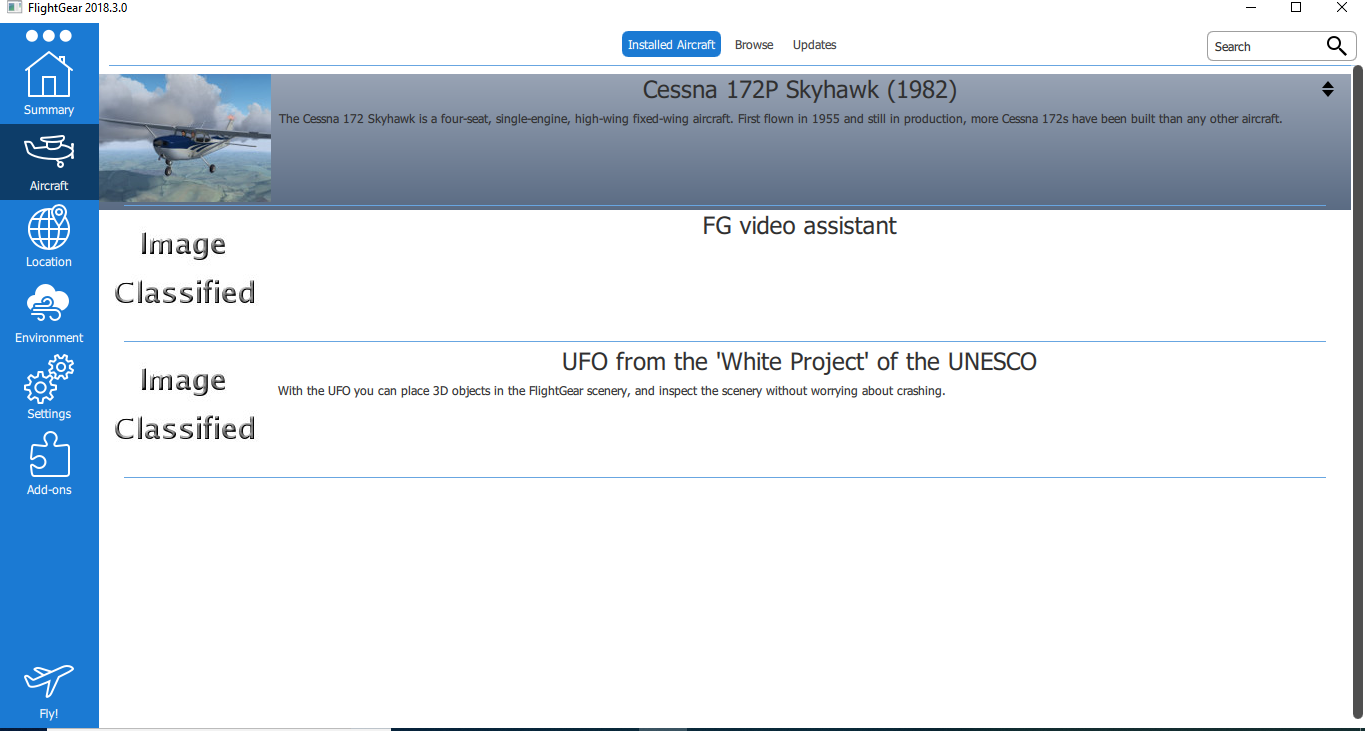
\includegraphics[clip,width=12.5cm]{img/basic_tutorial/launcher-1}
}
\medskip

\ifchinese
你可以从任何机场启动教程,我假设你使用了 FlightGear 默认的檀香山国际机场(PHNL):
\fi
\iffalse
\IfLanguageName{english}{
You can start from any airport for this tutorial, but I will assume that you
will start from FlightGear's default airport of San Francisco (KSFO):
}{}
\fi
\IfLanguageName{french}{
Vous pouvez d\'{e}marrer de n'importe quel a\'{e}roport pour ce tutoriel, mais je partirai
du principe que vous d\'{e}marrerez de l'a\'{e}roport de San Francisco (KSFO), l'a\'{e}roport
par d\'{e}faut de FlightGear :
}{}
\medskip

\centerline{
  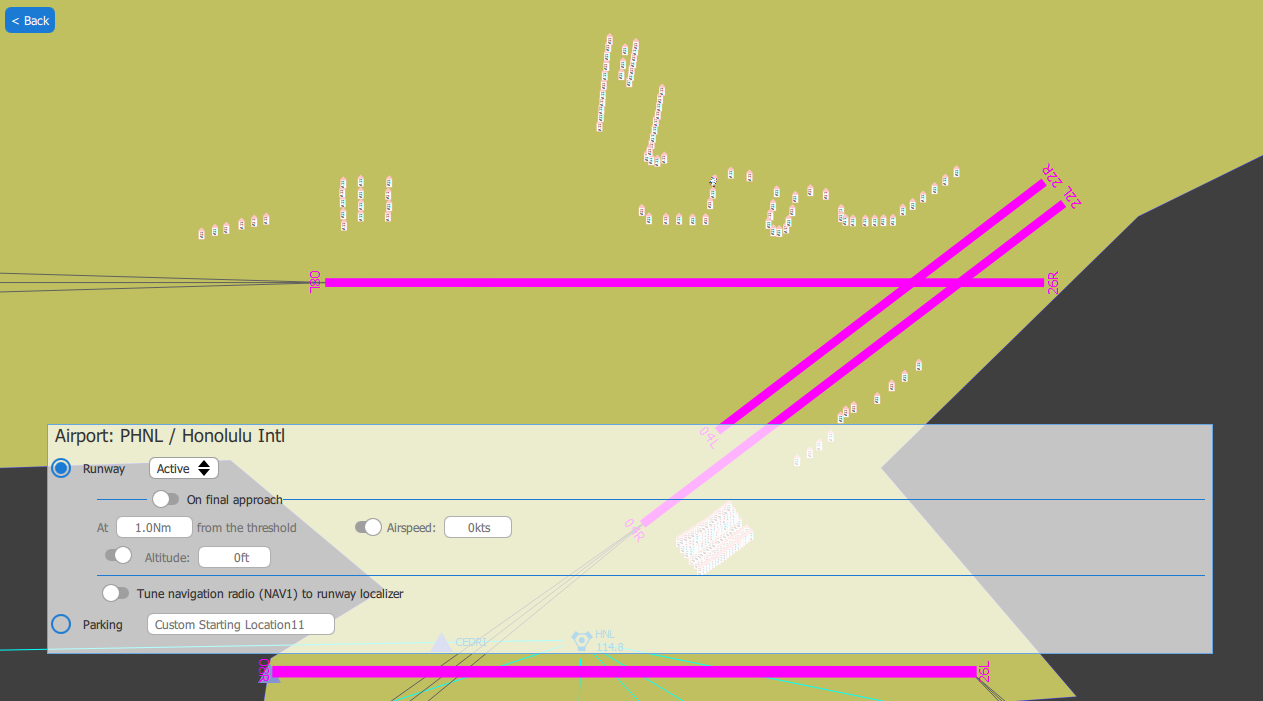
\includegraphics[clip,width=12.5cm]{img/basic_tutorial/launcher-2}
}
\newpage

\ifchinese
在 Location(位置)选项卡选择好了 PHNL 之后还可以点\button{返回}按钮选择其他位置。对模拟器来说你可以从任何时间点起飞,不过对于你的第一次飞行,我建议设置在正午时间,可以从 Environment(环境)选项卡里选择。
\fi
\iffalse
\IfLanguageName{english}{
Once you have selected KSFO and clicked on the \button{Next} button, you can set
any number of options for the simulator. For your first flight, I suggest
starting at noon. I would also recommend that you start with a small resolution
of $800\times600$. Later on, you can play around with the options and use a
higher resolution, but this obviously adversly affects performance. Click on the
\button{Run} button and \FlightGear{} will start with the options you
selected.
}{}
\fi
\IfLanguageName{french}{
une fois que vous avez choisi KSFO et cliqu\'{e} sur le bouton \button{Suivant}, vous pourrez
param\'{e}trer toutes les options que vous souhaitez pour le simulateur.
Pour votre premier vol, je vous sugg\`{e}re de d\'{e}marrer \`{a} l'heure
de midi. Je recommanderais \'{e}galement de d\'{e}buter avec une petite
r\'{e}solution de $800\times600$. Par la suite, vous pourrez vous amuser avec les
options et utiliser une meilleure r\'{e}solution, cependant ceci affecte la performance de
mani\`{e}re n\'{e}gative. Cliquez sur le bouton \button{D\'{e}marrer} et \FlightGear{} d\'{e}marrera avec les options que vous avez
choisi.
}{}
\medskip

\centerline{
  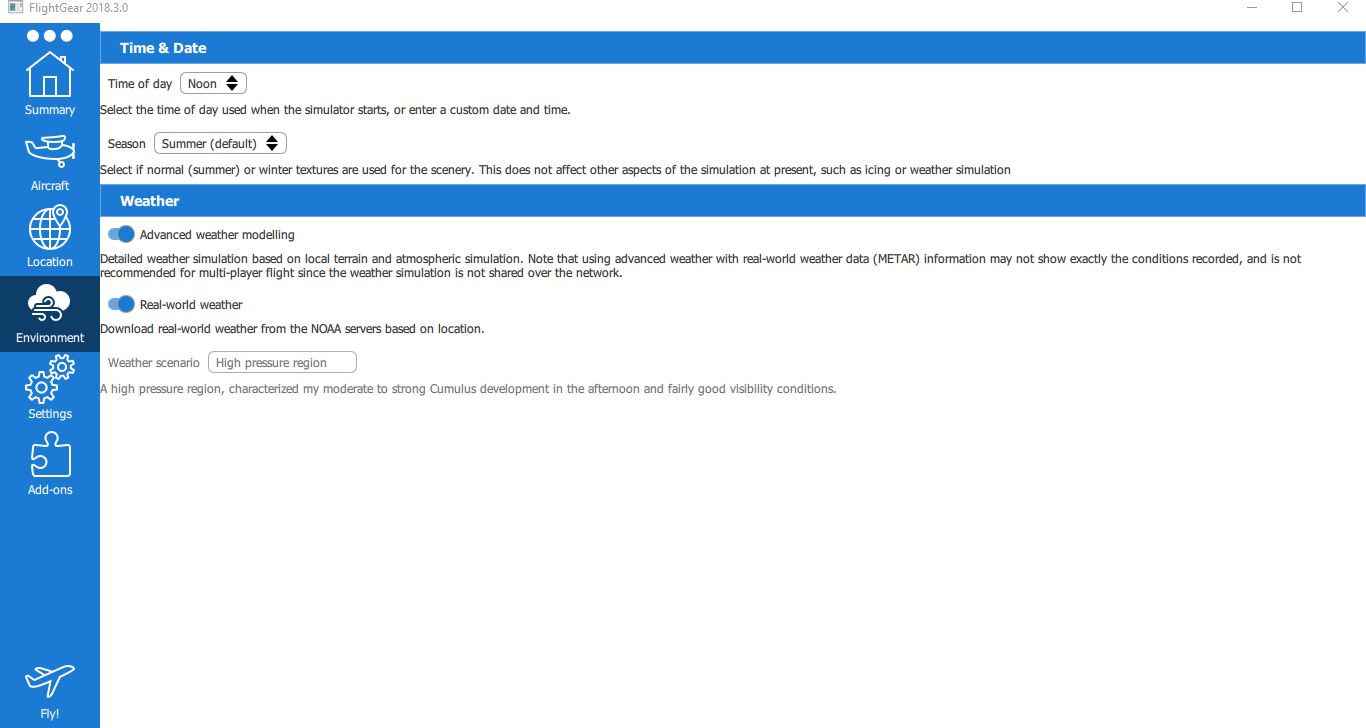
\includegraphics[clip,width=12.5cm]{img/basic_tutorial/launcher-3}
}
\medskip
\ifchinese
另外建议你使用小一点的分辨率 $800\times600$。你可以从\command{Settings}(设置)选项卡的\command{View and Window}(视觉和窗口)一栏旁边点开\button{Show More}(显示更多)按钮就可以修改分辨率设置了。之后你可以再使用更高的分辨率,然而这对性能会有较大影响。按\button{Fly!}(开始飞行)按钮,则会应用你的选项来启动 \FlightGear{}。
\fi

\medskip

\centerline{
  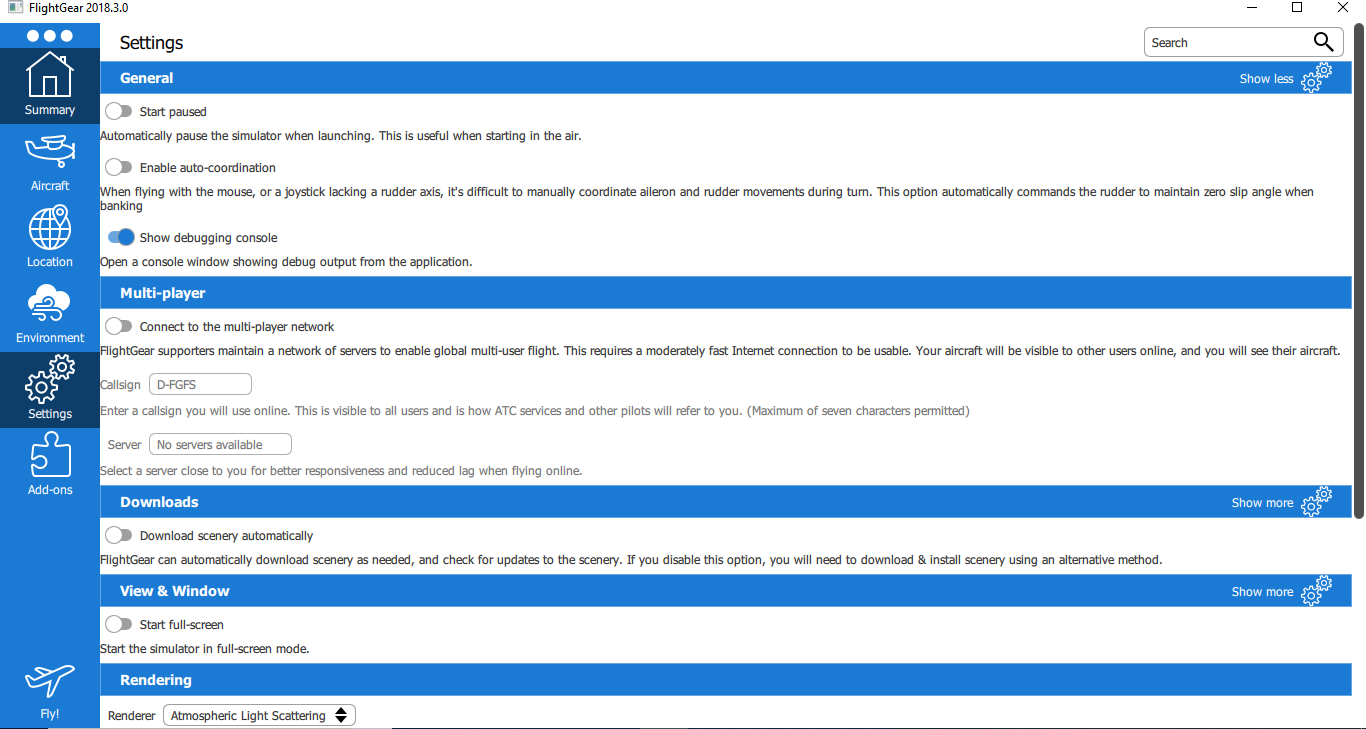
\includegraphics[clip,width=12.5cm]{img/basic_tutorial/launcher-4}
}
\medskip

\ifchinese
如果你运行最新版的 \FlightGear{} 有问题的话,可以尝试使用较旧的版本这样可以减低对显卡的需求。你可从 \FlightGear{} 下载页面找到 FTP 镜像来下载:\\ \web{http://www.flightgear.org/download/}。
\fi
\iffalse
\IfLanguageName{english}{
If you have problems running the latest version \FlightGear{} on
your Windows system, you may want to try an earlier version with lower
graphics requirements (for example 0.9.8). You can find previous releases on
the FTP mirrors mentioned at the top of the \FlightGear{} download page:
\weblong{http://www.flightgear.org/download/}.
}{}
\fi
\IfLanguageName{french}{
Si vous rencontrez des difficult\'{e}s \`{a} faire fonctionner la derni\`{e}re version de
\FlightGear{} sur votre syst\`{e}me Windows, vous pourriez tender d'essayer une version
avec des pr\'{e}-requis moindres en mati\`{e}re de graphisme (comme par exemple la
0.9.8). Vous pouvez trouver les version pr\'{e}c\'{e}dentes sur les miroirs FTP
mentionn\'{e}s en haut de la page de t\'{e}l\'{e}chargement de \FlightGear{} :
\weblong{http://www.flightgear.org/download/}.
}{}

\IfLanguageName{english}{
If you are running under Windows Me and the flight simulator suddenly starts
\index{troubles!stuttered simulation}stuttering, with the frame rate dropping,
try killing all tasks except Explorer and Systray before you
launch \FlightGear{}. If one of the tasks you kill is an antivirus or
such protection software, this is an obvious security risk. Also, on one
Windows Me machine, a \FlightGear{} of $800\times600$ yielded good results,
while a lower resolution of $640\times480$ triggered much lower FPS levels
(Frames Per Second).)
}{}
\fi

\IfLanguageName{french}{
Si vous fonctionnez sous Windows Me et que le simulateur commence soudainement
\`{a} \index{probl\`{e}mes!simulation saccad\'{e}e}saccader, avec un taux d'image
par seconde qui diminue, essayez de stopper toutes les t\^{a}ches de fond de
votre syst\`{e}me mis \`{a} part Explorer et Systray avant de lancer \FlightGear{}.
Si l'une des t\^{a}ches que vous supprimez est un antivirus ou un autre logiciel de
protection, c'est un risque de s\'{e}curit\'{e} \'{e}vident. Aussi, sur une machine
Windows Me machine, un \FlightGear{} de $800\times600$ a donn\'{e} de bons
r\'{e}sultats, alors qu'une r\'{e}solution inf\'{e}rieure de $640\times480$ donne
des niveaux de taux de d'image par seconde (FPS, Frames Per Second) bien inf\'{e}rieurs.
}{}

\newpage

%%%%%%%%%%%%%%%%%%%%%%%%%%%%%%%% CHINESE VERSION %%%%%%%%%%%%%%%%%%%%%%%%%%%%%%%%%%%%%%%%%%%%%%

\ifchinese
\section{第一个挑战——直线平飞}\label{sec:FlyingStraight}

当 \FlightGear{} 启动以后,你的第一个任务是起动发动机。可以通过菜单\command{Cessna C172P -> Autostart}非常容易的起动发动机。
\medskip

\centerline{
  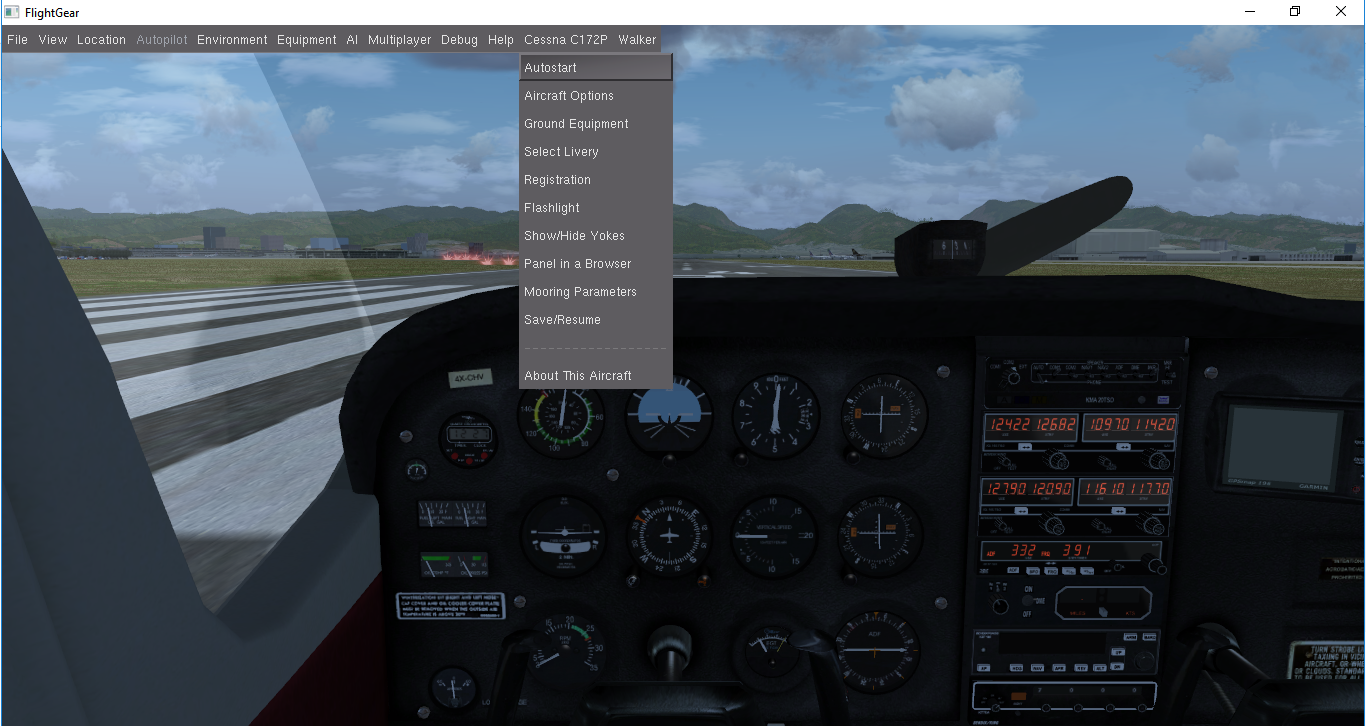
\includegraphics[clip,width=15.0cm]{img/basic_tutorial/autostart}
}
\medskip

启动时,飞机停在跑道的起点且发动机维持低功率运转。飞机也许会轻微抖动,但不会移动。

\medskip

\centerline{
  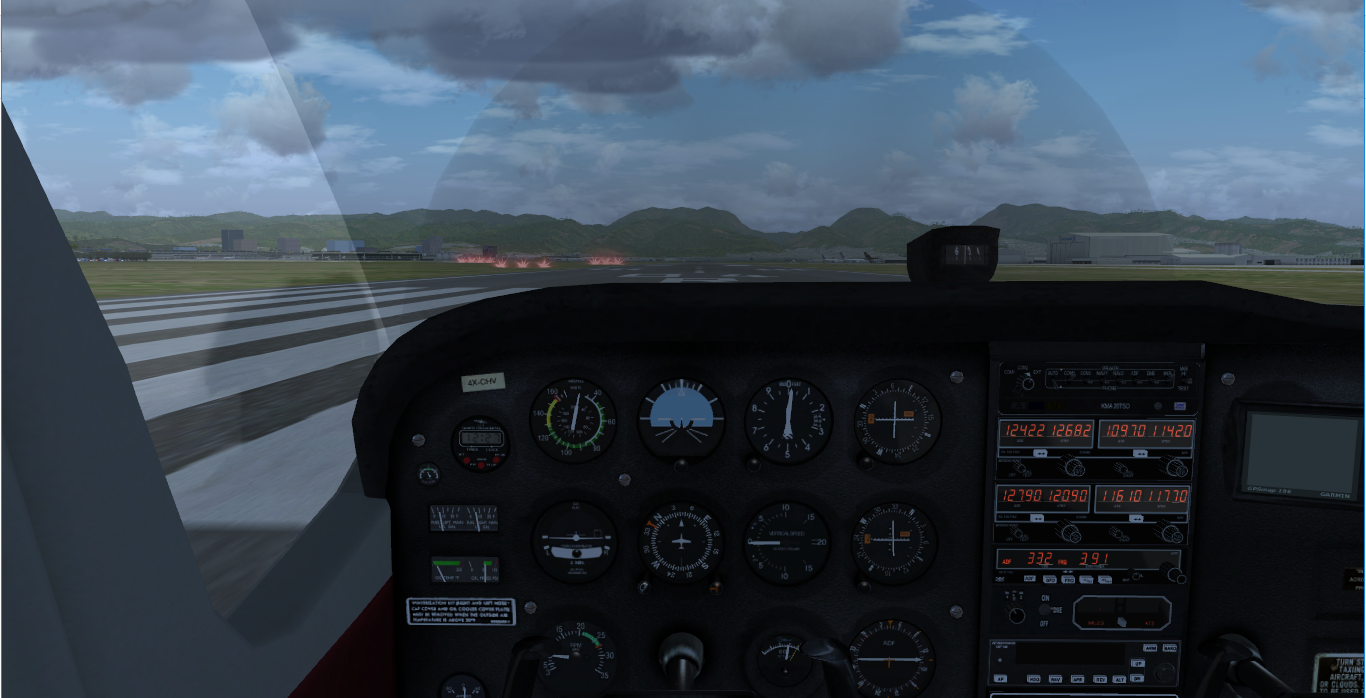
\includegraphics[clip,width=15.0cm]{img/basic_tutorial/on-runway}
}
\medskip

\subsection*{关于键盘控制}\index{键盘}

\begin{itemize}
    \item 在本教程中,小写字母表示你只需要按这个键即可,大写意味着你需要同时按 \textcolor{blue}{\key{$\Uparrow$~Shift}} 键和这个键。也就是说,如果你看到“v”键表示你只需要按字母 \key{v} 即可,如果你看到“V”则意味着你需要按下 \key{Shift} 键的同时按字母 \key{v}\index{键盘!大写和小写键}(简单来说, V 就代表\key{Shift-v})。
    \item 本教程假设你的 \key{NumLock} 是已经打开的状态。键盘右上角的绿灯亮起。如果没亮,按\textcolor{green}{\key{NumLock}}键直到绿灯亮起。
\end{itemize}
\medskip

\centerline{
  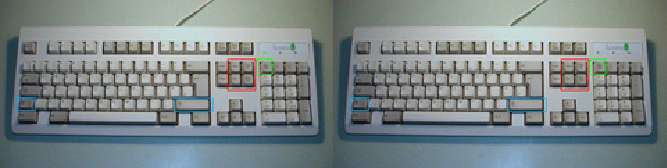
\includegraphics[width=0.95\textwidth]{img/basic_tutorial/numlock}
}
\medskip
\index{视图!改变}

按 \key{v} 键来从外面查看飞行器。重复按 v 键可以循环各种视图模式,直到你回到驾驶舱中。按 \key{V} 将会反向循环。按 \key{Ctrl-v} 会回到驾驶舱视图:

\medskip

\centerline{
  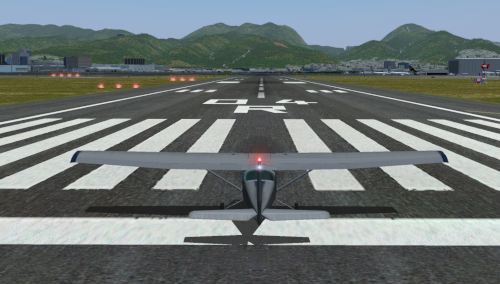
\includegraphics[clip,width=7.0cm,height=4.0cm]{img/basic_tutorial/extern1}
  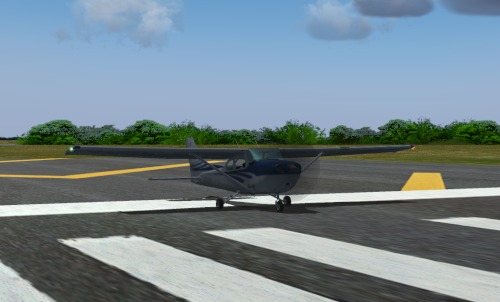
\includegraphics[clip,width=7.0cm,height=4.0cm]{img/basic_tutorial/extern2}
}
\medskip

现实中,我们会围着飞机转一圈检查所有都正常,没有任何东西阻碍移动控制面,也没任何物体堵住仪表的输入口。而在模拟器里,这些都已经在启动前帮我们做好了。

按住 \key{Page Up}(或小键盘的数字 9 键) 大概八秒,你能听到发动机的声音越来越大。 

飞机开始在跑道上加速。在离地之前,飞机会被拉向左侧,并向左侧倾斜,并坠毁在地面上(也许)。

\index{视图!即时回放}

你可以通过 \button{View -> Instant Replay} 来检查整个坠毁过程的回放。按对话框底部的 \button{Replay} 按钮,下面这张图就是坠毁时的状态。你按 \key{F3} 可以截图保存。你可以用 \key{F10} 来切换菜单是不是显示。
\medskip

\centerline{
  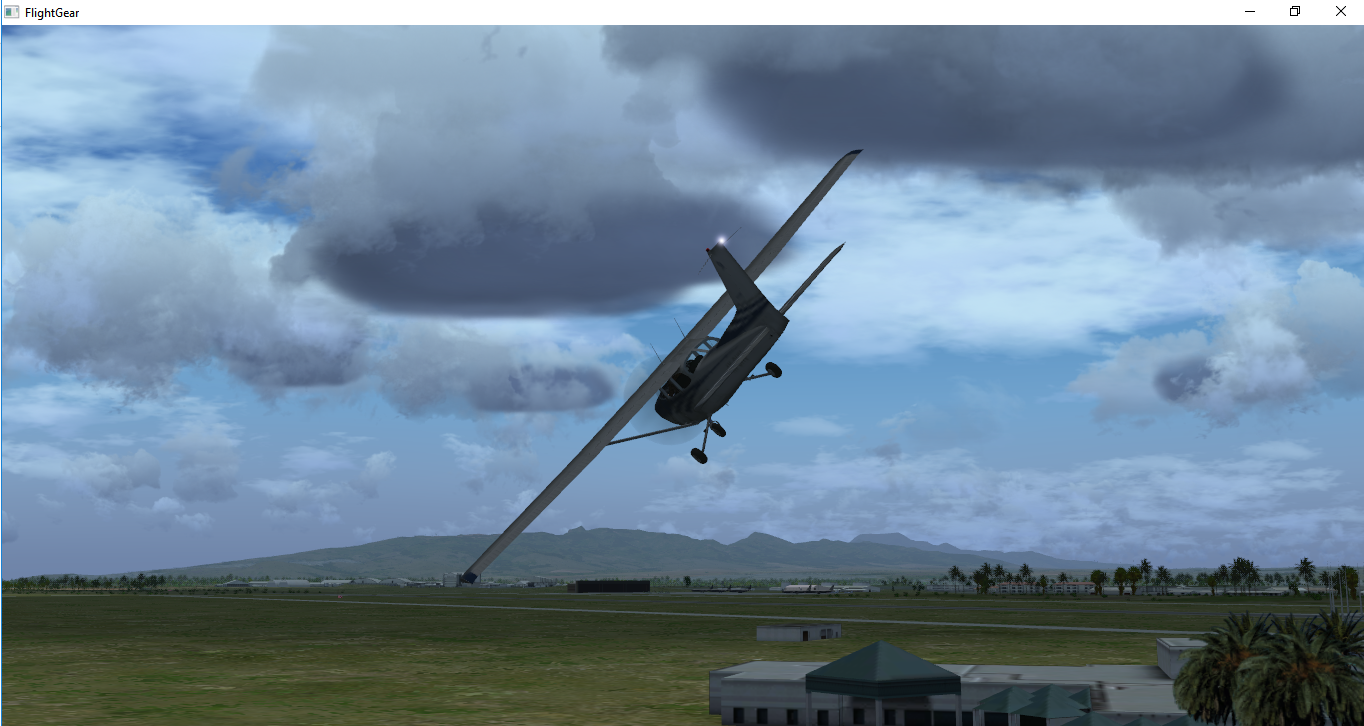
\includegraphics[width=0.5\textwidth]{img/basic_tutorial/crash}
  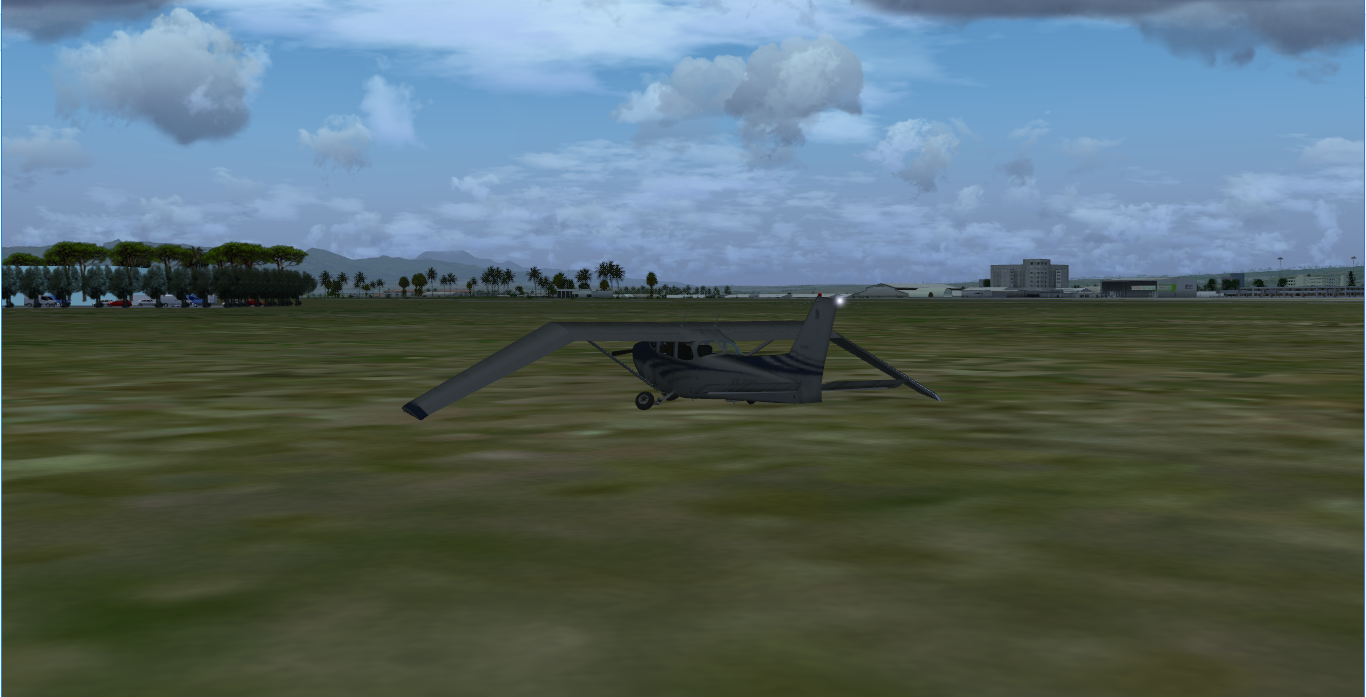
\includegraphics[width=0.5\textwidth]{img/basic_tutorial/crash-plunged-to-ground}
}
\medskip

看过坠机之后,你可以用 \button{File -> Reset} 重置 \FlightGear{} 回到坠机之前的状态。

为了能够直线飞行,我们需要控制飞机的\Index{驾驶盘}:
\medskip

\centerline{
  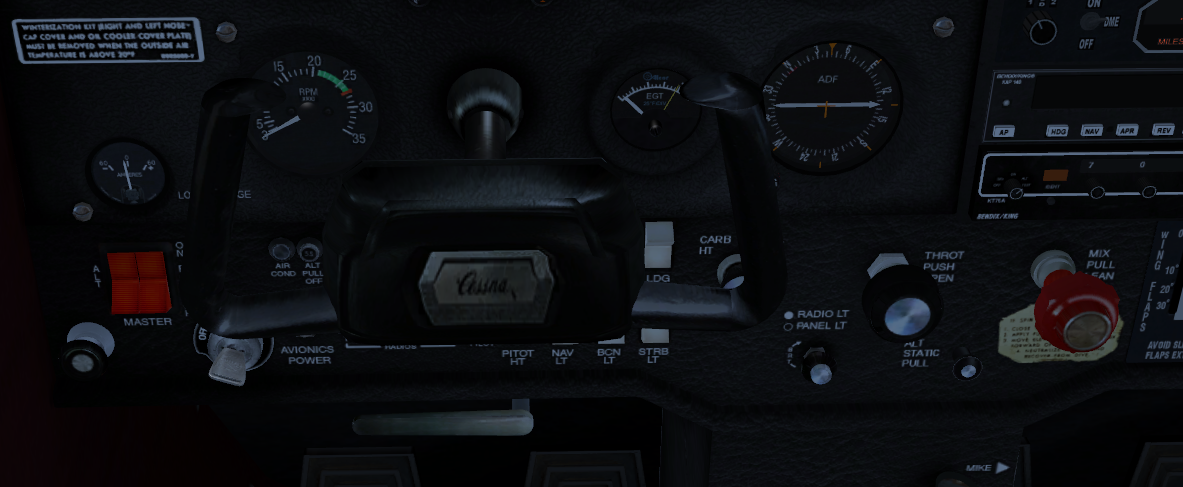
\includegraphics[width=\textwidth]{img/basic_tutorial/yoke}
}
\medskip

你可以用游戏杆或者鼠标来控制。要使用鼠标你需要将鼠标置于控制模式,可以通过按 \key{Tab} 键直到指针变成 $+$ 形。移动鼠标就可以看到驾驶盘也在随之移动。按 \key{v} 键可以从外面观察飞机。此时继续移动鼠标,可以看到机尾的升降舵和机翼后部的副翼也在移动。如果你的视点离飞机太远,看不清楚的话,可以按几次 \key{x} 键来放大,按 \key{X} 来缩小。\key{Ctrl-x} 可以恢复默认的缩放级别。此时按 \key{Ctrl-v} 回到驾驶舱里。

按 \key{Tab} 几次直到鼠标进入查看模式。在此模式下,鼠标指针会变成 $\leftrightarrow$ 形。这可以让你更容易的移动鼠标环顾四周。按鼠标左键将会重新回到中间。你可以在控制模式临时进入观察模式,只需要按住鼠标右键并移动鼠标。最后再按 \key{Tab} 会回到正常鼠标模式。

简单来说,\key{Tab} 让鼠标在三个模式之间循环:
\begin{itemize}
    \item \textit{正常模式}\index{鼠标!正常模式}。此模式让你可以点击菜单或点击仪表板。
    \item \textit{控制模式}\index{鼠标!飞行控制模式}\index{驾驶盘!飞行控制模式}。 此时鼠标控制驾驶盘(指针是 $+$ 形)。
    \item \textit{查看模式}\index{鼠标!查看模式}。此时鼠标控制观察的角度(指针是 $\leftrightarrow$ 形)。
\end{itemize}

现在尝试在起飞,按 \key{Tab} 进入飞行控制模式,用鼠标控制驾驶盘。按住 \key{PageUp} 键将发动机油门推到最大功率,不要强制通过鼠标让其在跑道上保持直线,就让它这样向左滑行直到自己升入空中。然后用鼠标尝试让飞机保持直线平飞。(如果你想控制在地面的飞机,请查看 \ref{sec:TaxiTurning} 小节)。

你会发现你需要防止飞机向左滚转……或者向右滚转::

\medskip

\centerline{
  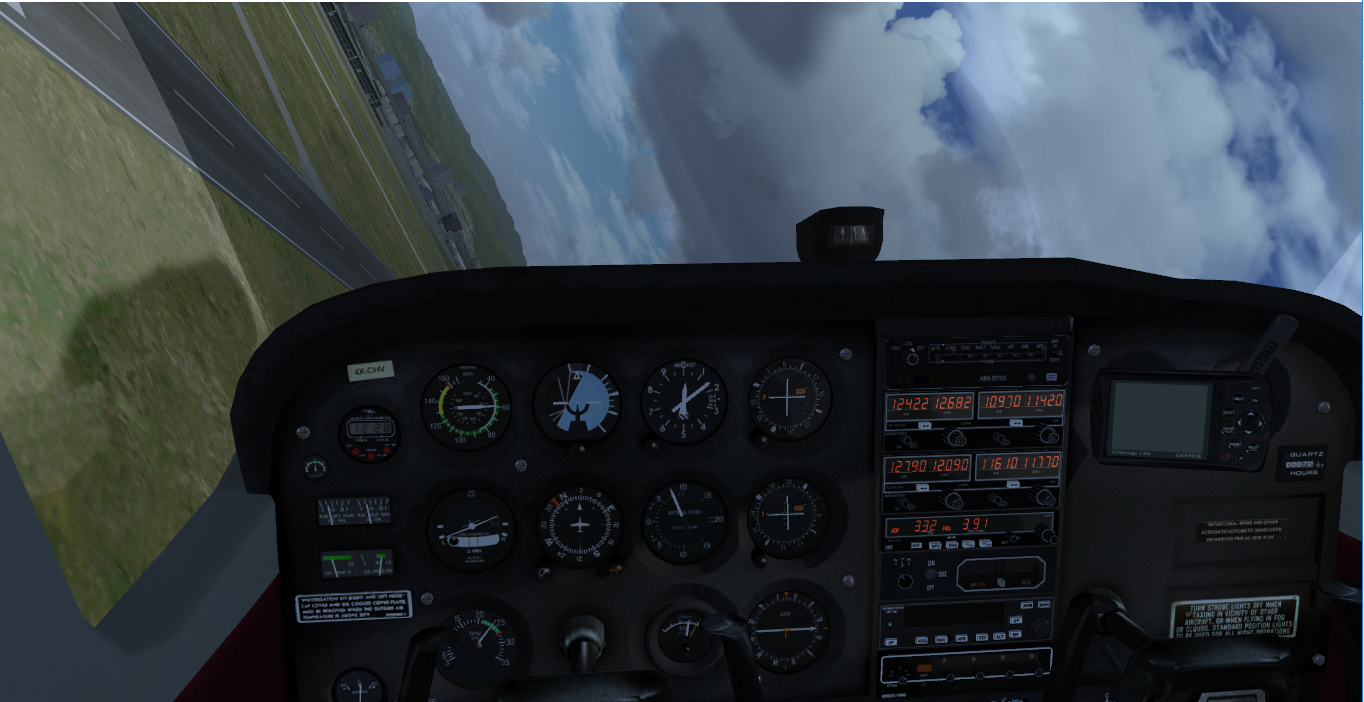
\includegraphics[width=0.5\textwidth]{img/basic_tutorial/bank-left}
  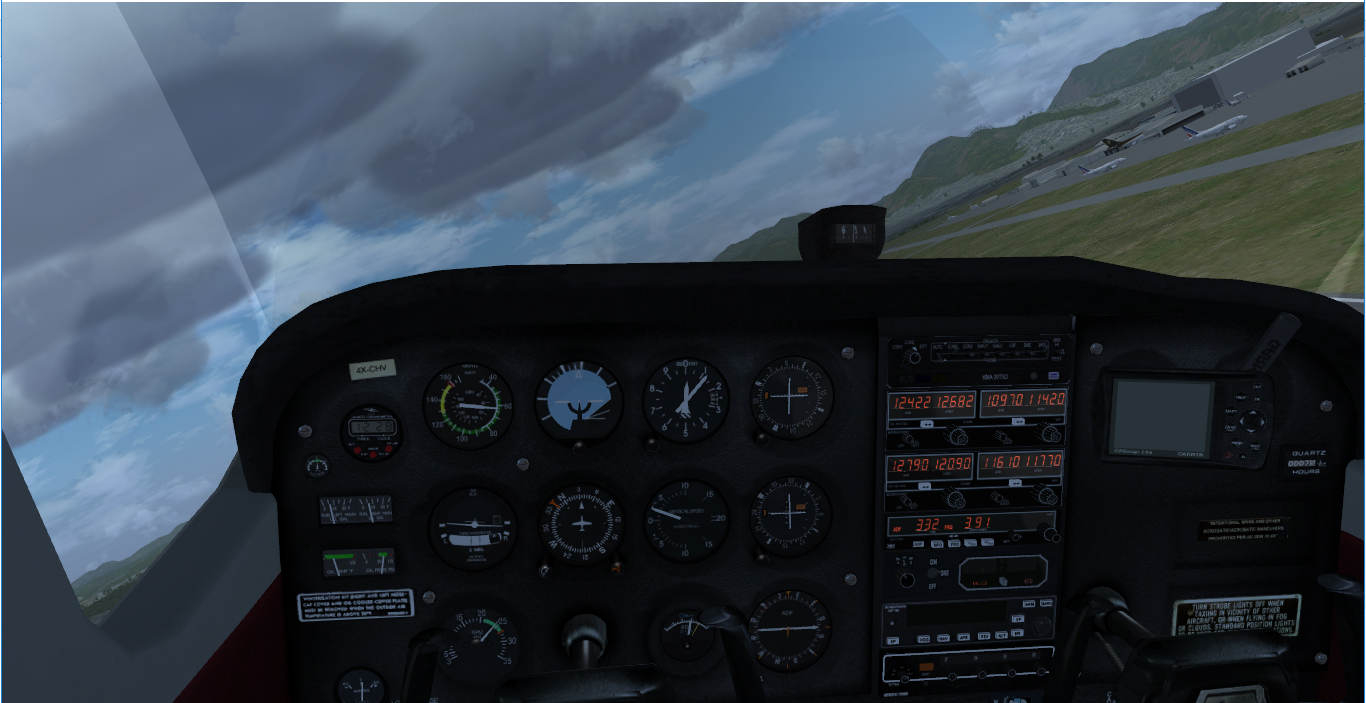
\includegraphics[width=0.5\textwidth]{img/basic_tutorial/bank-right}
}
\medskip

……或者一头向地面扎去:

\medskip

\centerline{
  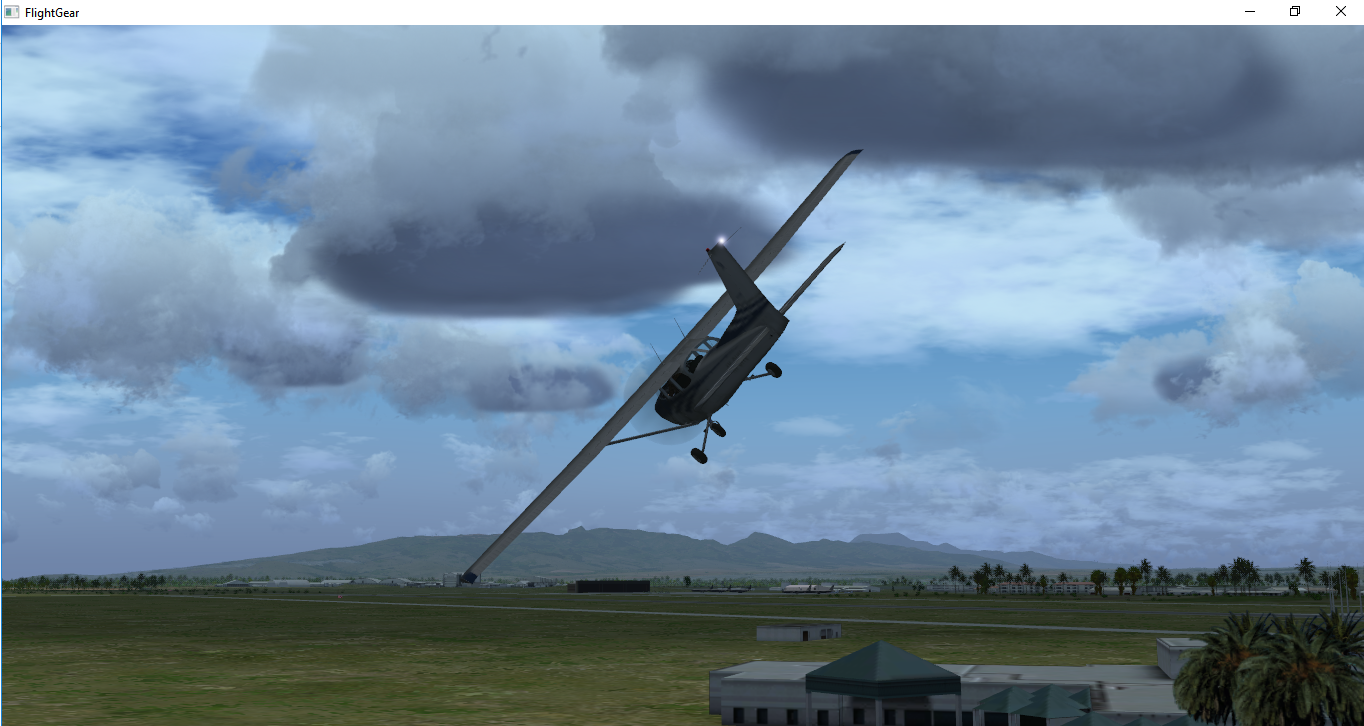
\includegraphics[width=0.5\textwidth]{img/basic_tutorial/crash}
}
\medskip

尽可能的沿直线飞行,让地平线稍稍高于机头:
\medskip

\centerline{
  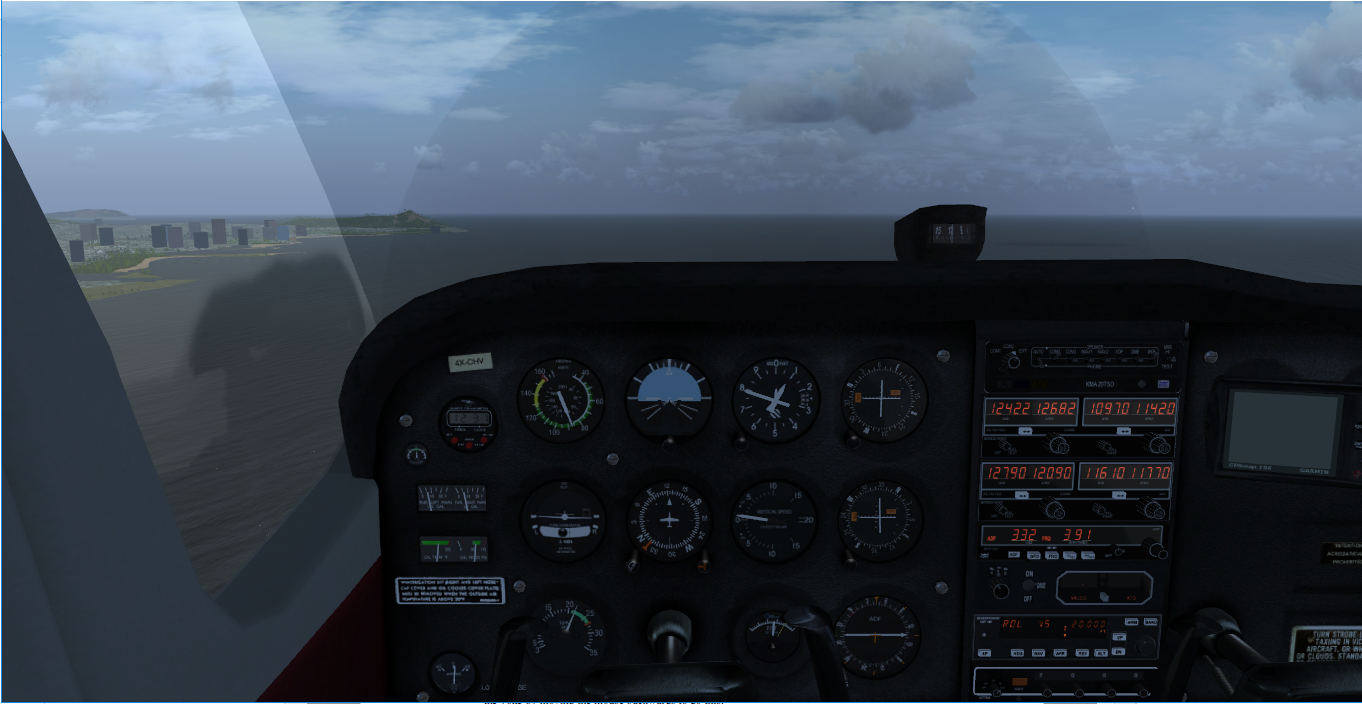
\includegraphics[width=\textwidth]{img/basic_tutorial/straight-level}
}
\medskip

无论你在电脑游戏或模拟游戏方面的能力如何,第一次飞行很可能不会成功。飞机可能会坠毁,也许只在起飞后不久。这也就是为什么很多人对真实性比较高的飞行模拟感到绝望。只需要多多尝试,也许你会找到一种很舒适的控制方式。

\subsection*{常见错误}\index{常见错误}

\index{驾驶盘!拉杆}
最常出现的错误是移动太多鼠标,导致飞机的运动失控。或者向前移动鼠标,以使机头向上昂起。
\medskip

驾驶盘的小幅移动就可以对飞机的运动产生很大的影响。尝试放松下来仅小幅移动驾驶盘。如果你发现飞机的反应太微妙,你也可以随时增加一些控制输入。相反地,大幅的驾驶盘移动可以导致飞机很剧烈的反应,这样你会需要拼命重新找回控制感。如果你发现很难控制,还可以在刚开始训练的时候尝试降低鼠标的敏感度。\index{问题!鼠标速度}

记住,\command{拉杆}机头会向上抬起\command{推杆}机头会向下。你需要向后移动鼠标以向后拉驾驶盘抬起机头。同样地,当你想要机头向下,就必须向前移动鼠标。也许这有些奇怪,不过所有飞机都是按照这种方式来控制的。随着时间的推移,你会明白这种方式的好处。

如果你需要更形象的比喻,这么说也许会一些帮助:假设在你桌子上有一个美式橄榄球,而你的手必须“粘在”球的顶端。如果你要向前移动,则球就会向前滚动,而你的手指则会碰到桌面。如果你向后移动手指,则球会向后滚动,而你的手指就会指向天花板。你的手就是飞机。

另一个普遍的错误是假设驾驶盘的动作与飞机的滚转坡度一致。也就是说,你认为只要驾驶盘水平,飞机也会平飞。事实并非如此,驾驶盘只是控制飞机滚转的\emph{速率}。如果飞机有向左 20\textdegree{} 的坡度,而驾驶盘是水平的,则意味着飞机会保持向左 20\textdegree{} 的坡度直到外力改变这个状况。如果想要让飞机恢复平飞,需要温柔的向右转动驾驶盘(温柔的向右移动鼠标),并稍稍维持向右一段时间。飞机会向右慢慢滚转。当与地平线平齐时,再将驾驶盘慢慢转平。飞机会保持平飞(直到外力来改变其方位)。

还有一个错误是尝试找到驾驶盘/鼠标的“正确位置”。很自然的,你想找到一个完美的位置,可以让飞机保持直线平飞。事实上没有这种理想的驾驶盘位置。飞机在空中的运动本质上是不稳定的,你需要不断的用鼠标做小幅移动,来修正飞机的姿态并保持直飞。也许刚开始会让你耗费全部注意力。这就如同开车,让飞机保持直线平飞将很快会变成一种本能。对长期的飞行来说,你还可以偶尔使用自动驾驶仪来保持平飞,不过本教程将不会涉及。

为了帮助你找到控制的感觉,眼睛始终关注着窗外景物,而不要叮着驾驶盘或仪表板。检查地平线与机头之间的位置,地平线和你飞机的发动机盖子是你的主要仪表。只是每隔一段时间扫一眼仪表板而已。

在鼠标处于控制模式时\index{驾驶盘!鼠标控制模式},千万不要将鼠标移出 FlightGear 窗口边缘以外。一旦鼠标离开窗口,就会停止控制飞机,很可能会造成极糟糕的动作!如果你想在窗口外使用鼠标,首先按 \key{Tab} 键两次切换到正常模式。

你也可以使用键盘上的 \key{方向键} 来控制驾驶盘,或者使用小键盘上的 \key{8}、\key{2}、\key{4} 和 \key{6} 键。也许最开始这种方式会比鼠标控制来的简单一些,飞行时的微调控制却不如鼠标,因此持续练习鼠标控制才是王道。

也许你在机场附近飞行时,会听到蜂鸣器的声音,这是降落辅助信号\index{降落!辅助信号}。现在不用担心这些声音。

你会想知道在掌握了这些以会如何爬升。下一步要学习如何维持高度,或者在你的控制下缓慢上升和下降。

让飞机保持一个高度需要观察高度表,并通过前后小幅移动鼠标来让飞机停止上升或下降。

\index{高度表 Altimeter}高度表位于仪表板的中上部,长表针表示百英尺,短表针表示千英尺。下面这张图里的高度表示意的是 800 英尺,约 245 米\footnote{1 英尺 = 12 英寸 = 0.3048 米。口算时可以简单将英尺数除以 3,即得公制米数。——译者注}。

\medskip

\centerline{
  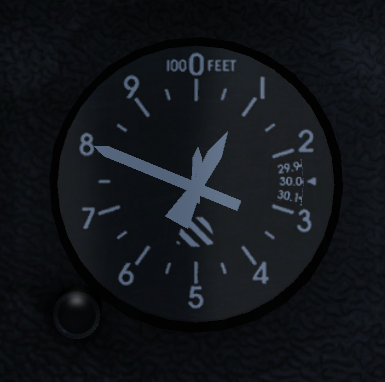
\includegraphics[width=0.5\textwidth]{img/basic_tutorial/altimeter}
  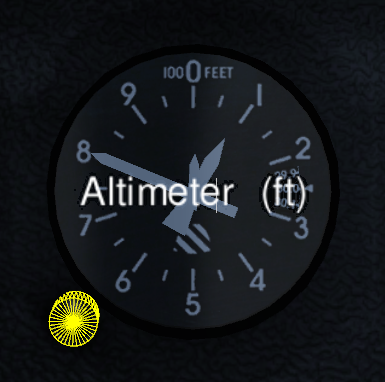
\includegraphics[width=0.5\textwidth]{img/basic_tutorial/altimeter-hotspot}
}
\medskip

上升或下降时高度表会作出反映,表针逆时针转表示下降,顺时针表示高度增加。如果你看到高度表“狂转”,说明你在快速掉高度,缓慢向后移动鼠标拉起机头即可。

一段时间以后你会发现,当平飞的时候,机头与地平线的相对位置永远是一样的。这就是平飞时的飞机姿态。让机头处在这个位置,你就几乎可以让飞机进入平飞而不需要参考任何仪表。这样你就可以微调高度了。

谨记:高度表不会自动显示距海平面的绝对高度\index{高度!绝对高度}。你需要调整其与当地的气压相匹配。高度表左下角的黑色旋钮让你可以调整高度表拨正值\index{高度表!拨正值}。启动 \FlightGear{} 以后一直待在地面上,点击(鼠标在正常模式)这个黑色的旋钮,点击左侧可以让旋钮数值变小,点击右侧则会变大。使用这个小旋钮调整到当前高度。前提是你能获得当前真实的高度。例如你在 1100 英尺,那么就调整旋钮,让高度表显示 1100 英尺。使用鼠标中键点击可以让旋钮旋转更快,或者你可以用鼠标滚轮。\key{Ctrl}-\key{c} 可以将可点击的区域高亮化。

为了更简便的设置高度表,机场会将其修正海平面气压通过各种方式告知出来。也许会通过无线电服务(美国称之为 ATIS\footnote{ATIS 是 Automatic Terminal Information Service 的缩写,意为”自动终端情报服务“,中国大陆称为“情报通播”。机场在一个单独的无线电频率上广播,包括主要的与飞行相关的信息,如天气、可用跑道、气压及高度表拨正值等信息。——译者注,摘自中文维基百科})广播当前的修正海平面气压。单位是英尺汞柱(inHg)。高度表上有一套齿轮组,高度表会利用拨正值来计算高度,你可以通过旋钮设置高度表拨正值\footnote{除美洲外,修正海平面气压的单位在欧洲和亚洲一般使用的是百帕(hPa)为单位。标准大气压是 1013.25 百帕,也就是 29.92 英尺汞柱。1 inHg = 33.86 hPa。设置高度表拨正值时,一般忽略小数点。——译者注}。另外,如果你在地面上已经知道当前机场的标高(相对海平面的高度),你也可以直接调节高度表直到其显示正确的高度。

注意,知道“距地面高度”和“距海平面高度”这两个概念的差异是非常重要的。如果你以距平均海平面高度(Above Mean Sea Level,AMSL)24000 英尺(约 7315 米),飞行在珠穆朗玛峰附近,你距地面(Above Ground Level,AGL)的垂直距离会小很多。因此了解自己距离周边地面的垂直距离,显然很有帮助\footnote{为了分清“距离地面”还是“距离平均海平面”,常会用“高”(Height)和“高度”(Altitude)来区别。本手册的翻译也遵循此规律。——译者注}。

\section{基本转弯}
\label{sec:InFlightTurning}
\begin{wrapfigure}{r}{0.35\textwidth}
  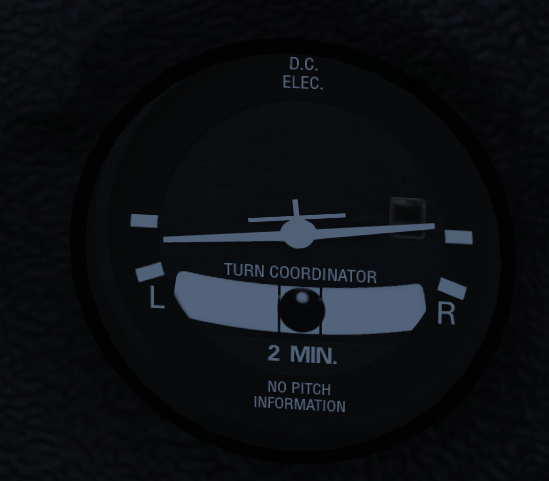
\includegraphics[width=0.35\textwidth]{img/basic_tutorial/turn-coordinator}\index{转弯协调仪}
\end{wrapfigure}
当然,如果你有足够的燃料,你可以直线飞数千英里返回同一机场,能够改变方向将使您的飞行更加愉快和有用。

当你可以或多或少的学会直线平飞以后,让我们来开始学习转弯。原理非常简单:
\begin{itemize}
    \item 当飞机向左滚转时,就会向左转弯
    \item 当飞机向右滚转时,就会向右转弯
\end{itemize}

如果想很好的转弯,不需要很大的坡度,20\textdegree{} 就已经足够并可以安全而稳定的转弯了。更何况大坡度也会让乘客感觉心惊肉跳。

\medskip

\noindent\fbox{转弯协调仪\emph{不能}反映飞机的坡度}
\medskip

\footnote{对好奇的飞行员,你可能很想知道不同的真空速(TAS)下,标准的 3\textdegree{} 转弯率所对应的转弯坡度是多少。
  你可以用这个公式大致计算:
  \[ angle \approx \frac{TAS (knots)}{10} + 7 \]
  \smallskip
  \centerline{
    \begin{tabular}{| c | c | c |}
      \hline
      TAS(节)& 公式 & 转弯坡度 \\
      \hline
      80  & 8 + 7 & 15\textdegree{} \\
      100 & 10 + 7 & 17\textdegree{} \\
      120 & 12 + 7 & 19\textdegree{} \\
      \hline
    \end{tabular}
  }
}

转弯协调仪表示转弯速率。标准转弯率是每秒 3\textdegree{}。为什么这很重要?坦白讲这会救你的命!如果你在低能见度下失去空间定向能力,最聪明的做法是做一个 180\textdegree{} 转弯。在低能见度下,你怎么知道自己已经转了半圈?那么标准转弯速率就能帮到你。如果你做一个每秒 3\textdegree{}的标准转弯,那么转半圈正好是一分钟。两分钟以后则会转一个完整的圆。这也就解释了为什么仪表前面会有一个标牌写着“2分钟”。

有了这个知识,让我们来解释如何利用转弯协调仪来转弯。当你让飞机向右滚转,注意仪表也会相应反映右侧机翼向下偏转。相应的,向左滚转,就如同对着转弯协调仪一样。当仪表小飞机的翼尖指向边缘的第一个刻度线的时候,让驾驶盘回中保持这个角度。扫一眼时钟维持转弯一分钟。我想你曾经好奇飞机上为什么会有时钟。

尝试这么做:让你的飞机保持标准转弯率几分钟,看看飞机外面的景物不断在眼前重复。每隔 120 秒,这些景物就会重复一遍,这就意味着你做一次 360\textdegree{} 转弯需要 120 秒(做一次 180\textdegree{} 转弯则需要 60 秒)。这个时间在导航时非常有用。无论飞机以何种速度飞行,在标准转弯速率时,塞斯纳 172P 需要 60 秒完成一次 180\textdegree{} 转弯。

尝试向左和向右转弯,注意保持机头与地平线之间的距离,与之前平飞时一样。

转弯侧滑仪下部的紫色小球表示侧滑时的力度。在真实飞行中,你能在转弯时自己感受到,因为在模拟器里很难模拟出来,所以你需要经常注意此小球。可以把小球想象成飞机的机尾。如果你转弯时动作很平滑(即协调转弯),小球会一直保持在中间。如果小球向右侧移动,表示飞行员也会在座舱内向右移动,就如同汽车左转时人向右运动。协调转弯时,即便是很猛的转弯,乘客也不需要忍受侧滑力。他们只是被离心力稍稍压向座椅。要保持协调转弯,只需要“向小球方向蹬舵”(Step on the ball)。如果看到小球向右移动就向右蹬方向舵,反之当小球向左运动时向左蹬方向舵让小球回中。

稍稍试验以后你就会发现坡度越陡,转弯角度越大,也越需要向后拉杆\footnote{这是因为升力的侧向分量参与转弯产生向心力了,此时在垂直方向上的升力自然就少了,因此高度会降低。此时可以通过稍稍带杆的方式维持恒定高度,但会造成速度稍稍降低(升力带来的诱导阻力导致的)。——译者注}。坡度超过 60\textdegree{} 的转弯出现在特技飞行和军机中,对塞斯纳这样的飞机来说是很危险的\footnote{之所以危险是因为坡度超过 60\textdegree{} 时,机翼的载荷因子会是平飞的四倍左右(与机型相关),因此飞机的失速速度会大幅提高,很容易失速并会很快陷入螺旋。——译者注}。

\section{地面滑行}
\label{sec:TaxiTurning}
\begin{wrapfigure}{r}{0.35\textwidth}
  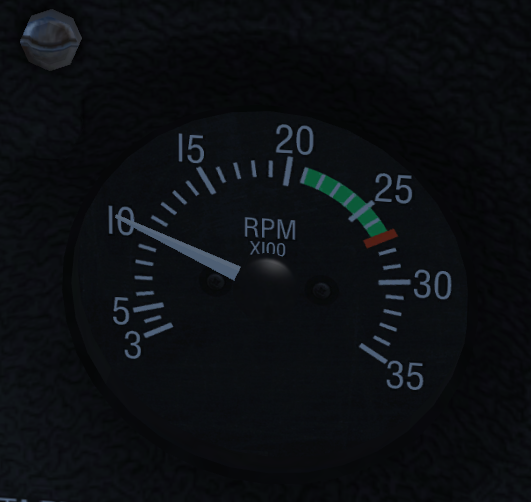
\includegraphics[width=0.35\textwidth]{img/basic_tutorial/tach}
\end{wrapfigure}


默认情况下,启动 \FlightGear{} 会让你正对跑道并准备出发,你也许会想飞机如何从机库,经过滑行道进入跑道的。这就是滑行。

上图是 \Index{转速表}。表示发动机运转时的速度,单位是每分钟百转数(RPM)。

按 \key{PageUp} 键几次,直到转速表显示大概 1000 RPM 左右(如上图)。可以用 \key{PageDown} 降低发动机速度。

在大概 1000 RPM 时,飞机会在跑道上移动,但却不会加速到起飞速度。

\index{刹车!右轮[.](点号)}按 “\key{.}” (Azerty 键盘则是\key{Shift-;})键飞机将会快速向右转弯。如果你一直按着 “\key{.}” 键飞机会刹停。当你按 “\key{.}” 键时会触发飞机右轮刹车。

\index{刹车!左轮[,](逗号)}要触发左轮刹车,可以按 “\key{,}” 键。

\index{刹车}“\key{,}” 和 “\key{.}” 键,模拟了真实飞机上的刹车踏板。使用油门和刹车踏板,你可以控制飞机地面的速度。

在机库和滑行道慢速滑行时左右轮的刹车是非常有用的。你也可以转动飞机前轮。在真实中,飞机前轮是通过用脚蹬踏板实现的。用脚蹬相应方向的脚踏板就会向那个方向转弯\footnote{飞机上的脚踏板又称为“脚蹬”,它同时控制方向舵(包括前轮)和左右轮刹车,不过却用不同的方式。向前方蹬左侧或右侧的脚蹬会控制方向舵偏转,同时带动前轮向左或右转弯。如果向下踩左侧或右侧(当然可以同时踩)的踏板,会触发相应的左轮或右轮刹车。这些操作在 FlightGear 里面都有模拟实现,读者可留心观察“脚下”的动作。——译者注}。如果没有方向舵脚蹬设备,可以用两种方式来虚拟:
\begin{itemize}
    \item 使用小键盘上的 “\key{0}” 键和 \key{Enter} 键\index{方向舵!键盘控制}。如果按小键盘上的 \key{Enter} 键几次,你会看到飞机向右转并一直右转。按 “\key{0}” 键几次,来让飞机恢复直线。
    \item 使用鼠标。当鼠标是驾驶盘控制模式时($+$ 形的鼠标指针),如果你按住鼠标左键并移动鼠标,此时会控制方向舵脚蹬而不是驾驶盘。方向舵脚蹬同时连接着方向舵和前轮。这样控制起来更加精确。
\end{itemize}

启动模拟器,按 \key{v} 或 \key{V} 键从外部来看飞机,按 \key{x} 几次来放大飞机。观察前轮并按小键盘上的 “\key{0}” 键。然后再按 \key{Enter} 键。你可以看到前轮的转动。按 \key{Tab} 键,让鼠标进入控制模式($+$ 形的鼠标指针)。保持鼠标左键按下,进入方向舵控制模式,移动鼠标向左向右。注意此时方向舵,也就是垂直尾翼上的移动面,会与前轮同时移动。

我倾向于在地面上用鼠标控制前轮,在空中用小键盘的 \key{0} 键和 \key{Enter} 键来控制方向舵。也就是说:在地面上我可以用鼠标更加精确的控制前轮来转弯,而当前轮离地以后,我就会放开鼠标左键。

\subsection{空速}
\begin{wrapfigure}{r}{0.35\textwidth}
  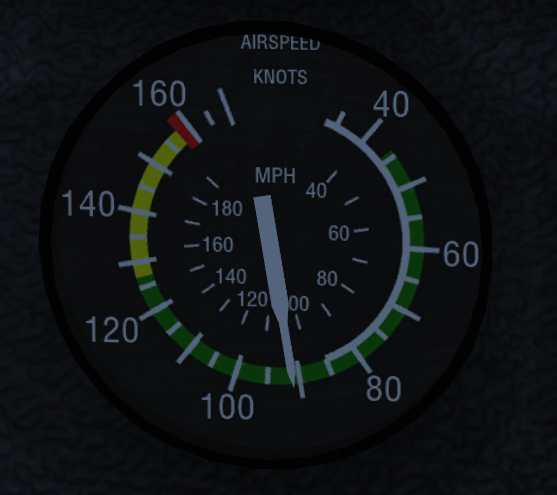
\includegraphics[width=0.35\textwidth]{img/basic_tutorial/airspeed}
\end{wrapfigure}

就像开车一样,知道你运动的速度肯定有帮助。航空上用空速表(ASI)来测量速度,以海里每小时为单位(节)\footnote{1海里是1弧分经线的长度(1852米)。1节等于一小时运动1海里所需要的速度,因此60节就是60海里/小时。}。

\index{速度!单位!节 [海里每小时]}1 节(knots)等于 1.852 千米/小时。因此粗略来说,如果你想换算成千米每小时(km/h)的话,只需将节数乘 2 即可。1 节等于 1.15115 英里/小时(mph),因此非常粗略的,1 节就等于 1 mph。注意很多飞机的空速表(比如 Piper J3 Cub)就是用 mph 而不是节做单位来表示空速\footnote{稍微精确的心算方法:将节数(海里数)乘以 2 再减去 10\%,例如 22 节,先乘以 2 得 44,再减去 10\%,即 44 减 4 得 40 公里,已经很接近精确值 40.31 公里。——译者注,摘自《飞行快速心算》一书,中国民航出版社}。

空速表显示的是飞机与周围空气的相对速度,而不是像汽车速度表那样是相对地面的速度。如果飞机停在地面,而有 10 节的风正对飞机,那么空速表将会显示 10 节的空速,虽然此过程飞机相对地面纹丝未动\footnote{空速表指示的空速一般称为“指示空速”(Indicated Airspeed,IAS),而这一段例子里的“10节”空速其实应为真空速(True Airspeed,TAS),在平均海平面高度且标准大气环境(101.3百帕摄氏15\textdegree{}),指示空速与真空速相等。然而平时为了简便起见,我们还是使用指示空速来操纵飞行。同时飞机相对地面的速度称为“地速”(Ground Speed,GS)。——译者注}。

当飞机在跑道上运动超过 40 节时,你必须避免让前轮接触地面。前轮并没有设计运行在高速状态,在真实状况下前轮会摆动甚至折断。

起飞时,超过 40 节你可以轻柔的拉杆,让前轮离开地面。不要在地面上高速转弯,可能会导致飞机翻覆。

下图展示了前轮轻柔离开地面。不要过度离开地面,保持飞机前盖低于地平线。你只需轻柔抬起前轮。

问题:如果前轮不再接触跑道,如何转弯?回答:依旧使用方向舵踏板。正如前文所述,方向舵踏板同时连接了前轮和尾部方向舵:

\begin{center}
  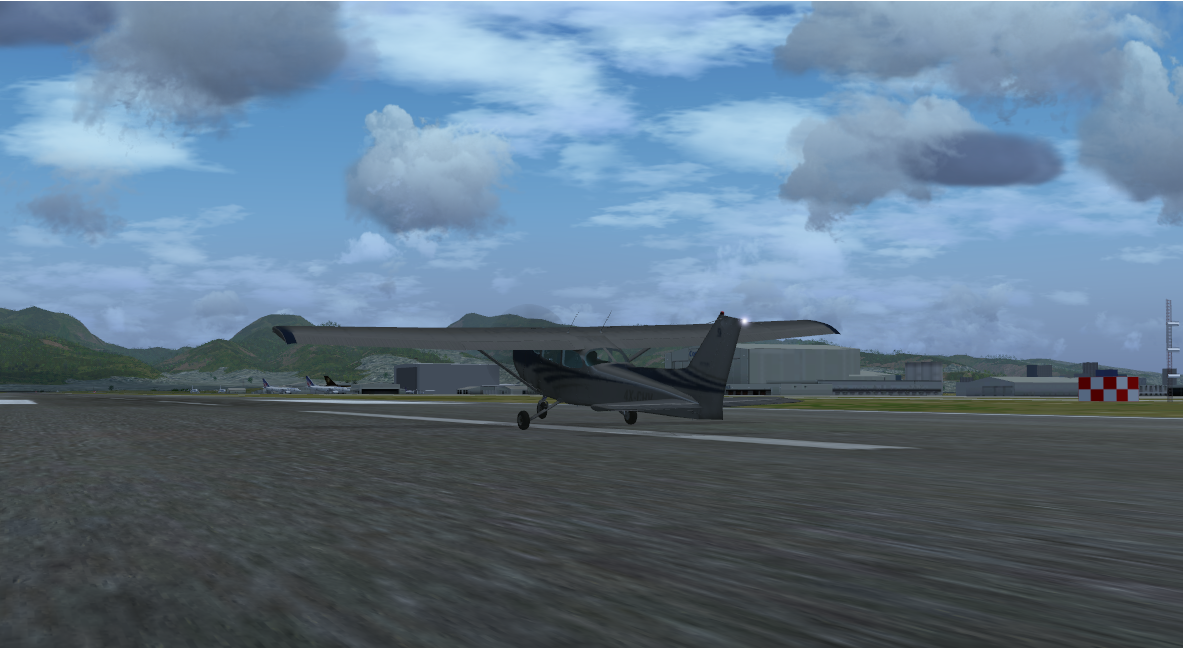
\includegraphics[width=\textwidth]{img/basic_tutorial/rotation}
\end{center}

\begin{wrapfigure}{r}{0.35\textwidth}
  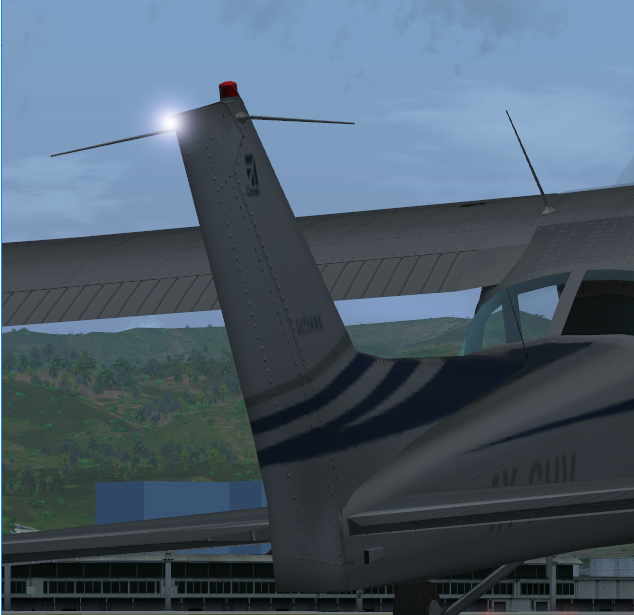
\includegraphics[width=0.35\textwidth]{img/basic_tutorial/rudder}
\end{wrapfigure}

当空速超过 40 节时,方向舵上有足够的空气流过,这样就可以来控制飞机。

注意前轮和方向舵让飞机转弯时的曲率是不同的。所以当用方向舵来控制飞机时,你需要适应方向舵的角度控制。这意味着你需要更快的按小键盘上的 \key{0} 键和 \key{Enter} 键(或者按住鼠标左键用鼠标紧密的控制方向舵)。

当你更加熟悉前轮和方向舵的控制以后,你可以用这些来控制飞机在跑道上直线滑行起飞。

当飞机向右太多时,你按 \key{0} 键数次来纠正。不要等飞机完全对准中心线再转弯,当飞机快要到你想要的方向时,按几次 \key{Enter} 键,否则你会发现要不断面对“过度修正”的问题。如果你用鼠标,修正操作就会变得更容易也更精确。

一言以蔽之,有两种方法控制飞机地面的运动:左右轮的刹车以及方向舵踏板。这种控制冗余在航空业非常普遍。如果一种方法失效,你还有另一种来备份。

你也许会想,为什么飞机在地面会向左倾斜,导致你必须在方向舵上施加向右的力?主要原因是因为发动机扭矩。当螺旋桨顺时针旋转时,就会有一个相反的逆时针旋转的力。施加在左侧主轮和轮胎上。这个力会稍微增加左侧阻力压缩左轮胎半径。第二个原因是流过螺旋桨的空气。这些空气流过机身并因为机身作用形成涡流,涡旋气流的上部会“推”着垂直尾翼向右侧偏,进而导致飞机前部向左侧偏航\footnote{此现象有个专业名词叫“螺旋桨滑流”。螺旋桨飞机左侧偏航又称为“Left Turning Tendency”,除了文中所说的两个原因,还有螺旋桨因子(即 P-Factor)及“陀螺进动”。后两个因素在爬升时影响更大。——译者注}。

你可以用小键盘上的 \key{5} 键将驾驶盘和方向舵置中。飞行前这是个很好的预防措施。有时在飞行中此操作还能“救命”。

\section{高级转弯}
\label{sec:Turning}

就如同在地面一样,空中也有两种转弯方式。你可以如上文所述使用副翼(转动驾驶盘/鼠标)或者使用尾部的方向舵(蹬方向舵踏板/小键盘 \key{0} 键和 \key{Enter} 键)

为什么有两种方式?既互为冗余,又互为补充。方向舵的主要作用是偏航(让飞机绕竖轴旋转),副翼的作用是滚转(让飞机绕纵轴旋转)。

\begin{itemize}
    \item 当飞行离地面很近的时候,最好不要通过滚转来转弯,更多的时候会使用方向舵。方向舵可以让你转弯而飞机不带任何坡度。
    \item 当飞机离跑道很近时,两侧机轮需要保持距离跑道同样高度,这表示机翼必须水平。飞机不允许有坡度。通过副翼来保持飞机机翼水平。注意不需要特别完美,有一点点小坡度是无害的。
    \item 在飞行中,特别是高速时,方向舵转弯是非常低效的:
    \begin{itemize}
    \item 它可以使飞机增加侧翼的气流,进而增加阻力
    \item 飞机转弯很慢
    \item 高速时离心力会非常强甚至有危险
    \end{itemize}
    因此使用副翼可以让你更有效率、快速、可靠且舒适的转弯。
    \item 方向舵在机翼失速时至关重要。因为,在失速时机翼副翼变得低效或者无法使用(注意有些飞机会在低速时,因为过度使用方向舵而进入非常危险的失速)。
 \end{itemize}   

飞行中转弯使用副翼,你依旧需要用一点点方向舵。稍加方向舵可以用来抵消副翼转弯时产生的不利偏航\footnote{这是因为向下偏转的副翼增加了那一侧机翼的升力,而升力的增加也增加了诱导阻力。——译者注}。在真实飞行中,你可以感受到这股侧滑力。在模拟器里你需要关注转弯侧滑仪。下图展示在猛的使用副翼右转时,小球被甩向了右侧。这意味着飞行员也承受着相同向右的侧滑力。你可以通过稍稍向右蹬方向舵来抵消这个力(按 \key{Enter} 键数次)。在正常的飞行中,你需要用方向舵保持小球在中间。

\begin{wrapfigure}{r}{0.35\textwidth}
  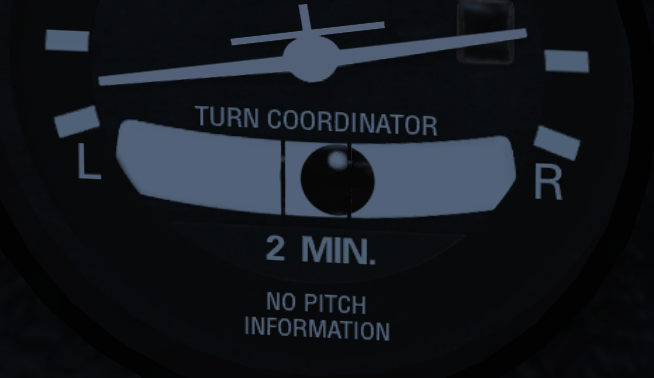
\includegraphics[width=0.35\textwidth]{img/basic_tutorial/turn-coordinator-2}
\end{wrapfigure}

因此在正常飞行中,使用副翼来转弯。当接近地面低速时使用方向舵。一种方式不能完全取代另一种。你依旧需要在高速高空使用方向舵。相反的,你也可以在低空时用副翼来保持机翼水平。

地面滑行时,你也应该用副翼。强风很可能会把飞机吹翻,为了抵消这个,你需要向风的方向转动副翼。向来风的一侧升起副翼,可以帮助机翼向下。

你需要避免快速而粗暴的移动方向舵。在地面,这会造成飞机快速旋转。在空中低速时会造成非常危险的一种失速,高速时会造成空气动力学部件和物理损坏。所以对待方向舵要温柔。

我建议你在飞行时练习使用方向舵。在低速,比如 70 节时,通过增加和减少发动机功率来保持高度。用方向舵转向一个地面景物并保持航向,然后再将飞机转向新的航向。观察飞机如何偏航,并学习预判方向舵的控制。不要尝试陡峭的转弯,使用副翼来保持机翼水平。

\section{这些是什么?}

这一章将会讲解飞机的仪表、开关和飞机的控制。虽然在模拟飞行里,你只需要通过油门和驾驶盘就可以控制飞机的基本操作,然而你需要了解所有控制方式以便更安全和高效。

\subsection{发动机控制}
\label{sec:EngineControl}

飞机的发动机被设计成简单、可靠和高效的。与现代汽车使用高级电力点火和燃油喷射系统不同,飞机使用老式技术而不依赖电能。因此当飞机电力完全失效的时候,飞机依旧可以飞行。

\subsection*{磁电机}\index{磁电机}

在仪表板左下角你可以找到磁电机的的开关和发动机点火开关:
\begin{wrapfigure}{r}{0.35\textwidth}
  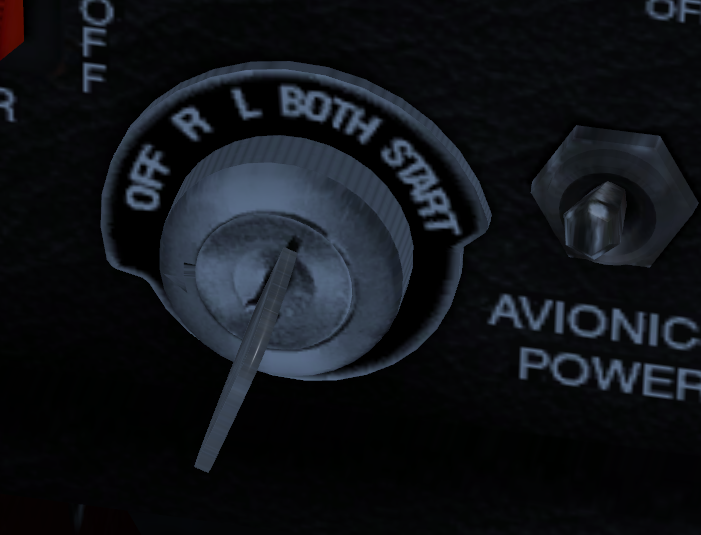
\includegraphics[width=0.35\textwidth]{img/basic_tutorial/mags}
\end{wrapfigure}

要看清此开关,可以按 \key{P} 键查看 2D 概要仪表板,或者按 \key{Shift-x} 来缩小(用 \key{x} 键或者 \key{Ctrl-x} 恢复缩放)。

也许你知道汽车使用电动火花塞来引燃汽油。现代汽车引擎使用电力点火装置。飞机发动机则使用更加老式(但更可靠)的磁电机点火开关。为了冗余设计,包括左和右两套磁电机。当你将磁电机转换到 OFF 位时,两侧的磁电机都会关断,发动机也会停止。将磁电机开关转到 L 位则会使用左侧的磁电机,转到 R 位则使用右侧磁电机,在 BOTH (双侧)位则同时使用两侧的磁电机。在飞行中我们使用 BOTH 位。

既然在飞行中我们使用双侧磁电机,为何还要有切换开关?原因是在飞行前我们需要检查所有磁电机都工作正常。要检查磁电机可以将发动机转速设置在 1500 RPM 并切换磁电机到 L 并观察转速表。你能观察到转速有小幅下降。如果发动机被切断,左侧磁电机故障。如果你没有看到转速下降说明切换开关有问题,因为双侧磁电机都在工作。你可以用同样的方式来检查右侧磁电机。当然在模拟飞行里,磁电机是不会故障的!

在飞行中如果一个磁电机故障,那么另一个会保持发动机运转。单侧磁电机失效是很罕见的,双侧都失效几乎没有听说过。

你可以按 \key{\{} 键来关闭发动机。要起动发动机可以按 \key{\}} 键三次以便让磁电机切换到 BOTH。然后按 \key{s} 键使用起动机,按住几秒钟,直到发动机起动。

你可以通过正常模式的鼠标转动磁电机开关。按 \key{Ctrl-c} 来查看以黄色矩形框高亮出来的可操作区域。

如果你将磁电机开关置为 OFF 位,发动机噪音就会停止。此时如果快速切换到 L 位,发动机又会起动螺旋桨依旧旋转。如果你一直等到螺旋桨停止,再切换到 L、R 甚至是 BOTH 位,都不会起动发动机。当发动机停止时,永远要将磁电机开关置为 OFF 位。

\subsection*{油门}\index{油门杆}

\begin{wrapfigure}{r}{0.35\textwidth}
  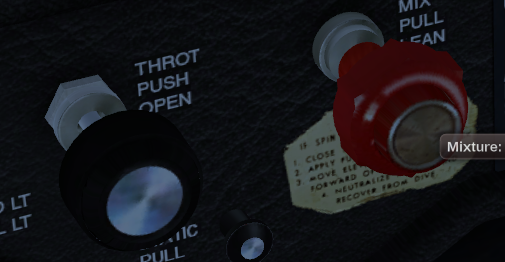
\includegraphics[width=0.35\textwidth]{img/basic_tutorial/throt-mix}
\end{wrapfigure}

你已经知道通过推油门杆(按 \key{PageUp} 键)可以增大发动机动力,拉出油门杆(按 \key{PageDown} 键)可以减少发动机动力。在油门杆上按鼠标左键和右键也有相同的效果(鼠标中键可以快速移动。按 \key{Ctrl-c} 来查看以黄色矩形框高亮出来的可操作区域)。

“增大动力”到底是什么意思?是不是意味着将输入发动机的油量增加?是的,但这并不能完全解释。你需要知道飞机发动机也需要大量空气。发动机的汽缸里燃烧的是\Index{油气混合}物质。只有燃油是不能燃烧的。必须是一定比例混合的燃油和气体,才能爆开和移动发动机的活塞。所以当你推油门杆的时候,同时增加了燃油和空气到发动机里。

\subsection*{油气混合}\index{油气混和}

一定的空气遇上一定的燃油是非常危险的。必须时刻密切关注这两者的比例。这也正是油气混合杆的作用。下图展示了油气混合比杆,已经拉出很多。

当\index{油气混和\混合比杆}混合比杆完全推进的时候,进入发动机的是大量燃油和少量空气。这就是所谓的“富油”混合。当油气混合比杆被完全拉出的时候,将会有过量的空气进入发动机,也就是“贫油”混合。正确的混合比则是在这两种极端之间,多数情况会比较接近完全推入状态\footnote{一般最佳的油气混合比是 15:1,即15份空气需要1份燃油。——译者注}。

当你起动发动机和起飞的时候,你需要富油混合。这意味着混合比杆需要完全推入。富油混合可以让发动机更容易起动,也会让发动机多了一些可靠性。缺点是一些油并不会完全燃烧,只会造成浪费并被排出。这会让发动机变得很脏,同时降低了发动机的输出功率,并因为残积物堵住汽缸而慢慢劣化发动机。\index{油气混和!优化}

在正常飞行中,你需要将油气混合杆稍向后拉,以获得最佳油气混合比。在模拟器里可以这么做。启动模拟器以后,设置停留刹车,按 B 键(\key{Shift-b})。将油门推到最大,发动机转速此时会接近最大转速。慢慢拉油气混合比杆(使用正常模式下的鼠标)。你会看到转速有小幅升,你获得了更多的动力,而没有增加燃油量。你没有浪费燃油也减少了污染。如果你继续拉油气混合比杆,转速又会开始下降,因为现在空气太多了。过量的空气减慢汽缸里的膨胀速度,并降低了膨胀温度,因此热度下降。你必须优化混合比。因为热力学的原因,最佳混合比不会恰好产生最大动力——至少好过发动机只比最大动力轻微富油或者贫油。这样也能避免燃油的爆燃损坏发动机。你可以通过检查最高转速来获知最大动力。另一种方式是检查发动机的排气管温度。粗略来看,当温度最高时动力最大。

控制混合比还能让你在同样速度和距离上,燃烧更少的燃油,这样可以飞的更远并减少污染。然而若你不懂如何控制它,将会产生很严重的问题。假设你在高空将油气混合比杆拉出,高空氧气含量较少,因此高空正确的混合比需要更贫油,也就是更少的燃油使用。然后你准备降落开始下降。如果下降时你忘记将油气混合比杆推多一些,导致油气混合变得越来越贫油,直到发动机停止。

降落时,你需要将油气混合比调到稍微富油,也就是将混合比杆推多一些。这会让发动机更可靠一些并可以更好的适应高度的下降。

我在上文讲磁电机的时候,将磁电机置 OFF 位并不是让发动机关车的好方法。正确的做法是将油气混合比杆拉出\index{发动机!关车}。首先将油门杆完全拉出,这样可以让发动机耗油最少。然后拉出油气混合比杆,直到发动机因为混合了太多空气而停止。这可以确保发动机不会因为废燃油堵住。最后将磁电机置 OFF 位确保发动机不会突然起动。

一个很重要的警告:你也许会以为转速表反映了发动机的动力。错。两个因素会让动力增加:发动机输出功率和飞机的速度。为了验证这个,飞到某个高度然后将发动机减到最低。尝试向地面俯冲,然后回到刚才的高度。你会看到转速表在你速度变化时有显著变化。它会在俯冲时变大在爬升时变小。

这带来的一个陷阱是当你打算降落时。假设你正在快速下降进入机场。你知道理想的降落转速大概是 1900 RPM。因此你将油门拉出,得到 1900 RPM 的转速。你认为使用了合适的转速,不再需要为此烦恼。然而当你拉平,飞机的速度开始降低,因为转速低。几分钟后飞机速度达到你预期的低速。你没再注意转速已经很慢了。此时你要么会掉高度,要么就会失速,也许两者都会发生。因此请注意油门和转速表。注意收油门的时候要更稳定,要随时准备将油门快速推回。

\subsection{机翼和速度}
\label{sec:WingsAndForce}

假设你正在全动力飞行。轻微降低机头会让你降低高度而抬升机头则可以让你升高。你也许会想这很简单嘛。飞机飞行时的航向就是螺旋桨的指向。而这并不是最好的思考方式。此模型也许适合描述火箭,但不适合一架飞机。火箭是靠其引擎推进,而飞机则是靠机翼。这有巨大的差异。

找一个正方形的硬纸板,水平放在你的手上,手臂伸开并在水平方向快速移动。当纸板平着穿过空气是不会产生升力的。如果你将手臂旋转,让纸板有一个向上的角度,你会感觉到纸板将要飞到空中,一个向上的力作用在纸板上。这就是机翼让飞机留在空中的原理。给纸板越多角度,其升力就越大。直到角度越来越陡峭,你会感觉到下降。纸板进入“失速”状态(请接着看下文)。

\centerline{
  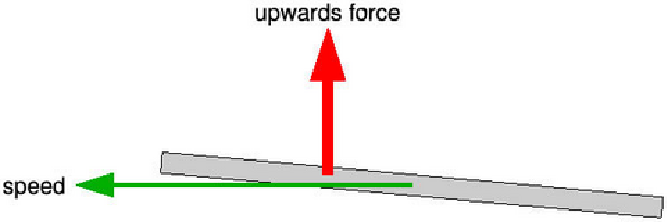
\includegraphics[width=0.5\textwidth]{img/basic_tutorial/lift}
}

\begin{itemize}
    \item 当你拉驾驶盘的时候,飞机机头向上。机翼以一个陡的角度穿过空气,因此机翼上的升力就变强了,飞机就升入天空。
    \item 当你推驾驶盘的时候,飞机机头向下,机翼与气流的角度变小,机翼上升力变弱,导致飞机下降。
\end{itemize}

重要的是机翼穿过空气时的角度,这就是迎角(Angle of Attack,AOA)\footnote{注意迎角是飞机翼弦线与相对气流之间的锐角,为了更好的理解这个概念,下文有精彩的讲解。“迎角”的另一个中文翻译是“攻角”,但不太常用。——译者注}。

上面说如果机翼穿过空气的时候没有角度,将不会产生升力,这是错的。如果机翼像硬纸板那样全平的确实如此。但是机翼都有一个稍微弯曲的翼型。这就让机翼可以在没有迎角时,也能产生升力。甚至上在反向角度时,也能产生升力。高速飞行时飞机是会稍微指向地面的!

\centerline{
  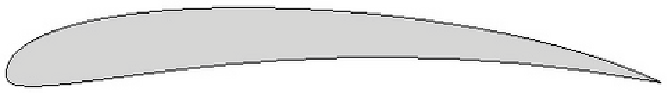
\includegraphics[width=0.5\textwidth]{img/basic_tutorial/airfoil}
}

机翼穿过空气是一方面,另一方面则是速度。还是用硬纸板举例,现在不改变纸板的角度,用不同的速度移动手臂,你会发现移动速度越快,则其升力越大。

\begin{itemize}
    \item 增加发动机动力,飞机速度加快,增加机翼升力,飞机会上升高度。
    \item 降低发动机动力,飞机速度减慢,减小机翼升力,飞机会降低高度。
\end{itemize}

稍微复杂一些:为了升的更高,飞机会倾向于丢失速度。而为了降低,则得到了速度。

这些都需要折中考虑。如果你想在恒定的高度以给定速度飞行,你需要同时调整发动机动力和驾驶盘/副翼(或者最好使用调整片,下文详述),直到获得你所需的高度和速度。如果你想以同样的速度下降,你需要轻轻推杆并收油门。也就是说你经常需要同时调节发动机动力和驾驶盘。不过,在正常飞行中,可以先调整发动机动力到合适的位置,然后再通过驾驶盘或调整片控制高度。

模拟器里你可以做这样的有趣实验,全速直飞,在水平飞行时尽可能获得最大速度。然后将发动机调到最低动力(慢车),然后控制飞机驾驶盘使飞机保持高度。飞机会慢慢下降,同时你需要更加努力向后拉杆以保持飞机水平。因为速度降低,机翼上的升力也降低,但是你通过增加迎角的方式补偿了速度的损失。这证明了飞机不是按照其机头指向航行。在此实验中,我们让机头抬起来保持高度,当飞机越来越慢,机头也会抬的越来越高,此时你会听到一声尖锐的警报,这就是失速警报(下文详述)。这表示飞机的迎角太大,以至于机翼翼型无法产生足够的升力,机翼不能产生升力,飞机会迅速下降。唯一解决办法是推杆来减小迎角,让机头下降并推发动机动力到最大来获取速度。最后慢慢恢复正常驾驶。

问题:控制飞机的高度和速度,用油门还是用驾驶盘,哪个更好?回答:这取决于你具体的情况。在正常飞行中,你会倾向于先设定合适的发动机动力,然后依靠驾驶盘和调整片。在起飞和降落阶段,使用驾驶盘和油门的程序比较复杂和严苛,与之前相反,先用驾驶盘和调整片控制速度,进而用油门控制高度并降低速度。下面的章节会深入讨论。

\subsection{襟翼} \index{襟翼}
\label{sec:Flaps}

襟翼是机翼后缘靠近机身两侧的活动部件。你可以使用襟翼控制杆来放出和收起机翼\index{襟翼!控制杆}:

\centerline{
  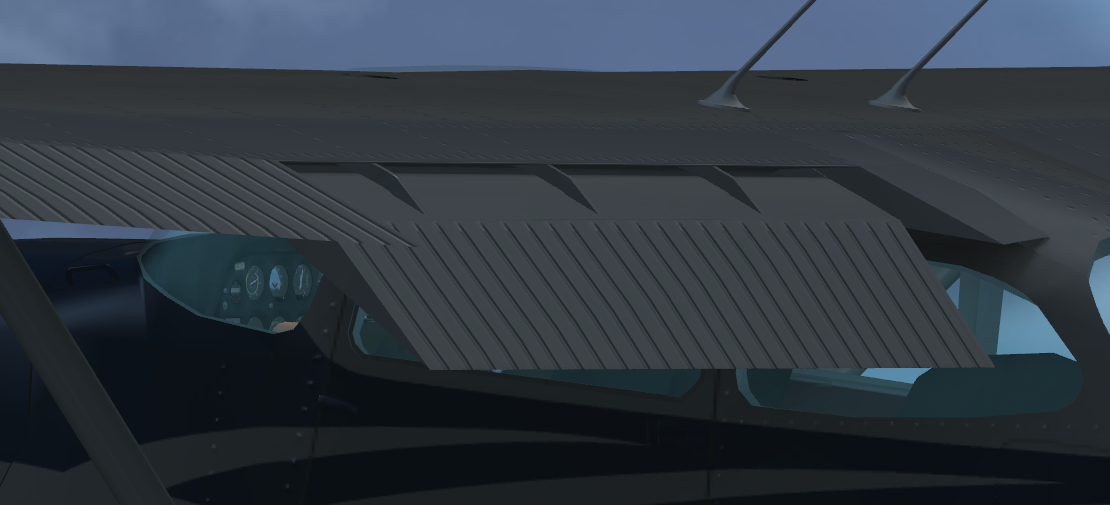
\includegraphics[width=0.6\textwidth]{img/basic_tutorial/flaps}
  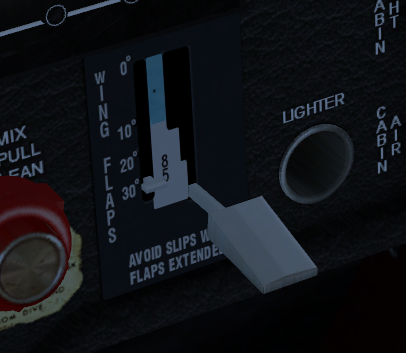
\includegraphics[width=0.315\textwidth]{img/basic_tutorial/flaps-ctl}
}

你可以用鼠标点击,也可以使用 \key{[} 和 \key{]} 键来控制。 \key{[} 键会收一档襟翼,\key{]} 会放出一档襟翼。按  \key{v} 键从外面观察并尝试用 \key{[} 和 \key{]} 键收放襟翼。

塞斯纳 172P 有四种襟翼设定\index{襟翼!阶段}:
\begin{itemize}
    \item 0\textdegree{}:正常飞行和起飞时使用。
    \item 10\textdegree{}:用于短跑道起飞,慢速飞行时获取高度,或者进近着陆的第一阶段。
    \item 20\textdegree{}:用于快速降低高度和速度,比如对正跑道准备落地时 
    \item 30\textdegree{}:用于更快的降低高度。
\end{itemize}

襟翼是很脆弱的,不要在速度 110 节以上时放出襟翼,也不要在 85 节以上速度时放出第二和第三阶段襟翼。

襟翼可以制造大量的阻力,这就是为什么在高于 85 节或 110 节时收起襟翼。

要检查襟翼的位置,可以使用鼠标的查看模式,回头看襟翼。也可以用 \key{Shift}-\key{右箭头} 快速切换到右侧查看,并快速使用 \key{Shift}-\key{上箭头} 回到原来的向前视角。

襟翼通过改变翼型以获取升力,放出第一阶段襟翼时在同等速度下机翼获得了更大的升力。这样你可以在起飞后更快飞入天空,同时也可以影响机头高度,这样可以在起飞和降落阶段有更好的视野。

襟翼也增加了飞机的阻力。第二和第三阶段襟翼产生的阻力大于升力,因此用襟翼可以让飞机减速。这在降落时非常有用,因为飞机滑翔性能非常好,如果你关闭发动机,飞机将会下降虽然很慢。你需要放出两档或三档襟翼来减速并向地面下降。

实际上襟翼在降落阶段需要更大的发动机动力。这会有些奇怪,为什么不将油门杆拉到最低并使用更少的襟翼呢?这是为了获得更好的减速效果和更多发动机动力,这样飞机可以更快的响应你给出的指令。当发动机失效时,收起襟翼并滑翔到跑道即可。

\index{侧滑}
如果襟翼全部放出,而你需要更多的下降怎么办?慢慢蹬方向舵到某个方向,这将会让飞机侧翼承受气流并减速。然后通过适当转动驾驶盘(操作副翼)来补偿滚转倾向。这就是所谓的侧滑(Side-slip),这是一种有效降低高度的手段并可以在任何阶段改出\footnote{使用侧滑法仅可用来降低高度,飞行中任何时候使用这种交叉控制都会带来很大风险,容易失速并很快进入螺旋,特别是低空转弯时,协调控制副翼和方向舵进行转弯。使用侧滑法降低高度最有名的例子,是 1983 年加拿大航空 143 号客机(机型 767-233)因为燃油耗尽导致发动机空中停车。飞行员使用侧滑方式快速降低高度和速度,在最近的赛车道迫降成功。相关详情:\web{https://en.wikipedia.org/wiki/Gimli\_Glider}。——译者注}。

\subsection{失速}\index{失速}
\label{sec:Stall}

飞机依赖机翼上流过的平滑气流来产生升力。然而若机翼的迎角太大,则会造成气流破碎,这样就不会产生升力。没有升力飞机就不能飞行,很快就会落回地面,这就是失速。

失速是一种危险的状况,任何速度下都可能会发生,通常慢速飞行时更容易发生。飞行器都有一个失速速度,低于这个速度任何迎角都不能产生升力。你需要始终让飞机保持在失速速度以上。为此,飞机都安有警报器,在接近失速迎角时,会发出声音警告。

如果你进入了失速,补救措施是尽快降低机头,并增加发动机动力到最大,随后当速度恢复后将机头拉平。然而这么做会让飞机失去高度,因此在降落和起飞的时候,绝对不能进入失速状态!

\index{螺旋}当一侧机翼比另一侧先失速时,一般会在低速大坡度转弯时发生,此时飞机会进入螺旋。因为一侧机翼还在提供升力,飞机会围绕失速一侧的机翼旋转,越转越快\footnote{此处作者讲述有误,螺旋发生时两侧机翼都处于失速状态,只是一侧的失速程度更深。——译者注}。为了从螺旋状态改出,你需要先用方向舵让飞机停止偏航运动,进入普通的失速,然后再如前文那样改出失速\footnote{通常来说,从螺旋中改出的动作第一步是油门慢车、副翼中立,在确定旋转方向后,使用最大行程的反舵,制止旋转。对于某些飞机仅需松杆就可以从失速中改出,但有的飞机则需向前推杆以改出失速。当旋转减慢,逐渐回平方向舵,以避免进入反方向螺旋。当螺旋停止且方向舵回平时,逐步带杆退出下降。过多或突然的带杆或在恢复过程中使用副翼或未及时回平方向舵可能会导致二次失速和另外的螺旋。——译者注,摘自中国民用航空局飞行标准司-咨询通告,编号AC-61-FS-2013-19}。

像塞斯纳 172P 和 Piper Cub 这样的飞机,会很容易进入失速,但却很少能进入螺旋。而高速喷气式飞机,比如 F16 则很容易进入螺旋,却不太容易达到失速。

要在模拟器里练习失速,可以如此:
\begin{itemize}
    \item 飞到一个恒定的高度和姿态。
    \item 降低发动机动力,并抬升机头避免下降。
    \item 继续减少发动机动力直到进入失速
    \item 尝试控制住飞机避免向地面下落
    \item 保持驾驶盘拉到最大位置,稳定飞机的姿态,机翼与地平线平行。尝试改变方向。
    \item 通过降低机头,推油门到最大来改出失速,当速度恢复以后修正姿态\footnote{安全起见,整个失速改出练习高度不应低于 1500ft AGL。——译者注}。
\end{itemize}

你可以用不同的襟翼配置练习失速改出,或在高速飞行时突然改变姿态进入失速。

还可以尝试使用不同的机型,比较一下塞斯纳 172P 和塞斯纳“奖状”(Cessna Citation)喷气式飞机在失速表现上的异同,会发现失速更突然,而只有很少的警报。
\newpage
\subsection{升降舵调整片}\index{调整片}
\label{sec:Trim}
\begin{wrapfigure}{r}{0.35\textwidth}
  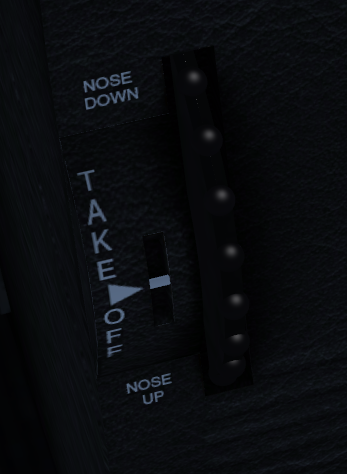
\includegraphics[width=0.35\textwidth]{img/basic_tutorial/trim}
\end{wrapfigure}

升降舵调整片拨轮是一个黑色竖直的轮子,中间有灰色的点状突起。在仪表板下方可以找到:

在 \FlightGear{} 中,使用 \key{Home} 键和 \key{End} 键控制调整片。\key{Home} 控制拨轮向上转, \key{End} 控制拨轮向下转。你可以在拨轮上方和下方点击来控制。

近似来说,调整片与驾驶盘的作用是相似的,也可以完成升降舵的操作。向下转动拨轮,相当于向后拉驾驶盘。然而有个巨大的不同,那就是调整片调整以后会保持位置,而驾驶盘除非你一直施力影响,放开驾驶盘会自动回中。

巡航阶段,为了维持飞机在恒定的高度,副翼可能不在中立位——依赖飞机周围的空气,当前的燃油量和配载。显然,飞行员一直控制着驾驶盘维持高度很快会疲劳。使用调整片可以“卸掉”升降舵上的力,驾驶盘也可以回中。

在起飞阶段,调整片必须回中。否则你会发现要么飞机抵抗起飞,很难拉起机头到正常位置,要么很快就起飞了。

在降落阶段,善用调整片让你的升降舵在中立位。这样只需小幅调整姿态就可以很容易控制了。对塞斯纳 172P 来说是调整片回中,而对 Cherokee Warrior II 来说就是调整片“拉出”。

调整片拨轮的移动比驾驶盘慢的多,允许精细的调整片操作。操作时请耐心一点。

\subsection{我的飞行方位是?}
\label{sec:Kierunek}

知道你的飞行方位显然是个好主意。有三种方式来获取你在空中的位置:
\begin{itemize}
    \item 透过窗外景物。识别地面特征,比如道路、山丘、桥梁、城市、森林等。在模拟器中,你只能使用很狭窄的观察窗口查看虚拟世界。有如下方式让你可以在飞机里平移视角。
    \begin{itemize}
        \item 使用 \key{Shift} 键搭配四个方向键来观察前后左右。
        \item 使用 \key{Shift} 和小键盘的按键来观察前后左右,还有斜前方斜后方。
        \item 在正常模式或控制模式按住鼠标右键,同时移动鼠标观察四周。
        \item 在鼠标的查看模式(使用 \key{Tab} 键切换鼠标指针是 $\leftrightarrow$ 时)。这可以让你查看任何位置,包括上和下。按鼠标左键,可以回复正中。
\end{itemize}
\item 磁罗盘。位于仪表板正上方,罗盘非常简单,但却能很好的帮助飞机飞行。另外磁罗盘在地面会受到干扰而异常,还有磁罗盘指向的是磁北极,而不是地理北极,相应的差异与你所在的地区有关系\footnote{有关地区磁偏角相关内容可参考:\url{https://en.wikipedia.org/wiki/Magnetic_declination}。——译者注}。

\item 方位陀螺仪(如下图)或称“航向指示器”(Heading Indicator)。陀螺仪由一套真空系统驱动,与磁罗盘匹配,但不会受到磁力和飞机移动的影响。然而因为陀螺进动和摩擦的影响,一段时间以后陀螺仪会漂移,需要参考磁罗盘重置陀螺仪。要重置方位指示器,在巡航状态下,使用仪表左下角的黑色旋钮。在鼠标正常模式下,用鼠标点击旋钮左半边或右半边来调节,按鼠标中键可以更快调节。可以用 \key{Ctrl}-\key{c} 查看可操作的高亮区域。右下角的红色旋钮是用来告诉自动驾驶仪你打算飞的航向(\textcolor{red}{\button{HDG}} = “航向”(Heading)。

\centerline{
  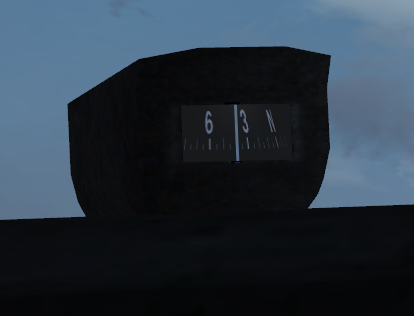
\includegraphics[height=6.0cm]{img/basic_tutorial/compass}
  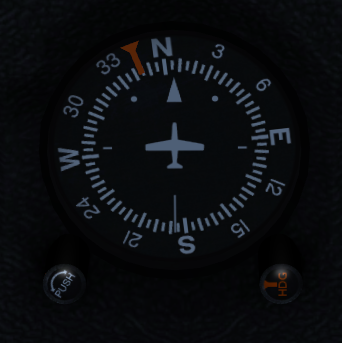
\includegraphics[height=6.0cm]{img/basic_tutorial/DG}
}

\subsection{关于仪表板}

最后让我们来看看仪表板,上面介绍了一些,下面介绍剩下的:

\subsubsection{六块主仪表}

\begin{wrapfigure}{r}{0.35\textwidth}
  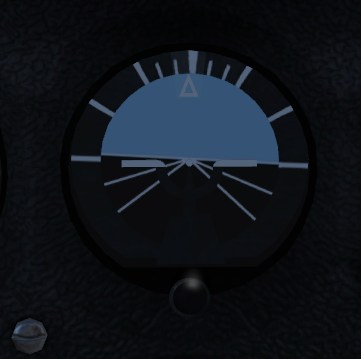
\includegraphics[width=0.35\textwidth]{img/basic_tutorial/attitude-indicator}
\end{wrapfigure}

让我们从最重要的仪表开始,任何模拟飞行员都必须了解的,被称为“holy six”或者“six-pack”的主仪表。

仪表板正中靠上(见图 5)的是\Index{人工地平仪}(\Index{姿态指示器}),显示了飞机的\Index{俯仰}和\Index{横滚}角度。俯仰和横滚都都标示了 10、20、30、60 和 90 度这几个刻度。

人工地平仪的左侧,你可以看到\Index{空速表}。除了指示空速以外,空速表还标出了一些你必须关注的\Index{速度指标}。首先绿色弧线表示\Index{襟翼}全收时空速可操作范围。白色弧线表示使用襟翼时的范围\footnote{白色弧线应表示的是放出全部襟翼时可用的空速范围。——译者注}。黄色弧线表示只可在平缓空气中使用的警戒速度范围。其他的红色表示绝对不可超过的界线,除非你想让飞机在空中解体……

在空速表下方你可以找到\Index{转弯协调仪}。中间的小飞机指示了你飞机的横滚。如果小飞机的左机翼或右机翼处在标线的位置,说明是一个标准转弯,也就是转 360 度需要精确的两分钟。

在小飞机下方,还是在转弯协调仪里,是\Index{倾角仪}。它用来显示\Index{方向舵}和\Index{副翼}是否配合良好。在转弯时,你需要始终协调操作\Index{副翼}和\Index{方向舵}并保持管子里的小球处在正中的位置。否则飞机会侧滑。一个简单的规则是“跟着球走”,比如当球向左手边移动时,就向左侧蹬方向舵。
\medskip

如果你没有方向舵踏板,或者对方向舵和副翼之间的操作比例,没有经验的话,你可以在启动 \FlightGear{} 时使用 \texttt{-$ $-enable-auto-coordination} 选项。\index{自动协调}

在人工地平仪的右侧,你会看到\Index{高度表},显示了飞机距离海平面(不是地面!)的高度,用百英尺表示。在高度表下方是\Index{升降速率表},指示了飞机爬升和下降时的速率,单位是百英尺每分钟。你会发现在某些情况下,升降速率表比高度表更舒服,注意升降速率表会有一定时间的滞后。

在升降速率表下方的是螺旋桨转速表,或者 RPM(Rotations Per Minute)指示器\index{转速指示器}。以每分钟百转为单位。绿色弧线表示巡航时的最佳范围。

主仪表板还包括\Index{陀螺仪罗盘},就在人工地平仪的下方。除此之外还有仪表板中间最上方的\Index{磁罗盘}。

你会发现四块最重要的仪表构成了“T”字形:空速表,人工地平仪,高度表和罗盘。你需要在飞行时不断扫描这些仪表\footnote{扫描仪表的一个方法是,目光叮住人工地平仪,同时快速横向扫描空速和高度,恢复叮住地平仪,再向下扫描罗盘。多多练习在不同飞行动作时扫描仪表的方法,最终熟能生巧。——译者注}。

\subsubsection{辅助仪表}

除了这六块主要仪表,还有很多辅助仪表。最左侧你能看到\Index{时钟},对于计算转弯至关重要。时钟下方有很多小标尺,表示发动机的各种技术参数。其中最重要的是\Index{油量表}——飞行员必须知道。

\Index{点火开关}在仪表板的左下角(见图 4)。有四个位置“OFF”、“L”、“R”和“BOTH”。第一个很显然,“L”和“R”不代表左右两台发动机(塞斯纳 172P 只有一台)而是代表两个磁电机,用来在故障时提供冗余。两个开关位用来在飞行前测试。在正常飞行中开关需要置为“BOTH”。磁电机开关的最右一档是用来\Index{起动发动机}的,使用一个电力驱动的\Index{点火器}(使用 \key{s} 键操作)。

在驾驶盘下方的是驻留刹车。竖直时表示设置了驻留刹车(ON),否则表示驻留刹车解除(OFF)。使用 \key{B} 键控制。

\subsubsection{无线电}

仪表板右手边的是\Index{无线电栈}。你可以看到两台 \Index{VOR} 接收机(NAV)\index{NAV},一台 \Index{NDB} 接收机(\Index{ADF})和两台\Index{无线电通话}电台(COM1/2)\index{COMM1}\index{COMM2}以及自动驾驶仪。

\Index{无线电通话}电台用来和\Index{空中交通设施}通话;它只是使用特殊频率范围的普通无线电收发装置。其频率用 LED 显示出来。一般有两台 \Index{COM 收发机};这样你可以收听下一个要联系的管制员的同时,依旧保持与前一个的联系。

COM 无线电可以用来收听机场当前的天气状况,也就是 ATIS。要这么做只需要调到相应机场的 ATIS 频率即可。你可以从 \texttt{ATC/AI->Frequencies} 菜单项找到邻近机场的 ICAO 四字代码。

每台 COM 无线电有两个频率配置,一个“活动”的频率也就是此时飞行员正在联系的,另一个“备用”的频率是用来改变的。这样你可以守听一个频率的同时,调节另一个频率。

可以用鼠标改变无线电频率,用鼠标点击相应旋钮的左右两侧,通信旋钮旁边的开关用来切换活动频率和备用频率。

后面的章节将会讲到使用自动驾驶仪和无线电导航设备。此刻你可以忽略无线电仪表,因为你现在遵循的是\Index{Visual
Flight Rules 目视飞行规则}(\Index{VFR})。

\section{让我们去飞吧}

到现在为止,你已经会平直的飞行了,也学会了起飞时使用方向舵来维持角度,还学会了下降、爬升和温柔的转弯。这一节我们将会教授更加真实的起飞和降落,还有一些你需要知道的深入理念。

\subsection{真实的起飞}
\label{sec:Start}

下面的原则是正常起飞时需要关注的:

\begin{itemize}
    \item 前轮需要在 40 节时离开跑道。
    \item 起飞后你需要立刻加速到 70 节,高于失速速度,以应对突然的阵风或者发动机失效。
    \item 不要超过 75 节,这样可以让你尽快获得想要的高度。
    \item 爬升到 500 英尺之前要一直沿着跑道方向,以防此时发动机失效,这样你可以直接落在跑道上。
    \item 飞越建筑物至少要 1000 英尺。
    \item 离地比较近时要温柔的转弯,并适当使用方向舵。
\end{itemize}

所以,你需要稳定在 75 节来起飞和爬升。然后在 40 节轻抬机头,飞机会在大概 55 节就起飞了。为了尽快加速到 75 节,你需要在起飞后慢慢降低机头,然后到达 75 节,你再通过驾驶盘来控制速度。

把以上所有之前学到的放到一起,使用鼠标来完成一次正常起飞如下:

\begin{enumerate}
  \item 首先调整高度表到正确的高度,主要是机场标高。比如 PHNL 是在海平面高度 —— 0 英尺。
 \item 观察副翼和升降舵都已经回中,可以观察驾驶盘来确定\footnote{此时最好按小键盘上的 \key{5} 键确认回中。——译者注}。
 \item 按 \key{Tab} 键让鼠标进入控制模式。
 \item 按住鼠标左键来控制方向舵。
 \item 发动机动力推到最大(按住 \key{PgUp} 键,直到油门杆完全推入)。
 \item 当飞机在跑道上加速时,用鼠标做一些细微调整以使其保持中间。
 \item 在 40 节时,松开鼠标左键,轻轻抬起前轮。现在鼠标在控制驾驶盘。
 \item 飞机将会在大概 55 节时飞离跑道。
 \item 慢慢降低机头加速到 70 节。
 \item 保持与跑道中线对齐
 \item 用驾驶盘稳定速度在 70 节爬升。如果空速降低,则推驾驶盘,否则拉驾驶盘。
 \item 到 500 英尺高度,向你需要的航向转弯,飞越建筑物至少需要 1000 英尺。
\end{enumerate}

\subsection{降落}\index{landing}
\label{sec:Ladowanie}

降落几乎和起飞一模一样,只不过顺序相反:

\begin{itemize}
    \item 邻近地面,转弯要温柔并恰当配合使用方向舵。
    \item 最后进近落地之前,保持 500 英尺以上。
    \item 进入跑道时在 70 节左右。
    \item 55 节时两侧机轮接地
    \item 40 节时让前轮接地
\end{itemize}

如果你能在跑道上找出一个瞄准点,对着这个瞄准点落地,那么就会简单许多。观察这个瞄准点,你可以很容易的了解,降落的是否太快或者太慢。如果瞄准点向上移动了,说明你下降的太快。

显然你需要对准跑道。这就意味着你的飞行方向与跑道中线一致(如下图中的 a)。为了可以对准跑道,不要瞄准跑道的起始位置(如下图中的 b),而是瞄准跑道前方一个虚构的点(如下图中的 c),然后离这个虚构点还有一段距离时开始温柔的转弯对准跑道(如下图中的 d)。注意在降落转弯过程中,你的操作必须非常轻柔。你甚至没办法注意转弯协调仪,这就是为什么要依赖外部地平线,而不是飞机仪表。

\centerline{
  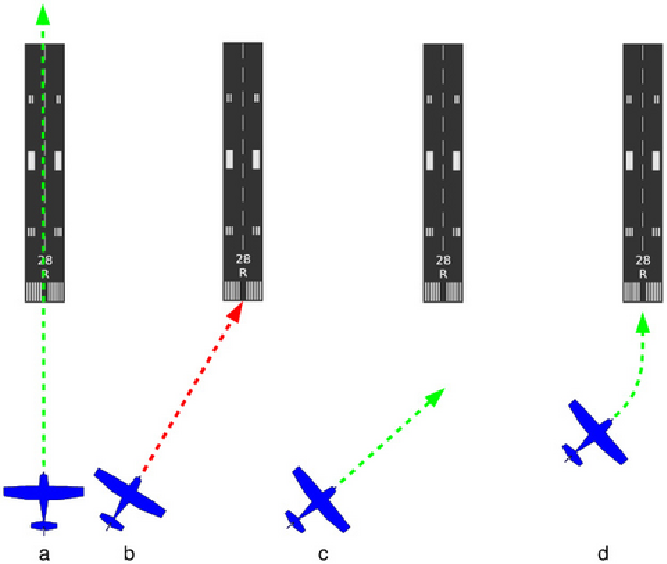
\includegraphics[width=0.65\textwidth]{img/basic_tutorial/runway-alignment}
}


使用鼠标降落的基本流程如下:
\begin{enumerate}
  \item  距机场有 1500 英尺高度时,还在几英里开外,并已经对准跑道了。收油门到大概 1500 RPM。这可以让你减慢速度并开始渐进下降。
  \item 在 115 节以下,放出一档襟翼(按 \key{]} 键)。这会增加升力同时也让你慢下来。
  \item 使用调整片让飞机继续下降
  \item 在大概 1000 英尺时,再放出一档襟翼。这会显著增加阻力,但也同时会让机头向下,更利于观察。
  \item 使用升降舵和调整片来控制速度,如果低于 70 节则拉杆,否则要推杆。如果你在使用游戏杆,随时通过调整片来释放杆上的压力
  \item 使用油门来调整高度,如果你飞的太高则收油,否则就推油门杆。判断太高或者太低可以通过观察跑道上的数字来确定。如果数字向上移动说明下降太快——增加油门,如果数字向下移动说明高度太高需要收油门。
  \item 小幅调整对准跑道
  \item 在 500 英尺放出全部襟翼。这将会显著增加阻力,所以记得要增加发动机动力,保持连续下降
  \item 在刚好跑道上空时,降低油门到慢车,并用驾驶盘让飞机温柔的指向水平。这就是“拉平”操作,会导致飞机与跑道表面有数英尺的距离。在正确的高度拉平是很难掌握的一门技术,简单来说,注意地平线而不是一直叮着目标点。
  \item 继续保持机翼水平,我们需要让两侧机轮同时落地。
  \item 继续向后拉驾驶盘,主轮会在 55 节左右落地,也就是“Flare”。
  \item 落地以后,用方向舵让飞机保持直线(小键盘上的 \key{0} 键和 \key{Enter} 键)
  \item 低于 40 节,降低机头让前轮接触地面。
  \item 按住鼠标左键来控制前轮/方向舵
  \item 低于 30 节,使用刹车(按 \key{b} 键)进一步减慢飞机速度。
\end{enumerate}

\centerline{
  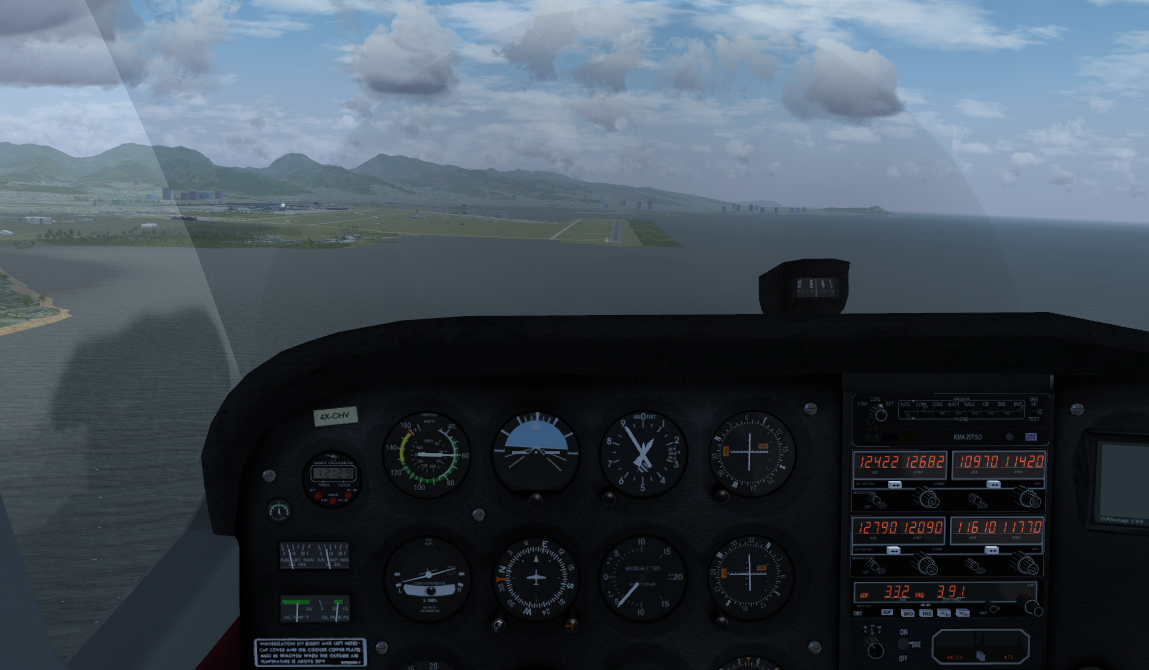
\includegraphics[width=\textwidth]{img/basic_tutorial/landing}
}

当飞机停住或者以慢速前进时,放开 \key{b} 键并增加一点发动机动力,以便滑行到停机位或机库。

\subsection{关闭发动机}\index{关闭}

\begin{itemize}
  \item 设置驻留刹车,按 \key{B} 键。
  \item 油门慢车(按住 \key{PageDown} 键一会)。
  \item 将油气混合比杆拉出,切断油路(正常模式下用鼠标点油气混合比杆左侧就可以将其拉出)。
  \item 将磁电机点火开关转到 OFF 位(按几次 \key{\{} 键)。
\end{itemize}

\subsection{复飞}\index{中止}

在降落时你需要时刻准备,因为状态不好或外部因素而中止降落,比如:

\begin{itemize}
  \item 塔台的指令
  \item 错误的速度或降落角度,因为已没有时间来修正
  \item 强劲的阵风
  \item 跑道上出现飞鸟
\end{itemize}

要中止降落,将油门推到最大(按住 \key{PageUp} 键),抬升机头以便爬升,当爬升姿态建立以后,收起襟翼。

降落要比起飞困难很多,在一个大型机场的跑道降落比如 KSFO(旧金山国际机场),要比小一点的跑道比如 KHAF(半月湾机场,在 KSFO 西南 10 英里处)要困难。

要练习降落,可以使用下面的命令行选项,启动模拟器并飞向跑道。飞机会被置于跑道外 5 英里处,高度 \textbf{1500} 英尺,速度 120 节。

\command{fgfs -$ $-offset-distance=5 -$ $-altitude=1500 -$ $-vc=120 -$ $-timeofday=noon}

使用 65 节而不是 70 节进近落地会让短跑道降落更容易。然而也需要更高超的控制技巧,因为更接近失速速度。因此与 70 节时很不同。

\section{关于风的问题}
\label{sec:Fwsw}

设想一个热气球,它在一个巨大的空气立方体里。也许这个空气立方体相对地面以高速运动,然而热气球却在立方体里纹丝未动。无论风速如何,在热气球里的人根本感觉不到一丝风。

同样道理,飞机在周围气团里飞行与在一个巨大的空气立方体里飞行是一样的。这个空气立方体相对地面的运动对飞机并没有影响。

你,飞行员,则不同。你更关心周围空气相对地面的速度。因为这个可以让你向左或向右偏移,又可以影响你更早或更晚的抵达目的地。

如果风与你飞行的方向相同,风就会把自身的速度叠加在飞机的空速上。因此相对地面你会更快,将更早抵达目的地。

反之当风从机头向机尾方向吹的时候,风会抵消飞机的空速,结果相对地面你变得更慢。会晚于预期抵达目的地,也让你有更多时间欣赏风景。

以上两种情况很好理解,更复杂的则是当风从侧面吹来的时候。来看下面的图表。

\begin{itemize}
    \item 下图中的 a 表示无风。飞行员想要抵达北面绿色的山丘。他可以直接航向山丘朝向正北,之后就会抵达。若没有风,你只需要将机头指向你的目的地即可。
    \item 下图中的 b,飞行员还是将飞机航向正北。然而却有左侧的来风,也就是从西面。飞机会被吹到右侧偏离航线。
    \item 下图中的 c,飞行员保持机头指向山丘。他虽然会抵达,但飞机会飞曲线路径。这会浪费一些时间。同时这样的曲线路径会在精确导航时变得很可怕。
    \item 下图中的 d 表示了最优的方式来抵达山丘。飞机指向山丘的左侧,稍微偏西也就是来风方向。这会抵消掉风的影响并让飞机直飞山丘。
\end{itemize}

\centerline{
  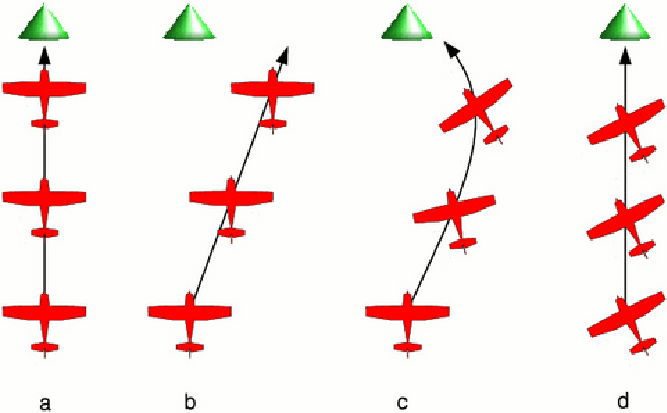
\includegraphics[width=0.65\textwidth]{img/basic_tutorial/wind-force}
}

飞机向左或向右偏航多少度?严肃的飞行员会使用几何和三角函数来计算正确的角度。粗略飞直线时你不需要计算。简单方法是瞄准你要飞行的点,注意它怎么移动。你会意识到自己漂移到了左侧还是右侧。然后让本能驱使你慢慢将飞机指向左或右,来抵消这股漂移的力量。刚开始你可能需要思考一下,很快这就会变成本能,就如同之前你学习如何直飞一样。你就不会一直让飞机指向目标,而是让飞机飞向目标。

飞的越快,风偏修正就越小。

\subsection{侧风起飞}
\label{sec:Swsw}

侧风起飞是很严峻的。因为机场设计时都会避免这种情况,会让跑道与盛行风平行。很多机场都会有多条跑道,这样做的目的是尽可能让跑道与风平行。

顶风起飞会让飞机更容易起飞,因为机翼与相对空气的速度加快增加了升力。当无风的时候,飞机必须加速到 55 节来起飞。也就是如果有 10 节的顶风,飞机就已经有了 10 节的空速,这时候只要加速到相对地面 45 节时就可以起飞,也就是缩短了起飞滑跑距离。

正如顶风会缩短滑跑距离,顺风则会增加距离。哪怕只是一两节的差距,就会产生滑跑距离上的巨大差异。几乎所有跑道都可以从两侧起飞,你可以很容易的从跑道另一侧起飞,并找到顶风。

要想获得风向和风速,最好是跑去询问塔台或者通过无线电询问之。另一个必要且备份的工具是跑道两旁的风向袋\index{风向袋 Windsock}。可以指示风速和方向,如果风向袋变得越来越直越来越硬,说明风速越大。下图里的风向袋表示风速 5 节:

\begin{center}
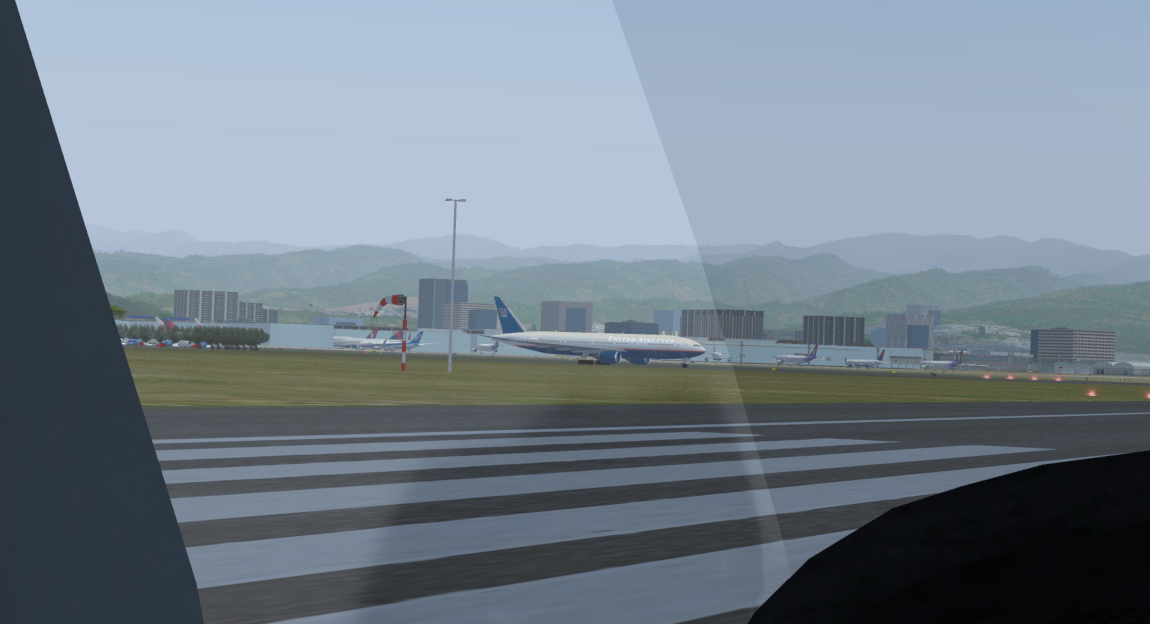
\includegraphics[width=\textwidth]{img/basic_tutorial/windsock-5kts}
\end{center}

不幸的是,机场跑道并不总是正对风,你需要在侧风中起飞。

技术上说与正常起飞只有两点不同:
\begin{itemize}
    \item 在起飞滑跑阶段,飞机会像风向标一样偏转。你需要用方向舵来修正,也许会需要方向舵有较大的角度来保持对准跑道。你需要在整个起飞过程里都保持方向舵。
    \item 起飞以后,飞机会因为方向舵的影响而转弯,你需要使用副翼来修正。当飞机升入空中以后,你可以适当减小方向舵和副翼,然后再对风进行修正。正如上文所述对准跑道。
\end{itemize}

\subsection{侧风降落}
\label{sec:Lwsw}

侧风降落与起飞非常相似:

\begin{itemize}
    \item 修正侧风对准跑道
    \item 在刚开始拉平时,用驾驶盘让飞机平直,使用方向舵抑制飞机的偏航倾向。
    \item 飞机可能会一侧机轮先着地,用方向舵让飞机另一侧机轮着地。
\end{itemize}

相应的技术细节可以参考:
\weblong{http://en.wikipedia.org/wiki/Slip_landing}{slip landing}.
另一篇文章:
\weblong{http://en.wikipedia.org/wiki/Crab_landing}{crab landing}\footnote{现时,这两篇维基百科链接都会指向同一个页面。——译者注}

\subsection{在风中滑行}
\label{sec:Twsw}

10 节以下的风,对塞斯纳 172P 来说并不需要特别的处理。但突然增大的风会让飞机倾斜甚至将其掀翻。

若想模拟地面有风时的滑行,可以将模拟器配置比较大的风,比如 20 节。这样的风任何时候都足以将飞机倾斜甚至掀翻。一个微小的错误就可能让飞机失事。

总的原则是你必须\emph{向来风的方向压盘}。这需要用物理的原理做一点解释:

\begin{itemize}
    \item 当风从 12 点钟方向(正前方)吹来时,这比较合乎逻辑,向 12 点钟方向推驾驶盘,升降舵会让机尾稍稍抬起。这样可以防止飞机在风中被掀翻。
    \item 当风从 10 点钟方向(左前方)吹来时,将驾驶盘向 10 点钟方向推,这意味着升降舵几乎回中,同时左侧副翼向上而右侧副翼向下。这样会压住左侧机翼并抬升右侧机翼。同时这也是防止飞机被风吹翻最稳固的位置。
    \item 当风从 8 点钟方向(左后方)吹来时。你也许想将操作相反,以便让左机翼推向地面。因此你需要推杆到 4 点钟位置,错!保持驾驶盘在 8 点钟位置。右侧副翼向下的位置,它的作用与金属档板一样。同时还能增加右侧机翼的升力,这正是我们想要的。相应的左侧副翼向上也可以降低左侧机翼的升力。
    \item 当风从正后方吹来时,也就是 6 点钟方向。这时候拉驾驶盘(指向 6 点钟方向)。向上的升降舵会让尾翼向下推。而这也是最佳位置。因为强风会将尾翼推向地面。虽然这一点难以理解,但机尾设计时已经考虑到这一点。
\end{itemize}

如果想正对风移动,则需要更多发动机动力。而当风从后面吹来时,你也许根本不需要发动机动力。总是保持发动机在最低需求。

特别的,转弯时要特别慢。一次只做一点改动。慢慢移动并谨慎考量驾驶盘的角度,连续的对着风的方向推杆。连续的降低发动机推力。时刻注意使用刹车不要太猛,如果让飞机突然刹停,很可能恰好进入风将飞机吹翻的角度。

\section{自动驾驶仪}\index{自动驾驶仪}
\label{sec:Autopilot}

\begin{wrapfigure}{r}{0.35\textwidth}
  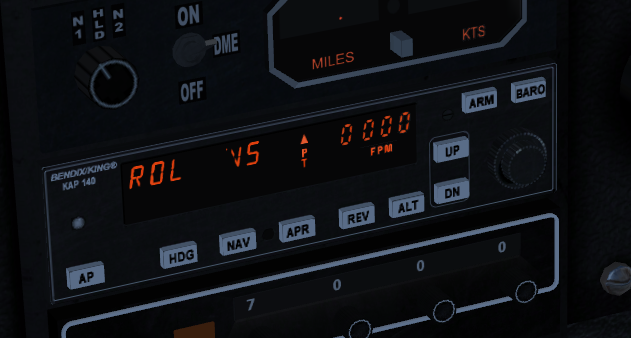
\includegraphics[width=0.35\textwidth]{img/basic_tutorial/autopilot}
  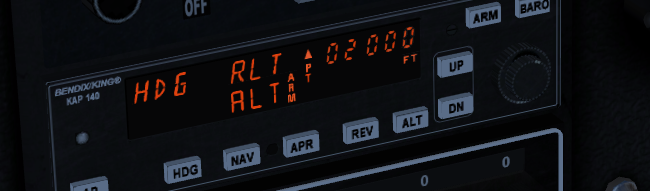
\includegraphics[width=0.35\textwidth]{img/basic_tutorial/autopilot-2}
\end{wrapfigure}

自动驾驶仪并不是一个“智能”的飞行员,它只能解决一些简单重复劳动。你作为飞行员必须一直关注一切动向。做好在其发生错误时关闭自动驾驶的准备,无论是在真实飞行还是模拟器里。

自动驾驶仪安装在驾驶盘的右侧。

按上面的 \button{AP} 按钮来启动。自动驾驶就开始控制飞机的横滚\index{自动驾驶仪!模式!横滚控制模式},让机翼保持与地平线平齐。如下图所示,自动驾驶仪上会有橙色的 \textcolor{orange}{\button{ROL}} 标识。要关闭自动驾驶再按 \button{AP} 按钮即可。

\index{自动驾驶仪!模式!航向模式}如果你按 \button{HDG} 按钮自动驾驶仪会让飞机飞向并保持某个航向,这个航向可以通过方位陀螺仪的红色游标来设定(详见 \ref{sec:Kierunek} 节)。\textcolor{orange}{\button{HDG}} 表示 Heading(航向)。再按一次自动驾驶仪上的 \button{HDG} 按钮会回到横滚控制模式(也可以用 \button{AP} 按钮关闭自动驾驶仪)。

\button{ALT}、\button{UP} 和 \button{DN} 按钮用来告诉自动驾驶仪,\index{自动驾驶仪!模式!垂直速率模式}要么控制垂直速率(\textcolor{orange}{\button{VS}}),要么控制高度并保持(\textcolor{orange}{\button{ALT}})。要了解更多塞斯纳 172P 自动驾驶仪的高级模式,可以参考此文档:\weblong{https://dealer.bendixking.com/servlet/com.honeywell.aes.utility.PDFDownLoadServlet?FileName=/TechPubs/repository/006-18034-0000_3.pdf}{Bendix King 的网站}

\section{然后呢?}
\label{sec:Poslowie}

此教程讲解了塞斯纳 172 的基本飞行方法。从这里你可以探索 \FlightGear{} 提供的更多特性。

当你掌握了此教程的内容以后,你可以看看本指南里的其他教程,比如飞向其他机场,天侯不佳时的仪表飞行以及直升机的飞行。

此教程略过了一些真实飞行员必须关心的问题:

\begin{itemize}
    \item 如何使用真实的检查单
    \item 如何在短跑道做紧急降落,以及发动机失效
    \item 如何依据大气规律、航图、法规、无线电信号和天气状况来导航
    \item 如何创建飞行计划,并按其精确飞行
    \item 如何放置人员、燃油和行李以得到正确的重心。
    \item 如何处理塔台和其他飞行器
    \item 如何处理多油箱及其系统
    \item 如何处理飞机各个系统的失效
\end{itemize}

此教程也没有涉及更高级飞机的特性,包括:

\begin{itemize}
  \item 起落架的收放
  \item 可变桨距的螺旋桨
  \item 多发动机
  \item 喷气式发动机
\end{itemize}

\section{鸣谢}

我想鸣谢:
\begin{itemize}
\item Benno Schulenberg 帮我纠正了此文中的英文错误
\item Albert Frank 告诉我大量飞行员的数据并修正了技术性错误
\item Vassilii Khachaturov 教会我有关 \FlightGear{} 的新特性
\item Dene Maxwell 有关在 Windows Me 下出现问题的处理
\item Mark Akermann 和 Paul Surgeon 感谢他们的备注
\item Michael ``Sam van der Mac'' Maciejewski 翻译了此教程的波兰语版本并将其用到了此指南里
\item \FlightGear{} 邮件列表里各位网友的热心帮助
\item \weblong{http://www.4p8.com}{4p8} 此教程使用了我朋友 Fr�d�ric Cloth 的网页空间
\end{itemize}

\section{其它机型}

我已经交叉检查了所有关于塞斯纳 172P 的数据,一个飞行员朋友证实了我并没有写太多垃圾,而且我在模拟器里也做了很多测试飞行。本节的内容基于我在模拟器里飞其它机型的经验,数据并不那么可靠。对于介绍相应的机型操作很有用,但仅仅满足基本飞行。

\subsection{如何降落 Cherokee Warrior II}
\label{sec:Cherokee}

Cherokee Warrior II 比塞斯纳 172P 更高级。因为其下单翼上反角设计在侧风时没有那么敏感。完全放出的襟翼提供了更多减速,并可让其在更短的距离内降落。

在 \FlightGear{} 里起飞和塞斯纳 172P 是一样的。在真实中,两者的检查单并不完全一样。

注意 Cherokee Warrior II 降落时有少许不同:

\begin{itemize}
    \item 平飞准备落地时,调整片必须稍微前推,以让驾驶盘处在中间位置。
    \item 最佳降落时的转速是稍稍低于转速表的绿色区域。大致保持表针竖直。
    \item 降落时只使用两档襟翼,不要收油门太多。
    \item 如果你保持两档襟翼降落,拉平和接地的过程与塞斯纳 172P 是一样的。然而三档襟翼会让空速显著下降,会快速接触跑道并很快停住。注意尽快降低前轮。(也可以在进近阶段使用三档襟翼下降,而不是收油门。在第二档向第三档襟翼过渡时开始对准跑道,不过保持两档襟翼并收油门似乎简单一些。一个有趣的特技玩法是平稳飞到跑道入口点,然后将发动机调到最低并放出三档襟翼。飞机几乎是直接落在跑道上。此方法很有趣但也能凑合\footnote{译者亲测,在 FlightGear 里若采用此法降落,需要较高的控制高度能力,否则很容易造成接地瞬间过高下降率(超过 300 英尺/分钟),有可能对机轮造成损坏。因此不建议采用此特技方式降落。——译者注})
\end{itemize}

在真实中,塞斯纳 172P 比 Cherokee Warrior II 更有优势的是油箱靠近机翼中间并高于发动机。另外还有一个自动油路转换开关。这意味着你不需要在飞行中关注燃油到发动机之间的问题。而 Cherokee Warrior II 的油箱是分离的,在两侧机翼并低于发动机。这意味着你需要在飞行中要不断切换两个油箱,如果一个油箱比另一个油箱轻,则会造成飞机的不稳定。而低于发动机则需要你来控制燃油泵和备用燃油泵。

一些链接:
\begin{itemize}
    \item \web{http://en.wikipedia.org/wiki/Piper\_Cherokee}
    \item \web{http://freechecklists.net/Resources/Piper/PA-28-151+Warrior/} \footnote{此链接也很有用 \web{http://wiki.flightgear.org/Piper\_Cherokee\_Warrior\_II} ——译者注}
\end{itemize}

\subsection{如何起降 Piper J3 Cub}
    \label{sec:PiperJ3}

Piper J3 Cub 与塞斯纳 172P 和 Cherokee Warrior II 有很大的不同。塞斯纳 172P 和 Cherokee Warrior II 的起落架是前三点式(也就是前机轮在主机轮的前面),而 Piper J3 Cub 是后三点式的飞机(主机轮在前)。后三点式飞机在起飞和降落时更困难。跑道上滑跑起飞时,你需要更加稳健的使用方向舵踏板。Piper J3 Cub 是介绍后三点式飞机最好的机型,合适的流程可以更简单的起飞和降落。失速速度略微低于 40 mph(此飞机空速以 mph 来表示)(大概 27 节)。起飞低于 50 mph。

我在飞 Piper J3 Cub 时的经验是向后完全拉杆,同时发动机油门推到最大。当前轮离地以后,再慢慢将驾驶盘回中。后面就和正常起飞一样了。然后让飞机加速到 50 mph。然后控制驾驶盘让飞机略高于 50 mph 来爬升。

降落流程与 172 很不一样,因为这架飞机没有襟翼,而且非常轻。

\begin{enumerate}
    \item 500 英尺高度并保持“恰好” 52 mph 速度对准跑道。让发动机盖子对准跑道入口,此时发动机盖子会完全挡住跑道。要想看跑道的位置,慢慢推杆然后再拉回正常。
    \item 当跑道入口对准仪表板的位置时(如果你的视线可以穿过仪表板),收油门到几乎最低并开始向跑道入口俯冲。使用驾驶盘保持 52 mph。如果你发现自己即向错过跑道边缘则稍稍推油(注意一股小风都可以对 Piper J3 Cub 产生较大影响)。
    \item 拉平并让发动机置于最低。不要拉的太猛,让机轮首先接触跑道。
    \item 当机轮接触跑道以后,\emph{推杆}以便让后轮悬空。你也许会想螺旋桨会撞到跑道,而飞机也会翻过来并损坏吧。然而一切都还 OK。机翼的负角度会让飞机慢下来(不要在其他机型上如此推杆,即便外形与 Piper J3 Cub 很相似。这样做会导致翻覆)
    \item 驾驶盘已经推到最大,此时按住鼠标左键控制方向舵,让飞机在跑道中线滑行。这并不简单,一个窍门是不要在飞机刚刚向左转的时候就说飞机已经向左转了。
    \item 当速度已经很低(方向舵控制也稳定了),你会看到后轮会落到地上。松开鼠标左键并回到驾驶盘控制模式,并将驾驶盘完全向后拉。机尾接触地面而机头抬高。现在你可以使用机轮刹车(按 \key{b} 键)(如果使用刹车太早,机头会撞到地面)。
\end{enumerate}

上面所述的起飞流程与第一降落流程对应。还有一个第二起飞流程与第二降落流程对应,然而我并没有成功,所以也没写出来。

 \subsection{如何起降喷气式飞机}
    \label{sec:Jet}

起飞喷气式飞机很简单,但你必须有快速反应能力。在 FlightGear 下我最喜欢的喷气式飞机是 A-4 Skyhawk。在 Linux 下可以使用命令 \command{--aircraft=a4-uiuc},前提是它已经安装了。

下面是一个“简朴的”起飞流程:
\begin{itemize}
    \item 按 \key{h} 键两次以打开红色并全屏化的 HUD\index{平视显示器}\index{HUD!全屏模式}。油门显示在 HUD 的最左侧。
    \item 空速表在仪表板左上部以“KIAS”表示。你也可以使用 HUD 上的空速指示。
    \item 将油门推到 $1\over2$ 位置。
    \item 保持驾驶盘在其后拉行程 $1\over2$ 的位置(如下图所示,图中线右侧的红色箭头)

        \begin{center}
		      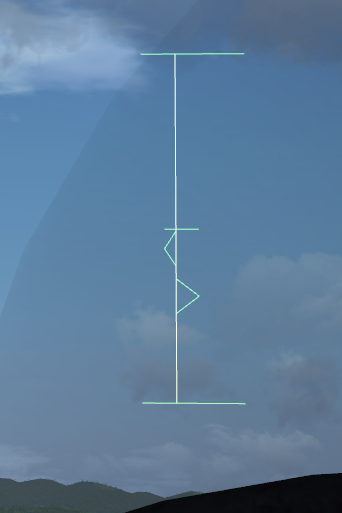
\includegraphics[width=0.35\textwidth]{img/basic_tutorial/hud-yoke-up}
	      \end{center}

   \item 不需要一定用方向舵以保持跑道方向,因为飞机会在其偏离跑道前起飞。(为了“安全”起见,还是要保持在跑道中线的,但对初学者来说用方向舵会很忙碌)
   \item 超过 160 节,飞机会抬起前轮,此时立刻拉操纵杆到中立位或稍向后,这会让飞机稳定在空速 200 节(这会让飞机平滑的爬升),我也不知道为何是 200 节,对真实 A-4 来说是不是正确。而我更希望使用 AOA(见下文)。
   \item 按 \key{g} 键收起起落架。
   \item 保持 $1\over2$ 的发动机推力,或者 200 节来穿过云层。或者收油到 $1\over4$ 左右来正常飞行(当然你可以用全发动机推力飞行,更有乐趣)。
\end{itemize}

更“紧张”的起飞流程与此相似,不同的是,使用全部发动机推力。飞机爬升很快而且你需要更陡峭的爬升角度以维持 200 节。也需要更快的收起起落架。

降落喷气式飞机和小型螺旋桨飞机方法不一样。通过在网上找到的一些文章,这是我的降落方式:

\begin{itemize}
    \item 距离跑道很远,保持 2000 英尺高度 200 节速度。然后放下起落架(按 \key{G} 键)并放出全部襟翼(总共三档,按三次 \key{]} 键)。
    \item 稳定保持 1000 英尺并准确减速到 150 节。使用升降舵控制高度,使用油门控制速度(与塞斯纳正好相反)
    \item 尝试对准跑道
    \item 如何知道何时必须开始向跑道俯冲呢?你需要使用\Index{HUD};完整的 HUD 有很多特性。如下图。当你看到“0”线与跑道入口之间的“距离”,是“0”线与“$-10$”点线之间距离的 25\% 时。说明可以开始俯冲。瞄准跑道入口处(下图的“距离”大概 64\%,距离降落还很远)。

\begin{center}
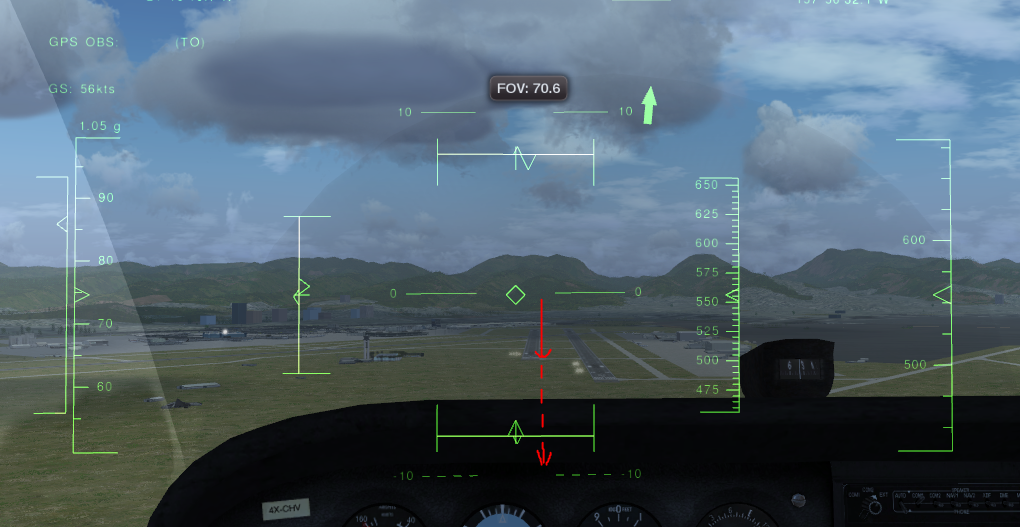
\includegraphics[width=\textwidth]{img/basic_tutorial/HUD-landing}
\end{center}

让我们来解释一下,两条标示为“0”的水平线段标示地平线。也就是水平线的位置,如果地球是平的。当你眼睛对准这两条“0”线时,你的目光是水平的。现在观察“$-10$”的虚线,这表示理想水平线下 10\textdegree{} 的位置。也就是说:当你看着目标“隐藏”在“0”线以下时,你需要把目光降低 10\textdegree{} 看“$-10$”的虚线处的“隐藏”物体。说个很重要的比喻,如果有个人在划船,位于“$-10$”虚线的位置。他如果要看你的飞机,需要抬起头 10\textdegree{}。也就是说他看到你的飞机处在地平线上 10\textdegree{} 的位置。如上图所示,跑道入口在红色“$-10$”虚线的 64\% 的位置。这就意味着你需要降低视线 6.4\textdegree{} 以看到跑道入口点,也就是下降角度需要 6.4\textdegree{}(太陡了)。所以 \Index{HUD} 可以帮助你测量下降的角度。喷气式飞机需要 2.5\textdegree{}(最大 3\textdegree{})的下降角度,也就是距离“$-10$”虚线 25\%(最大 30\%)。

\begin{center}
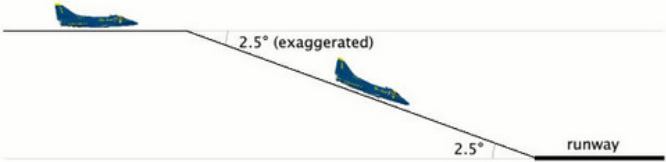
\includegraphics[width=0.5\textwidth]{img/basic_tutorial/glideslope}
\end{center}

\item 开始下降到跑道,使用驾驶盘保持对准,使用油门杆保持 150 节速度。
\item 注意理想水平线与跑道入口之间的角度,必须保持在 2.5 度(25\% 的 10\textdegree{} 线)
\begin{itemize}
\item [$\circ$] 若角度高于 2.5\textdegree{},说明你高于下降路径,你需要更快的下降高度。同时降低发动机动力并降低机头。
\item [$\circ$] 若角度低于 2.5\textdegree{},说明你低于下降路径,我不会说让你增加高度,而是你不要降低高度太快。同时增加发动机推力并稍抬机头。
\end{itemize}

\item 当非常接近跑道入口时,不要拉平,不要像塞斯纳 172P 那样拉杆。只需要让飞机高速接触地面,让飞机砸在跑道上。也就是说三个机轮几乎同时落地。然后将发动机收到慢车(如果你尝试通过拉杆让飞机悬停在跑道,会让机头猛然抬高,如果是 F-16 上会刮到机尾,有可能造成损坏)。

\item 按住 \key{b} 键并使用方向舵让飞机对准跑道。只需要很小的方向舵移动,否则飞机有可能会侧翻。
\end{itemize}

在真实中,HUD 会提供一个指示飞机移动的游标。会如下图所示,当你在一个固定高度飞行,此游标会在理想水平线上。当你下降对准跑道入口,你需要将此游标对准跑道入口,这会很容易并精确对准跑道(FlightGear 里的 HUD 中间有一个菱形标志,有时也很有帮助,但目的不一样。它表示了飞机机头的指向。比如当你以较低的速度向地面下降,游标应该指向地面,然而 FlightGear 的菱形会指向空中。另外 B-52 上的 HUD 有速度游标,在降落时很有用)。

\begin{center}
	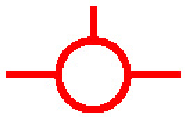
\includegraphics[width=0.25\textwidth]{img/basic_tutorial/aim-point}
\end{center}

同样在真实中,HUD 还会有一条 -2,5\textdegree{} 线来协助找到正确下降角度。只要将此线保持在跑道入口即可。

此外关于空速,快速的军机依赖于使用迎角。迎角(AoA)是机翼与相对气流之间的锐角。保持最优的迎角降落有个好处是不用依赖于飞机的配载,就如同最优的空速一样。为了保证每次落地的迎角都是正确,你需要保持正确的空速,无论配载如何。

迎角也在 HUD 上显示出来了,如下图的三个灯。当上部的 $\vee$ 亮起,表示你的迎角太大,需要向下俯。当下面的  $\wedge$ 亮起表示迎角太小,需要向上抬头。中间的 $\bigcirc$ 表示迎角正好。显然,俯仰会影响到下降率,你需要同时配合油门的调节。

\centerline{
  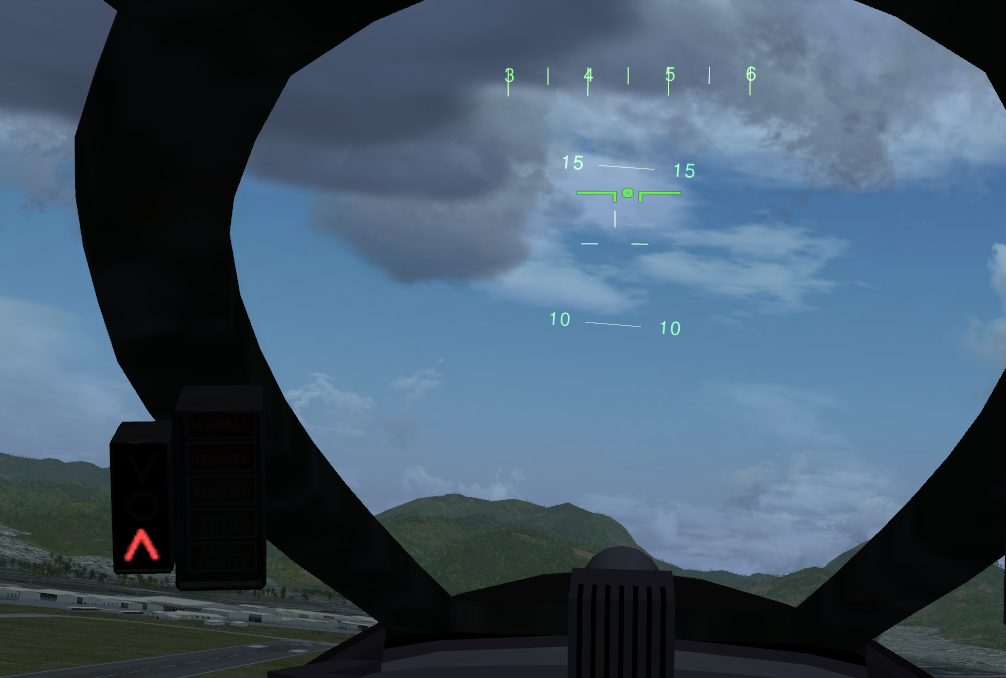
\includegraphics[width=0.5\textwidth]{img/basic_tutorial/f-14b-hud}
}

塞斯纳 172P 和 A-4 Skyhawk 是两个极端,大多数飞机都在这两个极端之间。如果你能够掌握这两种飞机(和一两种后三点式飞机),你将会明白大多数飞机的起降。

160 节对 F-16 来说是很合适的降落速度,当然也需要飞机落在跑道的一瞬间,调整油门让发动机到最低转速,否则会错过跑道。不用考虑襟翼,貌似它们会在起落架放下时自动放出(参考 \ref{sec:Stall} 有关失速的讲解)。

对虚拟的波音 737 来说,140~150 节以及全部 8 档襟翼全部放出可以很好的降落。然而不要盲目相信我,因为我只有很少的经验,也没有搜索专业的数据。落地速度与载重相关,我猜 140 节是空载。波音 737 貌似需要柔和的拉平,拉平操作要更早\footnote{参考波音 737 手册,正常降落速度在 135~150 节之间,襟翼 25 度,而不是全部放出。在距地面 50 英尺左右开始拉平,并柔和收油门到慢车。——译者注}。

讲解塞斯纳 172 和 A-4 Skyhawk 的起飞流程时,我建议你将升降舵拉到其 $1\over2$ 的位置。不过对于 Pilatus PC-7 并非如此,保持升降舵回中。让飞机加速到 100 节,然后柔和拉杆。降落开始对准跑道时,放出全部襟翼不要收油门。当越过跑道入口以后,再收油门。看起来 100 节是很好的降落速度。

塞斯纳 310 也是如此,跑道加速时最好保持升降舵回中。飞机会因为你放出的一档襟翼自己抬起机头。如果你一直保持驾驶盘后拉,机头会快速仰起而你也会面对可怕的俯仰问题。

很多虚拟的飞机,比如大型航线客机或快速飞机,需要快速的物理计算。然后需要在命令行加入 \command{--model-hz=480} 参数。如果发现飞机不太容易降落,可以尝试使用这个选项。

降落塞斯纳 172P 的时候,其实角度比喷气式的 2.5\textdegree{} 要陡。当然你可以在小角度落地,前提是跑道前方地形允许。或者作为乘客你的耳朵会对压力比较敏感……

\subsection{如何起降 P-51D “野马”}
\label{sec:P-51D}
你有机会驾驶一架 \weblong{http://en.wikipedia.org/wiki/P-51_Mustang}{P-51 “野马”}吗?也许不会。其实此飞机的起降很危险。你需要很多训练,而当 P-51D “野马”升入空中以后就没什么危险了。它很容易驾驶。

在中低高度,P-51 不会好过“喷火”和梅塞施密特战斗机。最大的不同在高空。当敌机窜入高空以后,P-51 可以保持效能和机动性。另一个不同,P-51 有很好的流线型外观,因此可以比“喷火”飞的更远。这两大不同,使得 P-51 可以为轰炸机远程护航,让轰炸变得更有效率也能有效打击纳粹。

要在 Linux 下启动 P-51D “野马”可以使用命令行参数 \command{--aircraft=p51d}

在 \FlightGear{} 里起飞 P-51D,襟翼放出一档。将操纵杆完全向后拉,发动机推到最大,并按住鼠标左键控制方向舵,以保持在跑道上。一旦你达到 100 mph,突然将方向舵向右蹬全程的 1/3。快速松开鼠标左键并推杆以抬起尾轮(不要推太多,恰好将尾轮抬起即可)。现在保持鼠标左键放开,只在必要时对方向舵做调整。在大概 150 mph 的时候拉杆让飞机爬升。不要忘记收回起落架和襟翼。

转弯时不要太陡,你可能会失去控制并坠机。

要降落,放出全部襟翼并放下起落架。130 mph 看来很不错,最大 140 mph。从 1000 英尺开始进近并以低角度俯冲,就如同喷气机。当进入跑道以后,完全关闭发动机(按 \key{\{} 键)。不要飞过跑道。尽快将机轮落在跑道上(就像喷气机)。使用方向舵让飞机沿跑道中线。当后轮落在跑道上时,柔和拉杆以便让机尾紧贴跑道。继续使用方向舵控制飞机,现在机尾已经在地面上了。按需使用刹车。

\subsection{如何起降 B-52 “同温层堡垒”}
    \label{sec:B52}

\FlightGear{} 里的 B-52F 非常成功,也是我最喜欢的飞机。B-52F 和塞斯纳 172P 的不同主要有:
\begin{itemize}
    \item B-52 起动时需要设置停留刹车并放出襟翼。
    \item 襟翼只有两种状态:收起和放出。放出意味着机翼上更多升力,而不是减速。如果你想减速,需要使用绕流板,它们在机翼上方。按 \key{k} 键升起绕流板,按 \key{j} 键收起。绕流板有七块。
    \item 塞斯纳 172P 的主机轮有两个,飞机两侧一边一个。为了让机轮同时落地,你需要保持机翼与地面平行。B-52F 的主机轮有前后两套。而为了让所有这些主轮落地,你需要让机体与地面平行。
 \end{itemize}

这是我的 B-52F 起飞流程:
\begin{itemize}
    \item 将驾驶盘\emph{推}到全部行程 $1\over3$ 的位置。
    \item 发动机推到最大推力
    \item 松开停留刹车(按 \key{B} 键)
    \item 按住鼠标左键控制方向舵,以让飞机在跑道中线
    \item B-52F 需要全部跑道来起飞(KSFO)。
    \item 当 B-52F 离开地面,大概 190 节就可以很好的飞到一定高度了
    \item 收起襟翼和起落架。
\end{itemize}

要降落,B-52 的 HUD 已经提供了飞机形状的游标,正如我在上面喷气机那一节里说的。你只需要将那个图标对准飞机的中间。并保持低于理想水平线 2.5\textdegree{} 的位置。130 节到 140 节看起来很适合降落。保持迎角在 3\textdegree{},我必须承认我倾向使用速度控制,而不是迎角控制。如果飞机在 130~140 节,只需让飞机“砸”在跑道上。否则如果速度太快,拉平以后飞机飘的距离会增加。刹车看起来很有效果(按 \key{b} 键)。它们可以让 B-52 像塞斯纳 172P 那样在跑道上快速停下。

飞行重放看起来是很明智的。可以用来检查机体降落时是不是与地面平行。还可以坐到乘客座椅上,来比较和航线飞行时你作为乘客的感受。按 \key{K} 键可以显示飞机在空中的虚拟航迹。

B-52 造成的事故可能因为:
\begin{itemize}
    \item 转弯太陡,机翼几乎擦碰到地面.
    \item 让飞机恢复水平,飞机反应太慢。因此你会发现转弯会超过预期。
    \item 做了太极端的操作:蹬方向舵到极值,与当前转弯方向相反,这会让飞机瞬间从空中跌落。
\end{itemize}    


%%%%%%%%%%%%%%%%%%%%%%%%%%%%%%%% ENGLISH VERSION %%%%%%%%%%%%%%%%%%%%%%%%%%%%%%%%%%%%%%%%%%%%%%%
\iffalse
\section{The First Challenge - Flying Straight}
\label{sec:FlyingStraight}

Once \FlightGear{} is started you will see the following window and hear the
sound of an engine:

\begin{center}
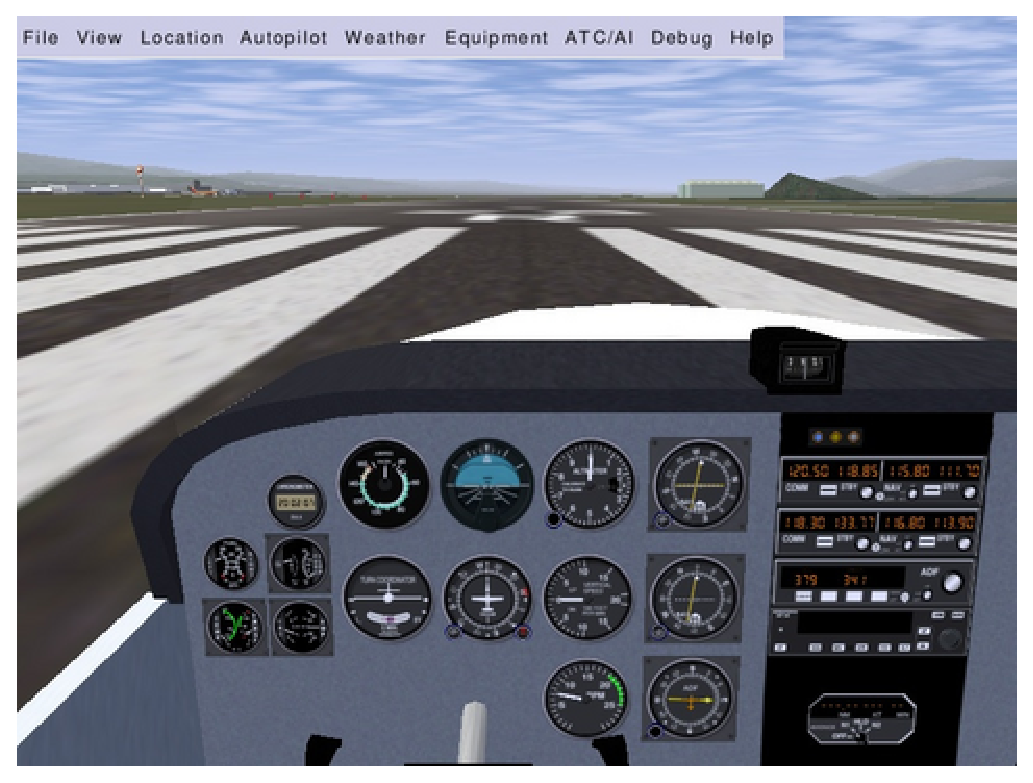
\includegraphics[width=0.5\textwidth]{img/tut_6}
\end{center}

On startup, the aircraft is at the end of the runway with the engine running
at low power. The airplane will occasionally tremble a little, but it won't
move.

\subsection*{About the keyboard.}\index{keyboard}

\begin{itemize}
    \item In this tutorial, a lowercase key letter indicates you should simply
  press that key. An uppercase means you must press shift and that key.
  (The \textcolor{blue}{\key{$\Uparrow$~Shift}} keys are those two keys with
  a hollow fat arrow pointing upwards.) In other words: if you are told to type
  ``v'', simply hit the \key{v} key briefly.
  \index{keyboard!uppercase and lowercase keys} If you are told to type ``V'',
  press the \key{Shift} key down and while you have it pushed down, hit the
  \key{v} key, then release the \key{Shift}  key. (In short: V is the same as
  \key{Shift-v}.)
    \item The tutorial will assume you have the \key{NumLock} switched on.
  \index{keyboard!numeric} When switched on, you should find a small green
  light on at the right of your keyboard. Press the
  \textcolor{green}{\key{NumLock}} key repeatedly until the lamp is on.
\end{itemize}

\begin{center}
\includegraphics[width=0.5\textwidth]{img/tut_7}
\end{center}

\index{view!changing}
Press \key{v}, to view the aircraft from the outside. Type v repeatedly to
scroll through a number of different views until you return to the cockpit.
Typing \key{V} will cycle backwards through the views.):

\begin{center}
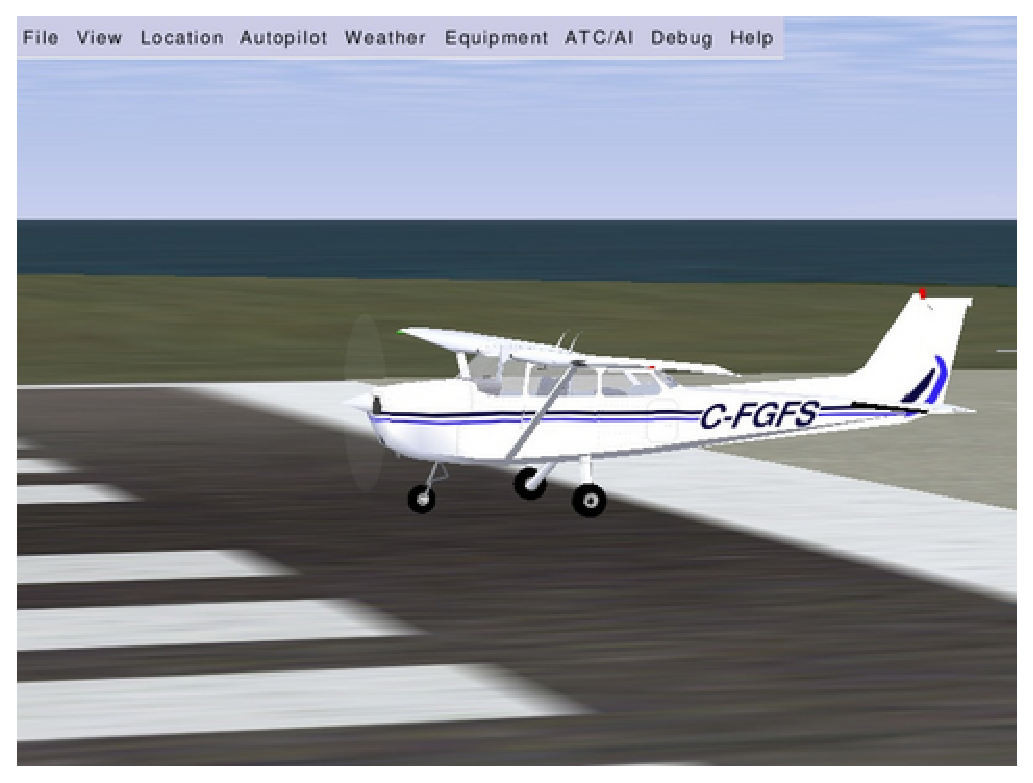
\includegraphics[width=0.5\textwidth]{img/tut_8}
\end{center}

In real life, we would have inspected the airplane all around to check
everything is working, nothing is hampering the moving parts,
and nothing is obstructing the instrument openings. In the simulator, this is
already done for us before we start.

Hold the \key{Page Up} key down for about eight seconds. You will
hear the engine sound rise.

The airplane will start accelerating down the runway. As it does so, it will
drift to the left, before finally taking off, banking to the left,
falling to the ground and crashing (probably).

\index{view!instant replay}
You can see a replay of the crash using the  \button{View -> Instant Replay}
menu. Click the \button{Replay} button at the bottom of the dialog window, then
use \key{v} and \key{V} to see the airplane from the outside. The
picture below shows the end part of the flight. You can take a snapshot by
typing the \key{F3} key.
You can also use the \key{F10} key to toggle the menu bar on or off.

\begin{center}
\includegraphics[width=0.5\textwidth]{img/tut_9}
\end{center}

Having observed your crash, exit from \FlightGear (using \button{File->Quit})
and restart the simulator using the same options as before.

In order to fly straight you need the airplane's control\index{yoke} yoke:

\begin{center}
\includegraphics[width=0.5\textwidth]{img/tut_10}
\end{center}

You can control the yoke using a joystick, or by moving the mouse. To use the
mouse you need to be in mouse yoke mode. Get in that mode by pressing \key{Tab}.
The mouse cursor becomes a $+$ sign. Move the mouse and see the
yoke moving accordingly. Type \key{v} to see the plane from the outside. If you
move the mouse again you will see the tail elevator and the ailerons at both
wings ends move. If your viewpoint is too far from the aircraft to see any
movement, type \key{x} a few times to zoom in.
Type \key{X} to zoom back out. \key{Ctrl-x} returns the view to the default zoom
level. Type \key{V} to change the view back to the cockpit.

Pressing \key{Tab} again gets you in mouse view mode. In this mode the mouse cursor will
be a $\leftrightarrow$. sign. This allows you to look around easily by moving
the mouse. Clicking the left mouse button will re-center the view.  You can also
change your view direction in the normal and yoke modes by holding down the right
mouse button and moving the mouse. A further press of \key{Tab} will return you to the
normal mouse mode.

To summarize, the \key{Tab} key cycles the mouse through three modes:
\begin{itemize}
    \item \textit{Normal mode}\index{mouse!normal mode}. This mode allows you to
  click on the menu and on the instrument panel.
    \item \textit{Yoke mode}\index{mouse!yoke mode}.\index{yoke!mouse yoke mode}
  The mouse controls the yoke (+ pointer shape).
    \item \textit{View mode}\index{mouse!view mode}. The mouse controls the
  view direction ($\leftrightarrow$ pointer shape).
\end{itemize}

Try taking off again using the mouse to control the yoke. Press \key{Tab} to put
the mouse in yoke mode ($+$pointer shape) and raise the engine throttle to
maximum by holding the \key{Page Up} key down. Do not try to keep the airplane
rolling straight on the runway using the mouse/yoke. Let it drift leftwards.
Wait till it rises in the air. Then use the mouse to try and get the
airplane to fly straight. (If you want to control the airplane on the
ground see section \ref{sec:TaxiTurning}.)

You will find that you must prevent the airplane from banking to the left:

\begin{center}
\includegraphics[width=0.5\textwidth]{img/tut_11}
\end{center}

... or to the right:


\begin{center}
\includegraphics[width=0.5\textwidth]{img/tut_12}
\end{center}

... or from plunging to the ground:


\begin{center}
\includegraphics[width=0.5\textwidth]{img/tut_13}
\end{center}

Try to fly more or less straight, with the horizon stable slightly above the
airplane nose:

\begin{center}
\includegraphics[width=0.5\textwidth]{img/tut_15}
\end{center}

Whatever your skills at video games or simpler simulators, you will probably
not succeed at first. The airplane will crash, probably quite soon after
take-off. This is the moment where most candidates get desperate and abandon
trying to fly a simulator or a real aircraft. Just hold tight and keep trying.
Eventually you will develop a feel for the subtle control inputs required.

\index{yoke!pulling}
The most common error is moving the mouse forwards to bring the nose up. In
fact, you must pull the yoke by moving the mouse backwards to do this.

Equally, when you want to lower the airplane's nose, you must move
the mouse forwards. This can seem odd, but all airplane control yokes
are designed that way. With time, you will wonder how you every thought it
worked any other way. \index{troubles!mouse speed} You will also find that
small mouse movements have a large effect on the aircraft. You may find that
decreasing your mouse sensitivity may help initially.

If you have difficulty visualising this, the following analogy may help.
Imagine a soccer ball is on your desk and you have ``glued'' your hand
to the top of it. If you move your hand forwards the ball will roll forwards
and your fingers will point to to the desk. If you move your hand backwards the
ball will roll  back and your fingers will now point up at the ceiling.
Your hand is the airplane:


\begin{center}
\includegraphics[width=0.5\textwidth]{img/tut_6}
\end{center}

Another common error is the assumption that the control inputs directly
match airplane bank. In other words, you believe if the control yoke is
level, the airplane will fly level. This is not true. The yoke
controls the \emph{rate} at which the airplane banks. If the airplane is
banked 20\textdegree{} to the left and the control yoke is level, the
airplane will stay banked at 20\textdegree{} left until some other force
affects it. If you want to return the airplane to level flight, you have to
turn the control yoke slightly to the right (move the mouse slightly
rightwards) and keep it slightly to the right for a while. The airplane
will turn slowly rightwards. Once it is level with the horizon, bring the
control yoke level too. Then the airplane will stay level (until some other
force changes its orientation).

A third error is trying to find ``the right position'' for the
yoke/mouse. Naturally, you will want to find the fine tuning that will leave
the airplane fly straight. Actually there is no such ideal yoke
position. The airplane is inherintely unstable in the air. You must constantly
correct the airplane's attitude and keep it flying straight with tiny movements
of the mouse. This may seem to take all your concentration intially,
but just like driving a car, keeping the aircraft straight and level will soon
become second nature. For longer flights, you will eventually use the autopilot
to keep the airplane level, but this is outside the scope of this tutorial.

To help fine-tune your senses to the control inputs required, keep your eyes on
the outside scenery and not get fixated on the instruments or the yoke. Check
the angle of the horizon and its height above the airplane's nose. The horizon
line and the airplane engine cover are your main flight instruments. Look at
the instrument panel only once in a while.

While the mouse is in yoke\index{yoke!mouse yoke mode} control mode
($+$ pointer shape), don't move it close to the FlightGear window
edges. Once the mouse leaves the window, it stops controlling the aircraft,
often at the worse possible moment!
If you wish to use the mouse outside of the window, first go back to standard
mouse mode by pressing \key{Tab} twice.

You can also control the yoke using the four \key{keyboard arrow} keys
or the keypad \key{8}, \key{2}, \key{4} and \key{6} keys. While initially this
may seem easier than the mouse, you cannot make the very fine adjustments
required for accurate flying, so it is much better to persevere with the mouse.

You may hear beeping sounds while flying around the airport. These are
landing aid signals\index{landing!aid signals}. Don't worry about them for the
moment.

You will know that you have mastered this when you can make the aircraft climb
steadily in the air. The next step is to learn to keep the aircraft at a
constant altitude, or to make it ascend or descend slowly and under your
control.

Keeping the aircraft at a constant altitude involves observing the altimeter
and making small changes with the mouse forwards or backwards to stop the
aircraft ascending or descending respectively.

\index{altimeter} The altimeter instrument is at the middle top of the
instrument panel. The long needle shows hundreds of feet, the short needle
shows thousands of feet. The altimeter below shows an altitude of
300 feet, approximately 100 meters.


\begin{center}
\includegraphics[width=0.25\textwidth]{img/tut_17}
\end{center}

As you ascend or descend the altimeter will change accordingly, turning
anti-clockwise as you descend, and clockwise as you gain height. If you see
the altimeter ``unwinding'' you will be able to tell that you are losing height
and move the mouse backwards slightly to raise the nose.
After a while you will notice that when flying level the nose of the aircraft
is always in the same position relative to the horizon. This is the aircraft
attitude for level flight. By putting the nose in that same position, you will
achieve almost level flight without having to reference the instruments. From
there you can fine-tune your altitude.

Beware: an altimeter does not automatically show the absolute altitude
above sea level\index{altitude!absolute}. You must adjust for the local air
pressive. The little black knob on the lower left side of the
altimeter\index{altimeter!tuning} allows you to adjust the altimeter. Start
\FlightGear{} and stay on the ground. Click (in normal mouse mode) inside the
black knob. A click on the left half makes the altimeter turn back. On the
right half the altimeter turns forward. Use that little knob to tune in the
current altitude. The principle is you use the knob when you are sure about
the altitude. If you know you are at 1,100 feet altitude, tune in 1,100 feet
on the altimeter. Clicking with the middle mouse button makes the knob
turn faster, or you can use the scrollwheel on your mouse.
Type \key{Ctrl}-\key{c} to see the two button halves highlighted.

To make settings the altimeter easier, airports advertise their altitude in
various ways. They may provide a radio service (called ATIS in the USA)
to broadcast the current air pressure at sea level. This is expressed in
inches of mercury. The altimeter contains a small scale inside which is
calibrated in this way. You can set your altimeter using this scale.
Alternatively, if you are on the ground and know the altitude of the airport,
you can simply adjust your altimeter until it displays the correct altitude.

\begin{center}
\includegraphics[width=0.25\textwidth]{img/tut_18}
\end{center}

Note that there is an important difference between ``altitude above sea
level'' and ``altitude above the ground''. If you fly near Mount Everest at an
altitude of 24,000 feet above sea level (AMSL), your altitude above the ground
(AGL) will be much less. Knowing the altitude of the ground around you is
obviously useful.

\section{Basic Turns}
\label{sec:InFlightTurning}

While if you had enough fuel you could return to the same airport by flying
straight head for thousands of miles, being able to change direction will
make your flying more enjoyable and useful.

Once you are able to fly more or less straight, it is time to
learn to turn. The principle is simple:
\begin{itemize}
    \item When the airplane is banked to the left, it turns to the left.
  \item When the airplane is banked to the right, it turns to the right.
\end{itemize}

\begin{center}
\includegraphics[width=0.25\textwidth]{img/tut_19}
\end{center}
\index{turn coordinator}

\index{turn coordinator} To turn, you do not need high levels of bank.
20\textdegree{} is more than enough for a safe and steady turn. The turn
coordinator indicates your angle of bank by showing a depiction of your aircraft
from behind. The picture below shows the turn coordinator when the airplane is
banked 20\textdegree{} to the right. You can also tell the bank angle by
observing the angle of the horizon.

Try the following: keep the airplane banked around those 20\textdegree{} for a
few minutes and keep your eyes outside the aircraft You will see the same
ground features appear again and again, every 120 seconds. This shows you
need 120 seconds to make a 360\textdegree{} turn (or 60 seconds for a
180\textdegree{})turn). This is particularly useful when navigating.
Whatever speed the airplane is flying, if you bank at 20\textdegree{} you
always need 60 seconds to make a 180\textdegree{} turn in the Cessna 172P.

So, by banking the airplane to the left or to the right, you make it turn to
the left or to the right. Keeping the airplane level with the horizon keeps
it flying straight.

The little purple ball in the bottom of the turn indicator
shows the sideways forces. In real life you would feel these as your turn,
however it is not possible to simulate these, so you must simply keep an eye
on the ball. If you turn neatly (using the rudder a little bit),
the ball will remain centered. If the ball is pushed say rightwards, this
means you the pilot too are pushed rightwards. Like in a car turning to the
left. During a neat turn in an airplane, even a strong turn, the passengers
never endure a sideways force. They are only pushed a little harder on their
seats by the centrifugal force.

By experimenting you will notice you can make much steeper turns by
banking the airplane to high angles and pulling back on the yoke. Turns at over
60\textdegree{} bank angle are the realm of aerobatics and military flying, and
dangerous is aircraft such as the Cessna.

\section{Taxiing on the ground}
\label{sec:TaxiTurning}

While \FlightGear{} starts you by default conveniently lined up on the
runway and ready to go, you may be wondering how to get your aircraft from
its hangar, along the taxi-ways to the runway. This is taxiing.

The picture below shows the \index{tachometer} instrument. It displays how fast
the engine is turning in hundreds of revolutions per minute (RPM).

\begin{center}
\includegraphics[width=0.25\textwidth]{img/tut_20}
\end{center}

Type the \key{Page Up} key a few times,
until the tachometer is showing 1,000 RPM (as shown above). If required
type the \key{Page Down} key to decrease the engine speed.

At roughly 1,000 RPM, the airplane will move forward on the runway, but it will
not accelerate and take off.

\index{brakes!right wheel [.] (dot)} Type the ``\key{.}''key (\key{Shift-;} on
Azerty keyboards). The airplane will make a sharp turn to the right. If you
keep the ``\key{.}''key down the airplane will halt. When you type the
``\key{.}'' key, you are activating the brake on the right wheel of the
airplane.

\index{brakes!left wheel [,] (colon)} To activate the brake on the left
wheel, use the ``\key{,}'' key.

\index{brakes} The ``\key{,}'' and ``\key{.}''  keys simulate two brake pedals
located at your feet on a real airplane. Using the throttle and the brake pedals
you can control the speed of the aircraft and cause it to turn on the ground.

The brakes can be very useful when taxiing slowly on the runway. You can also
steer the nose-wheel of the aircraft. In a real airplane this is done by pushing
the rudder pedals with your feet. You push with your feet on the side you want
to turn towards. If you don't have real rudder pedals, there are two ways to
control the virtual rudder pedals:
\begin{itemize}
    \item Using the keypad  \key{0} and \key{Enter} keys
  \index{rudder!keyboard control}. If you type the keypad \key{Enter} key say
  seven times, you will see the airplane firmly turns to the right and
  stays turning that way. Type the keypad \key{0} key seven times to get the
  airplane back rolling (almost) straight.
    \item Using the mouse. While the mouse is in yoke control mode
  ($+$ pointer shape), if you hold the left mouse button down, the mouse
  controls the rudder pedals instead of the yoke. The rudder pedals are
  connected to both the rudder \index{mouse!rudder control}
  \index{rudder!mouse control} and nose-wheel. This method is much more precise.
\end{itemize}

Start the simulator, Type \key{v} or \key{V} to view the airplane from
the outside and keep \key{x} down a couple of seconds to zoom in on the
airplane. Look at the front wheel and keep keypad \key{0} down. Then
keep keypad \key{Enter} down. See the front wheel turn. Press \key{Tab}
to get in yoke control mode ($+$ pointer shape).
Keep the left mouse button down to get in rudder control mode and move
the mouse to the left and to the right. Note that the rudder, that big
vertical control surface at the rear of the plane, moves together with
the front wheel.

I tend to control the rudder pedals using the mouse while the front
wheel is on the ground and use the keypad \key{0} and \key{Enter}
keys once it has lifted off. In other words: I
keep the left mouse button down while the front wheel is on the
ground. This allows for a precise and easy rudder control on the
ground. Then I simply release the left mouse button once the front wheel
lifts off.

\begin{center}
\includegraphics[width=0.5\textwidth]{img/tut_23}
\end{center}

\subsection{Airspeed}

Just like driving a car, it is good to know how fast you are traveling.
The aviation equivalent of a speedometer is the airspeed indicator (ASI),
calibrate in nautical miles per hour (knots).

\begin{center}
\includegraphics[width=0.25\textwidth]{img/tut_24}
\end{center}

A knot\index{speed!units!knot [nautical mile per hour]} is 1.85325
kilometer/hour. So, if you want to have a rough idea of your speed in
flight expressed in km/h, multiply the knots displayed by 2. A knot is
1.15115 miles per hour, so very roughly, 1 knot is 1 mph. Note that some
aircraft ASIs (in particular the Piper J3 Cub) display mph instead of knots.

The airspeed indicator displays the speed of the aircraft compared
to the surrounding air, not the speed compared to the ground like a car
speedometer does. If the plane is halted on the ground and there is
a 10 knot wind blowing from straight ahead, the airspeed indicator will
display 10 knots airspeed, although the plane will not be moving relative to
the ground.

When the airplane rolls over the runway at more than 40 knots, you must
prevent the front wheel from touching the ground. The nosewheel is not designed
for high speeds and in real life would shimmy and wear out.

During take off, once over 40 knots you can make the front wheel leave the ground by pulling back
gently on the control yoke. Don't turn sharply at high speed on the ground.
Doing so may cause the aircraft to tip over.

The picture below shows the front wheel slightly lifted. Don't overdo
this. Keep the airplane's white nose cover well below the horizon. You
just need to lift the plane's nose very slightly.

\begin{center}
\includegraphics[width=0.5\textwidth]{img/tut_25}
\end{center}

Question: if the front wheel no longer touches the runway, how do you
steer the airplane? Answer: still using the rudder pedals. As mentioned above,
the rudder pedals are linked to both the nose-wheel and the tail rudder, that
big vertical moving part at the tail of the plane:

\begin{center}
\includegraphics[width=0.5\textwidth]{img/tut_26}
\end{center}

At airspeeds above 40 knots, the rudder has enought air-flow over it to steer
the airplane.

Note the front wheel and the tail rudder don't make the airplane turn
at exactly the same rate. So when the rudder takes over the front wheel,
you must adapt the rudder pedals angle. That means fast typing keypad
\key{0} and keypad \key{Enter} (or hold the left mouse button down and
tightly control the rudder with the mouse).

Once you've become familiar with the nose-wheel and rudder, you can use these
new controls to keep the airplane straight on the runway during take-off.

Say the airplane is heading too much to the right. You type
keypad \key{0} a few times to make it turn back to the left. Don't
wait till the aircraft has straightened up completely. Type keypad \key{Enter}
before the aircraft reaches the direction you wish to travel. Otherwise you will
find that you will over-correct and have to turn back again. If you use the
mouse, such corrections are much easier and more precise.

To summarise: two methods exist to steer the airplane on the ground: the
differential brakes on the side wheels and the rudder pedals. This
control redundancy is very common in aviation. If one method fails,
you still have another method available to perform the task.

You may be wondering why the aircraft drifts to the left when it rolls on the
ground, forcing your to compensate with a little push on the right rudder
pedal? The main reason is the flow of air produced by the propeller. It
blows along the airplane body, but also corkscrews around the airplane
fuselage. The upper part of that slight vortex pushes the vertical tail
to the right. This causes makes the front of the aircraft to yaw to the left.

You can center all yoke and rudder controls by typing \key{5} on the
keypad. This is a good preflight precaution. Sometimes it can ``save
your life'' in flight if you find yourself with controls all over the place!

\section{Advanced Turns}
\label{sec:Turning}

As with turning on the ground, there are two methods of turning in the air.
You can use the wing ailerons (steered by the yoke/mouse) as described above or
you can use the tail rudder (steered by the rudder pedals / the
keypad keys /\key{0} and \key{Enter}.

Why two ways? Partially for redundancy, but mainly because they are
complementary. The main effect of the rudder is yaw (rotation around the
vertical axis), while the main effect of the ailerons is roll (rotation around
the longitudonal axis).

\begin{itemize}
    \item When flying close to the ground, it is better not to bank the
  airplane in order to turn. The rudder is used more instead. Acting on the
  rudder pedals allows you to turn the airplane without excessive banking.
    \item When the plane is just above the runway, the two side wheels need to
  be at the same height above the runway for landing. That means the wings
  must be level with the horizon. The plane is not allowed to bank. You keep
  the plane wings level with the horizon by using the yoke/mouse/ailerons.
  Note this does not need to be perfect. A bank of a few degrees is harmless.
    \item In flight, especially at high speed, the rudder is an in-efficient
  way to turn the aircraft:
\begin{itemize}
    \item It causes the airplane to present its flank to the airstream, increasing
  drag.
    \item The airplane turns very slowly.
    \item You will lack control while turning.
    \item At high flight speed the centrifugal force will be disturbing or even
  dangerous.
\end{itemize}
Using the yoke/mouse/ailerons allows for efficient, fast, reliable and
comfortable turns.
  \item The rudder can be vital when the wings are stalled. Indeed, during a
  stall the wing ailerons become less effective or even useless.
  (Note that some airplanes can go in a very dangerous stall if you overdo the
  rudder control at low speed.)
\end{itemize}

When you turn in flight, using the ailerons, you still need the rudder
a little bit. You add a little bit of rudder. This allows you to
compensate for the adverse yaw created when you roll using the
ailerons. In a real aircraft, you can feel this sideways motion. In the
simulator, you can check this visually on the turn coordinator. In the
picture below the little ball is pushed rightwards during a strong turn
to the right using the ailerons. That means you the pilot endure a rightwards
force too. You can compensate this by pushing the right rudder pedal
(type the keypad \key{Enter} key a few times). In normal flight you should use
the rudder to keep the little ball centered.

\begin{center}
\includegraphics[width=0.25\textwidth]{img/tut_27}
\end{center}

So, in normal flight use the ailerons to turn, while close to the ground at low
speed use the rudder. However, one method never completely cancels out the
other. You still need the rudder at high altitudes and speeds. Reciprocally you
have to use the ailerons a little bit when close to the ground, to keep the
wings level with the horizon.

Even when taxiing, you should use the ailerons. Otherwise, strong winds can
blow the aircraft onto its side. To counteract this, your should turn the
ailerons into the wind. This raises the aileron in the wind, helping to
keep the wing down.

You should avoid making quick and agressive movements of the rudder. On the
ground at high speed this can make the airplane turn too sharply. In flight
at low speed it can cause a very dangerous type of stall. In flight at high
speed it can cause all kinds of aerodynamic and physical discomfort.
Instead, make gentle movements of the rudder.

I recommend you practise turning with the rudder in flight. Fly at a low
speed of about 70 knots. Try to keep the altitude stable by increasing
and decreasing the engine power. Use the rudder to turn towards a ground
feature and maintain a heading, then turn the aircraft towards a new heading.
See how the plane yaws. Learn to anticipate rudder
control. Don't try to make steep turns. Use the yoke/ailerons to keep
the wings level constantly.

\section{A Bit of Wieheisterology}

Wieheisterology comes from the German phrase ``Wie hei\ss t Er'' --
``What's that name''. This section is about gauges, switches and controls of
the aircraft. While in the simulator you can take off and land a basic airplane
with just the engine throttle and the yoke, but you will need all the controls to
perform securely and efficiently.

\subsection{Engine control}
\label{sec:EngineControl}

An airplane engine is designed for simplicity, reliability and efficiency.
Rather than use advanced electronic ignition and fuel injection systems found in
modern cars, they instead use older technology that doesn't rely on electrical
power. That way, the plane can still fly even if it suffers complete electrical
failure.

\subsection*{Magneto}\index{magneto}

On the bottom left, below the instrument panel you will find the
magneto switch and engine starter:


\begin{center}
\includegraphics[width=0.25\textwidth]{img/tut_28}
\end{center}

To see the switch, either type  \key{P} to get the schematic instrument
panel or type \key{Shift-x} to zoom out (\key{x} or \key{Ctrl-x} to
zoom back in).

You can move the switch with the \key{\{} and \key{\}} keys (use the \key{Alt
Gr} key on Azerty keyboards).

You are probably aware that the fuel inside a car engine is ignited by
electric sparks. Modern car engines use electronic ignition. An airplane engine
uses a more old-fashioned (but more reliable) magneto ignition instead. For
redundancy, it contains two such magnetos: the ``left'' one and the ``right''
one. When you change the magneto switch on OFF, both magnetos are switched off
and the engine will not run. With the magneto switch on L you are using the
left magneto. On R you are using the right magneto. On BOTH you use both.
In flight you will use BOTH.

Given that you use both magnetos in flight, why have the switch? The reason
is that during your pre-flight checks you will verify that each of the magnetos
is working correctly. To do this, increase the RPM to about 1500 then switch
the magneto switch to L and observe the tachometer. You should observe a
slight drop in RPM. If the engine cuts out, the left magneto is broken. If
you do not see an RPM drop, then the switch may be faulty, as both magnetos
are still switched on. You can then perform the same test on the right magneto.
Of course, in the simulator, the magnetos are unlikely to fail!

Should one of the two magnetos fail in flight, the other one will keep the
engine running. The failure of one magneto is rare, the failure of both
simultaneously is almost unheard of.

You may have typed \key{\{} to shut the engine down. To start
the engine again after doing so, type \key{\}} three
times in order to put the magneto switch on BOTH. Then use the starter motor
by pressing the \key{s} for a few seconds, till the engine is started.

You can also turn the magneto switch and start the engine by clicking
left and right of the switch in normal mouse mod). Type \key{Ctrl-c} to
see the two click sides highlighted by yellow rectangles.

If you turn the switch to OFF, the engine noise stops. If you quickly
turn the switch back to L, the engine starts again as the propeller is still
turning. If you wait for the propeller to stop, placing the switch on L, R
or BOTH won't start the engine. (Once the engine is halted, always place the
magneto switch to OFF.)

\subsection*{Throttle}\index{throttle lever}

\begin{center}
\includegraphics[width=0.25\textwidth]{img/tut_29}
\end{center}

You already know that you increase the engine power by pushing that throttle
rod in (\key{Page Up} key). You decrease the power by pulling the
control out (\key{Page Down} key). You can also click left and right of
the lever (middle mouse button for quicker moves, \key{Ctrl-c} to
highlight the left and right halves).

What does ``increase the power'' actually mean? Does it mean you increase
the amount of fuel delivered to the engine? Yes, but this is not enough to
fully understand what you are doing. You need to be aware that the engine is
also fed with a huge amount of air. The engine's cylinders burn an
\Index{mixture} of fuel and air. Fuel alone wouldn't burn.
Only a mixture of fuel and air can detonate and move the engine
pistons. So when you push the throttle in, you increase both the fuel
and the air fed to the engine.

\subsection*{Mixture}\index{mixture}

The amount of air compared to the amount of fuel is critical. The
proportion of the two has to be tuned closely. This is the purpose of
the mixture lever. The picture below displays the mixture lever, pulled out far
too much.

\begin{center}
\includegraphics[width=0.25\textwidth]{img/tut_30}
\end{center}

When the \index{mixture!lever} mixture lever is fully pushed in, you
feed the engine with an lots of fuel and little air. This is known as a
``rich'' mixture. When the lever is pulled out completely, there is an
excess of air, known as a ``lean'' mixture. The correct position to produce
maximum power is in between these two extremes, usually quite close to fully
pushed in.

When you start the engine and when you take off, you need a fuel-rich
mixture. That means the mixture lever should be pushed in. A fuel-rich mixture
allows the engine to start easily. It also makes the engine a little
more reliable. The drawback is that a part of the fuel is not burned
inside the engine. It is simply wasted and pushed out the exhaust. This makes
the engine more polluting, it decreases the energy the engine can deliver and
it slowly degrades the engine by causing deposits of residues inside the
cylinders.\index{mixture!optimisation}

Once in normal flight, you have to pull the mixture lever a little, to
get a more optimal mixture. Check this out by doing the following. Start
the simulator. Put the parking brakes on with key B (that is
\key{Shift-b}). Push the throttle in to its maximum. The engine RPM should
now be close to the maximum. Slowly pull on the mixture lever (using the
mouse in normal pointer mode). You will see the RPM increases a little.
You get more power, without increasing the fuel intake. You waste no
fuel and it pollutes less. If you continue to pull the mixture lever, the RPM
will decrease back away, because now there is too much air. The excess of air
slows the explosions down inside the cylinders and decreases the explosion
temperature, hence the thermodynamic yield decreases. You have to tune in the
optimal mixture. For thermodynamic reasons, the best mixture isn't exactly at
maximum power - it is better for the engine to be running very slight richer
or leaner than maximum power. This also avoids the possibility of the fuel
detonating explosively damaging the engine. You can find the
maximum power point by the fact you get the highest RPM. (Another method is to
check the engine exhaust temperature. Roughly, this is the point at which you
get the highest temperature.)

The mixture control allows you to burn less fuel for the same speed and
distance, and therefore fly farther and pollute less. However, if you
mis-manage it, it can cause serious problems.
Suppose you go flying at high altitude and pull out the
mixture lever accordingly. At high altitude there is less oxygen available
so the correct mixture will be quite lean - i.e. with little fuel being used.
Then you descend back in order to land. If you forget to push the mixture lever
in as you descend, The fuel/air mixture will become far too lean and the
engine will simply halt.

When landing, you have to tune back in a mixture that is a little too
rich in fuel. This means pushing the mixture lever in. That way the
engine becomes a little more reliable and will be better adapted to a
decrease in altitude.

I wrote above that placing the magneto on OFF is not the right way to
stop the engine. The right method is to pull the mixture
lever\index{engine!shut down}. First pull the throttle
out completely, to get the engine to minimum power and fuel
consumption. Then pull the mixture lever, till the engine stops because
the mixture contains too much air. This ensures the engine doesn't get
choked by waste fuel residues. Finally, turn the magneto switch to
OFF to ensure the engine won't start again accidentally.

An important warning: you may think the RPM indicator reflects the
engine power. Wrong. Two things make the RPM increase: the engine power
and the airplane speed. To check this, fly to a given altitude
then pull the engine power to minimum. Try out diving to the ground
then rising back to altitude. You will see the RPM varies significantly as does
your airspeed. It rises while diving and decreases while climbing.

One pitfall of this is when you intend to tune the engine power in for
landing. Suppose you're descending towards the airport,
flying fast. You know the ideal RPM for landing is around 1,900 RPM. So
you pull the throttle till you get 1,900 RPM. You think you tuned in
the appropriate RPM. You think you shouldn't bother any more about it.
But when you level off, the plane's speed starts to decrease, along with the
RPM. A few minutes later, you get the low flight speed you wanted. You don't
see the RPM is now far too slow. You will either lose altitude or
stall. Or both. Be cautious with the throttle and with the RPM
indicator. Either pull on the throttle more steadily or be mentally
prepared to push it back in quickly.

\subsection{Wings and speed}
\label{sec:WingsAndForce}

Say you are flying with full engine power. Dropping the nose a little makes you
lose altitude and raising the nose a little makes you gain altitude. You may
think this is quite straightforward. The plane travels in the direction it is
heading; the direction the propeller is heading. This is not the best way to
think about it.
This model would be fine for a rocket, but not for an airplane. A rocket is
lifted by its engine, while a plane is lifted by its wings.
That's a huge difference.

Get a big rigid square of cardboard, hold it horizontally in your hand
with your arm stretched out and make it do fast horizontal movements
while rotating your torso. When the cardboard moves flat through the
air, it experiences no lift force. If you twist your arm slightly to
give the cardboard a slight upward angle, you will feel it tends to
lift in the air. There is an upward force acting on the cardboard.
That's the way a wing holds a plane in the air. The wings have a slight
upward angle and lift the airplane. The more angle you give the
cardboard, the more lift force. (Till you give it too steep an angle.
Then you will rather feel a brake force. The cardboard is ``stalling''
(see below).)

\begin{center}
\includegraphics[width=0.5\textwidth]{img/tut_31}
\end{center}

\begin{itemize}
    \item When you pull the yoke, the airplane's nose rises up. Hence the wings
  travel through the air at a steeper angle. Hence the lift force on the
  wings is stronger. Hence the plane rises in the air.
  \item When you push the yoke, the airplane's nose dives. Hence the wings
  travel through the air with less angle. Hence the lift force on the wings
  decreases. Hence the plane descends.
\end{itemize}

What matters is the angle the wings travel through the air. This is the
angle of attack.

I wrote above that when the wings travel through the air with no angle of
attack, they don't produce lift. This is false. It would be true if the wings
were a flat plate like the cardboard. But they aren't. The wings are a
slightly curved airfoil. This makes them create lift even when traveling
through the air at no angle of attack. Actually, even with a little negative
angle of attack they still create a lift force. At high speed the airplane
flies with the wings slightly angled towards the ground!

\begin{center}
\includegraphics[width=0.5\textwidth]{img/tut_32}
\end{center}

The angle at which the wings travel through the air matters. Something
else matters too: the speed. Take the cardboard again in your hand.
Hold it with a given slight angle and don't change that angle. Move it at
different speeds through the air. The faster you move the cardboard, the more
upward force it experiences.
\begin{itemize}
    \item When you increase the engine power, the plane increases speed, the
  lift force on the wings increases and the plane gains altitude.
    \item When you decrease the engine power, the plane decreases speed, the
  lift force on the wings decreases and the plane loses altitude.
\end{itemize}

To make things a little more complicated: when rising in the air, the
airplane tends to lose speed. When descending, it tends to gain speed.

That's all a matter of compromises. If you want to fly at a constant
altitude and at a given speed, you will have to tune both the engine
power and the yoke/elevator (or better: the trim (see below)), till you
get what you want. If you want to descend yet keep the same speed, you
have to push the yoke a little and decrease the engine power. And so
on. You constantly have to tune both the engine power and the
yoke. However, during a normal flight you can simplify this by simply
choosing a comfortable engine power level then relying on the yoke and
trim for altitude.

A very interesting exercise you can perform with the simulator is to
fly straight with full engine power. Get maximum speed while keeping in
horizontal flight. Then decrease the engine power to minimum. Pull steadily
on the yoke to keep the plane at constant altitude.
The plane slows down steadily, meanwhile you have pull more and more on the
yoke to stay level. Since the speed decreases the lift from the wing
will decrease, but you compensate the loss of speed by increasing the wing
angle of attack. This proves the plane does not necessarily travel in the
direction its nose is heading. In this experiment we make the nose rise
in order to stay at constant altitude. Once the plane is flying very slowly,
and the nose is very high, you may hear a
siren yell. That's the stall warning (see below). This indicates that the angle
of attack is too high for the airfoil to produce lift. The wings are
no longer producing lift and the plane quickly loses
altitude. The only way to correct this is push the yoke forwards to reduce the
angle of attach, making the nose drop, then apply full power to gain speed and
finally bring the yoke carefully back to level flight.

Question: is it better to control the airplane's speed and altitude
with the yoke or with the throttle? Answer: it depends on what exactly
you intent to do and on the situation you are in. In normal flight, as
said above, you tend to set a comfortable engine power level, forget
about it and rely on the yoke and trim. During take off and landing the
procedures are quite strict about the use of yoke and throttle. You do
the opposite: control the speed with the yoke and trim, control the
altitude and descent speed with the engine throttle. This will be
discussed further below.

\subsection{The flaps} \index{flaps}
\label{sec:Flaps}

The flaps are situated at the rear of the wings, either side of the
aircraft fuselage.

\begin{center}
\includegraphics[width=0.5\textwidth]{img/tut_33}
\end{center}

You deploy the flaps and retract them back in by using the
\index{flaps!control lever}flaps control lever:


\begin{center}
\includegraphics[width=0.25\textwidth]{img/tut_34}
\end{center}

You can either click on it with the mouse or use the \key{[} and
\key{]} keys. Key \key{[} to retract the flaps one step, \key{]} to
deploy them one step at a time. Type \key{v} to view the plane from the outside
and try out \key{[} and \key{]}. (On the schematic instrument panel the
flaps lever is located at the lower right.)

In the Cessna 172P. there are four \index{flaps!steps}flaps settings:
\begin{itemize}
    \item 0\textdegree{} - for normal flight and normal take off.
    \item 10\textdegree{} - for short field take off, when you want to gain altitude while
  flying slowly. Or during the first stange of an approach to land.
    \item 20\textdegree{} - to slow the aircraft and lose altitude quickly, for example
  when descending towards the runway to land.
    \item 30\textdegree{} - To lose altitude even more quickly.
\end{itemize}

The flaps are somewhat delicate. Do not deploy the first step of flaps above
110 knots. Do not deploy the second or third stage of flaps above 85 knots.

The flaps create large amounts of drag on the aircraft and brake the plane at
high speed. This is one more reason not to forget to pull the flaps back in
once you fly above 85 or 110 knots.

To check the flaps position visually, either use the mouse view mode to look
at the back of the wing, or type \key{Shift}-\key{right arrow} to shift the
view to the right and then quickly \key{Shift}-\key{up
arrow} to get back to front view.

Flaps increase wing lift by altering the shape of the airfoil. The wing lifts
more at a given speed with the first stage of flaps set. Hence you will get in
the air a little sooner during take off. It also has the effect to make the
plane fly with a lower nose attitude. This is useful as it provides a better
view of the runway when taking off or landing.

The flaps also increase drag on the aircraft. The second and third stage of
flaps produce much more drag than lift, so they are used to brake the
plane. This is particularly useful when landing, because the airplane glides
very well. If you cut down the engine power completely, the plane will descend, yet
but too slowly. You need to deploy two or three flaps steps in order to
brake and really descend towards the ground.

The fact that the flaps brake during landing makes you need more engine
power during the landing. This can seem odd. Why not simply throttle
the engine down to minimum and use less flaps steps? The answer is that it is
better to have a strongly braking plane and lots of engine power,
as the plane reacts faster to your commands. Should the
engine fail, then just retract flaps as needed and glide to the runway.

\index{side-slip}
What can you do if you have full flaps extended and need to increase your
rate of descent further? Slowly push the rudder pedals on one
side. This will make the plane present its flank to the air stream and
brake. Compensate the turning by using the ailerons (yoke). This is known as
side-slipping, and is a very effective way to lose height progressively as it
is easy to stop at any point.

\subsection{The stall}\index{stall}
\label{sec:Stall}

An aircraft relies on the smooth flow of air over the surface of the wing to
produce lift. However, if the wing is at too high an angle of attack, this
flow is broken, and the wing no-longer produces lift. With no lift, the
aircraft cannot fly, and quickly drops back to earth. This is known as a stall.

A stall is an emergency situation, whatever the While it can happen at any
speed, it commonly occurs in slow flight. A given aircraft has a specific
stall speed, at which no angle of attack can produce enough lift. You should
always keep your aircraft well above the stall speed. To help, aircraft
are equipped with stall sirens that sound when the angle of attack is
approached.

If you encounter a stall, the remedial action is to immediately
drop the nose, and apply full power, bringing the nose level when flying
speed has been attained again. However, doing so will cause the aircraft to lose
altitude, which you may not have to spare when landing or taking off!

\index{spin}A spin occurs when one wing stalls before the other, which can
occur in a steep turn at low speed. As one wing is still flying, the aircraft
turns around the stalled wing, spinning tighter and tighter. To get out of a
spin, you need to apply rudder to straighten out the spin into a normal stall,
then recover as above.

Aircraft like the Cessna 172 and Piper Cub, have benign stalls, and are unlikely
to enter a spin. High performance jets, such as the F16 have much more agressive
stalls, and can easily enter a spin.

To practise this in the simulator, do the following:
\begin{itemize}
    \item Fly at constant altitude and attitude.
  \item Reduce engine power, raising the nose to avoid entering a descent.
  \item Continue to reduce power until the stall begins.
  \item Try to control the plane while it stalls and descends to the ground.
  \item Keep the yoke pulled to the maximum and the plane in a steady attitude,
  the wings parallel with the horizon. Try to change direction.
  \item Recover by lowering the nose, applying full power, and correcting the
  attitude once flying speed has been regained.
\end{itemize}

You can also experiment with stalls with different flap settings, and high speed
stalls by making abrupt attitude changes.

Experiment with different aircraft. Compared with the Cessna 172 the Cessna
Citation jet, stalls much more agressively and with little warning..

\subsection{The trim}\index{trim}
\label{sec:Trim}

The trim is the dark big vertical wheel with gray dots located at the middle
below the instrument panel:

\begin{center}
\includegraphics[width=0.25\textwidth]{img/tut_35}
\end{center}

On \FlightGear, the keys \key{Home} and \key{End} adjust the trim.
\key{Home} rolls the wheel upwards while the \key{End} rolls the wheel
downwards. You can also click on the upper or lower half of the trim wheel.

In first approximation, the trim does the same as the yoke: it acts on
the elevator. Turning the trim wheel downwards is the same as pulling
on the yoke. Yet there is a key difference between the trim and the
yoke. The trim remains in position after you make a change, while the
yoke only continues to affect the elevator while you apply pressure and
returns the elevator to neutral when you release it.

During cruise flight, the required elevator position to keep the aircraft at
constand altitude will not be completely neutral - it will vary depending on
the air outside the aircraft, the current fuel level, and the payload.
Obviously, holding the yoke continually to retain a constant attitude would
quickly become tiring. By using the trim to ``trim out'' the elevator force
required for cruise flight, the yoke can be kept neutral.

During take off the trim should be neutral. Otherwise you may find that it
either refuses to take-off with the normal level of yoke control, or takes off
too quickly.

During landing, try to get the yoke/mouse/elevator towards neutral position
by tuning the trim. This makes making small adjustments to your attitude and
position easier. On the Cessna 172p this means trim on neutral. On the
Cherokee Warrior II this means the trim a little ``pulled''.

The trim wheel movement is much slower than the yoke, allowing for delicate
changes in trim. Be patient.


\subsection{What direction am I flying?}
\label{sec:Kierunek}

Knowing the direction you are going is obviously a good idea. There are three
basic ways to determine the direction you are flying:
\begin{itemize}
    \item Look through the windows. If you are flying regularly from the same
  airport, you will learn to recognize the ground features such as roads, hills,
  bridges, cities, forests. In a simulator, you only have a narrow view of the
  virtual outside world. Several ways exist to allow you to pan your virtual
  head inside the airplane:
      \begin{itemize}
        \item Use \key{Shift} and the four arrow keys to
      look to the front, rear, left and right.
        \item Use \key{Shift} and the keypad keys to look in the
      four directions mentioned above and in four diagonal directions
      in-between.
        \item Hold down the right mouse button in normal or yoke mode and move
        the  mouse to change the view direction.
        \item Use the mouse in view mode (\key{Tab}, $\leftrightarrow$). This
      allows you to look in every direction, including up and down. Click the
      left mouse button to bring the view back to straight ahead.
    \end{itemize}
 \item The magnetic compass. This is located above the instrument panel. The
 compass is simple, but is affected by the acceleration of the aircraft, and
 magnetic abnormalities on the ground. Also, the compass points towards magnetic
 north rather than true north. This deviation varies depending on your location.

\begin{center}
\includegraphics[width=0.25\textwidth]{img/tut_36}
\end{center}


  \item The directional gyro (picture below) or ``heading indicator''. The
  gyro is powered by a vacuum system. The gyro is set to match the magnetic
  compass, and is not affected by magnetic issues, or aircraft movement.
  However, due to gyroscopic precession and friction in the instrument, over
  time it drifts and must be reset by reference to the magnetic compass on
  ocassion. To reset the HI, during cruise flight, use the black knob on the
  bottom left of the instrument
  (normal mouse pointer mode, click left or right half of the knob, middle
  mouse button to move faster, \key{Ctrl}-\key{c} to highlight halves).
  (The red knob, bottom right, is used to tell the autopilot what direction
  you wish to fly (\textcolor{red}{\button{HDG}} = ``heading'').

\begin{center}
\includegraphics[width=0.25\textwidth]{img/tut_37}
\end{center}

\end{itemize}

\subsection{A look around the panel}

Finally, let's have a look at the instrument panel, combining the instruments
described above with some new ones.

\subsubsection{The six-pack}

Let us start with the most important instruments any simulator pilot must know,
these are known as the ``holy six'' or the ``six-pack''
.
In the center of the instrument panel (Fig.\,5), in the upper row, you will
find the \Index{artificial horizon} (\Index{attitude indicator}) displaying
\Index{pitch} and \Index{bank} of your plane. It has pitch marks as well as
bank marks at 10, 20, 30, 60, and 90 degrees.

Left of the artificial horizon, you'll see the \Index{airspeed indicator}. Not
only does it provide a speed indication in knots but also several arcs showing
characteristic \Index{velocity rages} you have to consider. At first, there is
a green arc indicating the normal operating range of speed with the \Index{flaps}
fully retracted. The white arc indicates the range of speed with flaps in action.
The yellow arc shows a range which should only be used in smooth air. The upper
end of it has a red radial indicating the speed you must never exceeded,
unless you want to break up the plane in mid-flights\ldots

Below the airspeed indicator you can find the \Index{turn indicator}. The
airplane in the middle indicates the roll of your plane. If the left or right
wing of the plane is aligned with one of the marks, this would indicate a
standard turn, i.e. a turn of 360 degrees in exactly two minutes.

Below the plane, still in the turn indicator, is the \Index{inclinometer}. It
indicates whether the \Index{rudder} and \Index{aileron}s are co-ordinated.
During turns, you always have to operate \Index{aileron} and \Index{rudder}
in such a way that the ball in the tube
remains centered; otherwise the plane is skidding. A simple rule says:
``Step on the ball'', i.e. step onto the left rudder pedal when
the ball is on the left-hand side.
\medskip

If you don't have pedals or lack the experience to handle the proper
ratio between aileron/rudder automatically, you can start \FlightGear{}
with the option \texttt{-$ $-enable-auto-coordination}.\index{auto
coordination}

To the right-hand side of the artificial horizon you will find the
\Index{altimeter} showing the height above sea level (not ground!) in hundreds
of feet.  Below the altimeter is the \Index{vertical speed indicator}
indicating the rate of climbing or sinking of your plane in hundreds of feet
per minute. While you may find it more convenient to use than the altimeter
in certain cases, keep in mind that its display usually has a certain time-lag.

Further below the vertical speed indicator is the propellor tachometer, or RPM
(rotations per minute) indicator\index{RPM indicator}, which displays the
rotations per minute in hundreds. The green arc marks the optimum region for
cruise flight.

The group of the main instruments further includes the \Index{gyro compass}
being situated below the artificial horizon. Besides this one, there is a
\Index{magnetic compass} sitting on top of the panel.

Four of these gauges being arranged in the from of a ``T'' are of special
importance: The air speed indicator, the artificial horizon, the altimeter,
and the compass should be scanned regularly during flight.

\subsubsection{Supplementary Instruments}

Beside the six-pack, there are several supplementary instruments. To the very
left you will find the \Index{clock}, obviously being an important tool
for instance for determining turn rates. Below the clock there are
several smaller gauges displaying the technical state of your engine.
Certainly the most important of them is the \Index{fuel indicator} - as
any pilot should know.

The \Index{ignition switch} is situated in the lower left corner of the
panel (cf. Fig.\,4). It has five positions: ``OFF'', ``L'', ``R'',
``BOTH'', and ``START''. The first one is obvious. ``L'' and ``R'' do
not refer to two engines (as the Cessna 172 only has one) but the
two magnetos, providing redundancy in the case of a failure.. The two switch
positions can be used for test puposes during preflight. During normal
flight the switch should point on ``BOTH''. The extreme right position
is for \index{starting the engine} using a battery-powered
\Index{starter} (operated with the ``s'' key).

The handle below the yoke is the parking brake. In the vertical position,
the parking brake is ON. The parking brake is operated with the ``B'' key.

\subsubsection{Radios}

The right hand side of the panel is occupied by the \Index{radio stack}. Here
you find two \Index{VOR} receivers (NAV),\index{NAV} an \Index{NDB} receiver
(\Index{ADF}) and two \Index{communication radio}s (COMM1/2)
\index{COMM1}\index{COMM2} as well as the autopilot.

The \Index{communication radio} is used for communication with \Index{air
traffic facilities}; it is just a usual radio transceiver working in a special
frequency range. The frequency is displayed in the LEDs. Usually
there are two \Index{COM transceiver}s; this way you can dial in the frequency
of the next controller to contact while still being in contact with the previous
one.

The COM radio can be used to listen to the current weather conditions at an
airport, known as ATIS. To do this, simply dial in the ATIS frequency of the
relevant airport. You can find this by selecting \texttt{ATC/AI->Frequencies}
from the menu, and selecting the 4-letter ICAO code of a nearby airport.

Each COM radio has two frequencies configured - an `active' frequency which
the pilot is transmitting and receiving on, and a `standby' frequency which may
be changed. In this way, you can continue to listen on one frequency while tuning
another one.

You can change the radio frequency using the mouse. For this
purpose, click left/right to the circular knob below the corresponding
number. The corresponding switch left to this knob can be used for
toggling between the active/standby frequency.

Use of the autopilot and radio navigation equipement is covered in later
tutorials. For the moment you can ignore these radio instruments as
long as you are strictly flying according to \Index{VFR} (\Index{visual
flight rules}).

\section{Let's Fly}

By now you will be able to keep on runway while
taking off by using the rudder and you're able to fly straight, descend, climb
and make gentle turns. This section will describe a slightly more realistic
approach to taking off and landing, and introduce some of the more subtle
concepts you should be aware of.

\subsection{A realistic take off}
\label{sec:Start}


The following general rules apply during a normal take-off:
\begin{itemize}
    \item The nose-wheel should be lifted from the runway at approximately 40
  knots.
  \item Immediately after take-off, you should accelerate to 70 knots, to stay
  well above stall speed, in case of a gust of wind, or engine failure.
  \item Don't fly much above 75 knots to ensure you gain height as quickly as
  possible.
  \item Follow the runway heading until at 500 feet. This way, if you suffer
  an engine failure, you can easily land back on the runway you left.
  \item Don't over-fly buildings until at least 1,000 ft.
    \item Close to the ground, turns should be gentle and well coordinated
  using the rudder.
\end{itemize}

So, you need to take off and rise in the air at a steady speed of around
75 knots. However, when you raise the nose slightly at 40 knots, the aircraft
will probably take-off at around 55 knots. To accelerate quickly to 75 knots,
lower the nose slightly immediately on take-off, then raise it once 75 knots
has been achieved. You are using the yoke to control the speed of the aircraft.

Putting this all together with what you have learned previously, a normal
take-off using the mouse will consist of the following:

\begin{enumerate}
  \item Adjust the altimeter to the correct altitude, based on the airport
  altitude. For reference, KSFO is at sea level - 0ft.
    \item Check aileron and elevator are neutral by observing the yoke position.
  \item Change the mouse to control mode by pressing \key{Tab}.
  \item Hold the left mouse button down to control the rudder.
  \item Apply full power (hold \key{PgUp} until the throttle is fully in).
  \item As the aircraft accelerates down the runway, keep it in the center by
  making small adjustments using the mouse.
  \item As 40kts is reached, release the left mouse button, and pull back
  slightly to raise the nose-wheel. You are now controlling the yoke with the
  mouse.
  \item The aircraft will fly off the runway at approximately 55 knots.
  \item Lower the nose slightly to accelerate to 70 knots
  \item Keep alignment with the runway.
  \item Use the yoke to keep the ASI at 70 knots as you climb. If the airspeed
  is dropping, lower the nose. If the airspeed is increasing, raise the nose
  slightly.
  \item Once you reach 500 feet, turn to your required heading, staying away from
  buildings until you are over 1,000ft.
\end{enumerate}

\subsection{Landing}\index{landing}
\label{sec:Ladowanie}

The rules for landing are almost identical to that of take-off, but in reverse
order:
\begin{itemize}
    \item Close to the ground, turns should be gentle and well coordinated
  using the rudder.
  \item Stay above 500ft until on final approach to the runway
    \item Approach the runway at approximately 70 knots.
    \item Touch down on the two main wheels at 55kts.
  \item Let the nosewheel touch down at 40kts.
\end{itemize}

Landings are much easier if you have an aiming point picked out on the runway.
By observing the aiming point, you can easily tell if you are descending too
fast or too slowly. If the aiming point appears to move upwards, you are
descending too fast,

Obviously, you need to be lined up with the runway.That means your flight
direction has to match the middle line of the runway (drawing (a)
below). In order to arrive at this, don't aim at the start of the
runway (b). Rather aim at a fictitious point well in front of the runway
(c). And begin to turn gently towards the runway well before you reach
that fictitious point (d). Note the turns and bankings you make for
these flight corrections are often very soft. You wouldn't even notice
them on the turn coordinator. This is one example where you better rely
on the outside horizon line than on the inside flight instruments.

\begin{center}
\includegraphics[width=1.0\textwidth]{img/tut_41}
\end{center}

A straight in landing using the mouse would consist of the following:
\begin{enumerate}
  \item 1,500ft above the airport, and a couple of miles out, an in-line with
  the runway, reduce power to approximately 1500rpm. This will slow you down
  somewhat and start a gradual descent.
  \item Once below 115 knots, apply one step of flaps (\key{]}). This will
  increase lift, but also slow you down.
  \item Re-trim the aircraft so you continue to descend.
  \item At around 1,000 feet, apply another step of flaps (\key{]}). This
  increase drag significantly, but also improve the view over the nose.
    \item Tune the speed using the elevator and trim: push the yoke if you are
  flying below 70 knots, pull the yoke if you are flying above 70 knots. If
  using a joystick, use the trim to relieve any pressure on the elevator.
  \item Tune the altitude using the engine throttle. Add power if you are
  descending too fast, reduce power if you are too high. It is much easier to
  work out if you are too high or too low by observing the numbers on the runway.
  If they are moving up the screen, you are descending too fast - increase power.
  If they are moving down, you are too high and need to reduce power.
  \item Make minor adjustments to heading to keep aligned with the runway.
  \item at about 500ft, apply the final step of flaps. (\key{]}). This
  increase drag significantly, so be prepared to increase power to keep your
  descent constant.
  \item When you are just above the runway, reduce power to idle, and use the
  yoke to gently pull back the aircraft to horizontal. This is the ``round-out''
  and should result in the aircraft flying level with the runway a couple of
  feet above the surface. Performing the round-out at the correct height is a
  difficult task to master. To make it easier, observe the horizon rather than
  getting fixated on the aiming point.
  \item Keep the wings level using small inputs with the yoke. We want both
  wheels to touch down at the same time.
  \item Continue pulling back on the yoke. The main wheels should touch down at
  about 55 knots. This is the ``flare''.
  \item As you touch down, be ready to use the rudder to keep the aircraft
  straight (keypad \key{0} and keypad \key{Enter})
  \item Once you are below 40 knots, lower the nose-wheel to the ground.
  \item Hold down the left mouse button to control the nosewheel/rudder using
  the mouse.
  \item Once below 30 knots, use the brakes \key{b} to slow the aircraft
  further.
\end{enumerate}

\begin{center}
\includegraphics[width=0.5\textwidth]{img/tut_43}
\end{center}

Once the plane is halted or at very low speed, you can release the \key{b} key
and add a little engine power to taxi to the parking or hangar.

\subsection{Engine Shutdown}\index{shutdown}

To shut the engine down:
\begin{itemize}
  \item Set the parking brake, type \key{B}.
    \item Engine throttle to minimum (hold \key{Page Down} down for a while).
    \item Pull the mixture lever to halt the engine (mouse in normal pointer mode,
  click on the left of the red mixture lever to pull it out).
  \item Rotate the magneto switch to OFF (a few hits on \key{\{}).
\end{itemize}

\subsection{Aborted Landing}\index{abort}

You must be mentally prepared to abort landing any time the landing doesn't look
good, or due to external factors such as:
\begin{itemize}
  \item an order from the control tower
  \item incorrect speed or landing angle when there is insufficient time to
  correct it.
  \item a strong gust blow of wind
  \item birds flying over the runway.
\end{itemize}

To abort the landing, apply full power (hold \key{PgUp}), raise the nose to climb,
and once you are climbing, retract the flaps (key{[}).

Landing is much harder than taking off. Landing on a large runway, such as KSFO
(San Francisco, the default) is much easier than smaller runways such as KHAF
(Half Moon Bay, about 10 miles to the south west of KSFO).

To practise landings, use the command line below in a terminal window to start
the simulator in flight and heading for the runway. The airplane is placed 5
miles ahead of the runway, at an altitude of \textbf{1500} feet and a speed of
about 120 knots.

\command{fgfs -$ $-offset-distance=5 -$ $-altitude=1500 -$ $-vc=120 -$ $-timeofday=noon}

Approaching to land at 65 knots instead of 70 knots allows to use a much shorter runway
length. However, this requires better control, particularly as it is much closer
to the stall speed. It is quite different from landing at 70 knots.

\section{Dealing with the Wind}
\label{sec:Fwsw}

Consider a hot air balloon. Think of it as being in the middle of a gigantic
cube of air. The cube of air may move at high speed compared to the ground,
but the balloon itself is completely static in the middle of the cube. Whatever
the wind speed, persons aboard a hot air balloon experience not a breath of
wind.

In the same way, an aircraft flies in the middle of a gigantic cube of air
and flies relative to that air mass. The motion of the cube of air
relative to the ground has no effect on the aircraft.

You, the pilot, on the contrary, are interested in the speed of the
surrounding air compared to the ground. It can make you drift to the
left or to the right. It can make you arrive at your destination much
later or much sooner than planed.

When the wind blows in the same direction as you fly, the speed of the
wind adds itself to the airspeed of the plane. Hence you move faster
compared to the ground. You will arrive earlier at your destination.

When the wind blows in the opposite direction (towards the nose
of the plane), the speed of the wind subtracts itself from the airspeed
of the plane. Hence you move slower compared to the ground. You will
arrive later at your destination and have more time to enjoy the
landscape.

The two cases above are quite simple. More complex is when the wind blows
towards the side of the airplane. Consider the diagram below.

\begin{itemize}
    \item On picture (a) there is no wind. The pilot wants to reach the green
  hill situated to the North. He heads for the hill, towards the North, and
  reaches the hill after a while. When there is no wind, you just head towards
  your destination and everything's fine.
    \item On picture (b), the pilot keeps heading to the North. Yet there is wind
  blowing from the left; from the West. The airplane drifts to the right and
  misses the hill.
    \item On picture (c), the pilot keeps heading towards the hill. This time he
  will arrive at the hill. Yet the plane flies a curved path. This makes the
  pilot lose time to get to the hill. Such a curved path is awful when you need
  to make precise navigation.
    \item Picture (d) shows the optimal way to get to the hill. The plane is
  directed to the left of the hill, slightly towards the West and the wind.
  That way it compensates for the wind and remains on a straight path towards
  the hill.
\end{itemize}

\begin{center}
\includegraphics[width=1.0\textwidth]{img/tut_44}
\end{center}

How much to the left or to the right of the object must you head? At
what angle? Serious pilots use geometry and trigonometric
computations to calculate the correct angle. You need no
computations at all to fly roughly straight. The trick is to choose an aiming
point in the direction you wish to fly, then observe how it moves.
You will become aware if you are drifting leftwards or rightwards. Then let
your instinct slowly head the plane to the right or to the left to compensate
the obvious drift. To begin with, you may need to think about what you are
doing. Very soon this will become automatic, just like when you learned to fly
straight. You will no more keep the plane headed towards the object. You will
rather keep it flying towards the object.

The faster the flight airspeed compared to the wind speed, the less correction
you will need.

\subsection{Crosswind Take Off}
\label{sec:Swsw}

Taking off when the wind is coming from the side is tricky. Airport designers
avoid this by placing runways so that they face into the prevailing wind. Often
airports have multiple runways, placed such that there will be a runway facing
straight into wind as much of the time as possible.

Taking off with a wind blowing straight towards the nose of the aircraft makes
life easier as it is the speed of the wing relative to the air that causes
lift. When there is no wind, the aircraft must accelerate to 55 knots
to take off. However, if there is a 10 knot head-wind, the aircraft has an
airspeed of 10 knots standing still and only has to accelerate to 45 knots
relative to the ground to take off. This shortens take-off distances.

Just as a headwind shortens take-off, a tail-wind increases take-off length.
Anything more than a knot or two makes a huge difference to take-off distance.
As (most) runways can be flown from either end, you can easily take off from
the other end of the runway and benefit from the headwing.

The main way to know the wind direction and speed is to go to the
control tower or ask the control tower by radio. A necessary and
complementary tool are the windsocks\index{windsock}
at both ends of the runway. They show the wind direction and speed. The
longer and the stiffer the windsock, the more wind there is. The
windsock on the picture below shows an airspeed of 5 knots:

\begin{center}
\includegraphics[width=0.5\textwidth]{img/tut_46}
\end{center}


Unfortunately, sometimes there isn't a runway facing the wind, and you have to
take off when the wind is blowing from the side.

The technique is as for a normal take-off with two changes:
\begin{itemize}
    \item During the take-off roll, the aircraft will try to ``weather-cock'' into
  wind. You must react by using the rudder to keep the aircraft running
  straight. You will have to apply the rudder at quite a strong angle to stay
  aligned with the runway. You will need to keep applying rudder throughout
  the take-off.
  \item As you take off, the aircraft will react to the rudder and try to turn.
  You will need to correct for this using the ailerons. Once the aircraft is in
  the air, you can reduce the rudder pressure and aileron, then correct for
  the wind, to keep aligned with the runway as described above.
\end{itemize}

\subsection{Crosswind Landing}
\label{sec:Lwsw}

Landing in a crosswind is very similar to the take-off:
\begin{itemize}
    \item Stay aligned with the runway by compensating for the crosswind.
  \item As you begin to round-out, use the yoke to straighten the aircraft so
  it is pointed down the runway. Apply rudder to stop the aircraft turning.
  \item The aircraft will land on one wheel first. Use the rudder to keep the
  aircraft pointed straight down the runway as the other wheel touches down.
\end{itemize}

The technique described here is the
\weblong{http://en.wikipedia.org/wiki/Slip_landing}{slip landing}.
Another crosswind landing technique is the
\weblong{http://en.wikipedia.org/wiki/Crab_landing}{crab landing}.

\subsection{Taxiing in the Wind}
\label{sec:Twsw}

Under 10 knots wind the Cessna 172p seems not to need particular precautions
when taxiing. Yet any sudden increase in wind speed can tilt it and tumble
it over. So best apply the recommendations whenever there is wind.

To train taxiing on the ground when there is wind, configure the simulator for
a strong wind, like 20 knots. Such a wind can tilt the plane and blow it away
tumbling any moment. One single error during taxiing and the plane is lost.

Main rule is you must \emph{push the yoke towards the wind}. This deserves some
physical explanation:
\begin{itemize}
    \item When the wind is blowing from 12 o'clock, this is quite logical. The
  yoke is pushed (towards 12 o'clock) and the elevator makes the tail rise a
  little. That's the most stable position to avoid the plane be tilted by the
  wind.
    \item When the wind comes from 10 o'clock, pushing the yoke towards
  10 o'clock means that the elevator is almost neutral, while the
  left aileron is upward and the right aileron is downward. This pushes the
  left wing down and lifts the right wing. Again, that's the most stable
  position to avoid the plane be tilted by the wind.
  \item When the wind blows from 8 o'clock, you would think you should invert
  the position of the ailerons, to keep the left wing being pushed down. Hence
  you should push the yoke to 4 o'clock. Wrong! Keep pushing the yoke to 8
  o'clock. The reason is the downward position of the aileron on the right
  wing makes it act like a slat. This increases the lift on the right wing and
  this is all we want. Symmetrically, the upward position of the left aileron
  decreases the lift of the left wing.
  \item When the wind comes from the rear, from 6 o'clock, the yoke is
  pulled (towards 6 o'clock). The upward position of the elevator tends to
  make the tail be pushed down. Once again this is the best. Strong wind can
  push the tail against the ground. This is impressive but the tail is
  conceived to withstand this.
\end{itemize}

If you want to move towards the wind, you will need more engine power.
When the wind blows from the rear you may need no engine power at all.
Always keep the engine power to the minimum needed.

Especially when turning, move very slowly. Make little changes at a
time. Take your time and closely survey the yoke angle. Constantly keep
it pushed towards the wind. Constantly try to reduce the engine power.
Keep in mind using the brakes too firmly may shortly tilt the plane at
an angle that allows the wind to tilt it and blow it away.

\section{The autopilot}\index{autopilot}
\label{sec:Autopilot}

An autopilot is not an ``intelligent'' pilot. It just takes over simple tasks
for the pilot. You still are the pilot aboard and have to keep aware of
everything. Be prepared to shut the autopilot down as they often go wrong,
both in real life, and in the simulator.

The autopilot is mounted to the right of the yoke:

\begin{center}
\includegraphics[width=0.5\textwidth]{img/tut_49}
\end{center}

Switch it on by pressing the \button{AP} button.
The autopilot then controls the \index{autopilot!modes!roll control
mode}roll of the aircraft. It keeps the wings level with the horizon. This is
displayed in the picture below by the ``\textcolor{orange}{\button{ROL}}''
marking. To switch the autopilot off press \button{AP} again.

\begin{center}
\includegraphics[width=0.5\textwidth]{img/tut_50}
\end{center}

\index{autopilot!modes!heading mode} If you press the \button{HDG} button the autopilot will try to keep
the plane flying towards the direction tuned on the directional gyro by
the red marking (see section \ref{sec:Kierunek}).
``\textcolor{orange}{\button{HDG}}'' stands for ``heading''. Press
again on the \button{HDG} button to get back to roll control mode (or
\button{AP} to switch the autopilot off).

\begin{center}
\includegraphics[width=0.5\textwidth]{img/tut_51}
\end{center}

The buttons \button{ALT}, \button{UP} and \button{DN} are used to tell
the autopilot either to control the vertical
\index{autopilot!modes!vertical speed mode}speed
\textcolor{orange}{\button{VS}} or the altitude
\textcolor{orange}{\button{ALT}}.
For more advanced use of the autopilot, see the reference document for the
autopilot modelled in the Cessna 172:
\weblong{https://dealer.bendixking.com/servlet/com.honeywell.aes.utility.PDFDownLoadServlet?FileName=/TechPubs/repository/006-18034-0000_3.pdf}{Bendix King website}
\section{What Next?}
\label{sec:Poslowie}

This tutorial has introduced you to the basics fo flight in the Cessna 172. From
here you can explore the many features that \FlightGear{} has to offer.

Once you have mastered the content of this tutorial, you may want to look at the
other tutorials in this Manual, covering flying to other airports, flying using
instruments when clouds obscure the ground, and flying helicopters.

This tutorial has skipped over a number of topics that a real-life pilot would
have to consider:
\begin{itemize}
    \item How to follow real checklists.
    \item How to make emergency landing on very short fields, after and engine
  failure.
    \item How to navigate with regard to the laws of the air, charts, laws, radio
  beacons and weather conditions
    \item How to create a flight plan and fly it accurately.
    \item How to place people, fuel and baggage in an airplane to get a correct
  center of gravity.
    \item How to deal with the control tower and with other airplanes.
    \item How to deal with several fuel tanks and their systems.
    \item How to deal with the failure of every possible part of the plane.
\end{itemize}

This tutorial has also not covered features of more advanced aircraft,
including:
\begin{itemize}
  \item retractable landing gear
  \item variable pitch propellers
  \item multiple engines
  \item jet engines.
\end{itemize}

\section{Thanks}

I wish to thank:
\begin{itemize}
    \item Benno Schulenberg who corrected lots of mistakes in my English in this
  tutorial.
    \item Albert Frank who gave me key data on piloting and corrected technical
  errors.
    \item Vassilii Khachaturov who learned me new things about \FlightGear.
    \item Roy Vegard Ovesen for pointing me to the official Autopilot Pilots Guide.
    \item Dene Maxwell for his solution for problems under Windows Me.
    \item Mark Akermann and Paul Surgeon for their remarks.
    \item Michael ``Sam van der Mac'' Maciejewski who made the translation in
  Polish and converted the tutorial for use in the manual.
    \item The \FlightGear{} mailing list users for their hearty welcome.
  \item \weblong{http://www.4p8.com}{4p8} webmaster my friend Fr�d�ric Cloth for
  the web space used by this tutorial.
\end{itemize}

\section{Flying Other Aircraft}

I cross-checked all the data about the Cessna 172p, a pilot friend verified I
did not write too much rubbish and I made numerous virtual test flights. This
section contains less reliable data about other airplanes based on my experience
in the simulator. You may find it useful as an introduction to those airplanes
but bear in mind my only goal was to make flights that seem OK and acquire basic
knowledge.

\subsection{How to land the Cherokee Warrior II}
\label{sec:Cherokee}

The Cherokee Warrior II has some advantages upon the Cessna 172p. Thanks to its
low wings it is far less sensitive to crosswind. Fully extended flaps are provide
more braking and allow it to land on a much shorter distance.

Take off is the same as for the Cessna 172p in \FlightGear. In real life their
take off checklists are not exactly the same.

You have to get used to some minor differences of the Cherokee Warrior II for
the landing:

\begin{itemize}
    \item During the steady horizontal flight before landing, the trim must be
   pulled a little below neutral in order to get the yoke around neutral.
    \item The optimal tachometer RPM during landing is at a lower RPM than the
  tachometer green zone. Roughly, keep the needle vertical.
    \item Only put use two steps of flaps during landing.Don't decrease the
  engine throttle too much.
    \item If you remain at two flaps deployed during landing, the round-out and
  flar will be similar to the Cessna 172p. However, using the third set of
  flaps will slow the aircraft down dramatically. It will very quickly touch
  the runway then come to a near halt. Be prepared to lower the front wheel
  very soon. (It is possible to use the third flaps step during the descent
  towards the runway, instead of tuning the engine power down. Oscillating
  between two steps and three steps allows to aim the runway start. Yet keep
  two flaps steps and tune the engine seems easier. An interesting stunt is to
  fly stable till nearly above the runway start, then tune the engine to
  minimum and deploy three flaps steps. The plane almost falls to the runway.
  It's impressive but it works.)
\end{itemize}

In real life, an advantage of the Cessna 172p upon the Cherokee
Warrior II is the fuel reservoirs of the Cessna are located in the
wings close above the center of the plane and higher than the engine.
What's more an automatic system switches between the reservoirs. That
means you almost don't have to bother for the way the fuel gets to the
engine in flight. On the contrary, on the Cherokee Warrior II the
reservoirs are located separately, on both wings and lower than the
engine. That means you have to constantly switch between the two
reservoirs in flight. Should one reservoir become much lighter than the
other, this would destabilize the airplane. The fact the reservoirs are
lower than the engine means you have to control the fuel pumps and the
backup fuel pumps.

Some links:
\begin{itemize}
    \item \web{http://en.wikipedia.org/wiki/Piper\_Cherokee}
        \item \web{http://freechecklists.net/Resources/Piper/PA-28-151+Warrior/}
\end{itemize}

    \subsection{How to take off and land the Piper J3 Cub}
    \label{sec:PiperJ3}

The Piper J3 Cub is a very different airplane from the Cessna 172p and the
Cherokee Warrior II. The Cessna 172p and the Cherokee Warrior II are nose-wheel
airplanes, while the Piper J3 Cub is a tail wheel airplane. Take off and landing
with tail wheel airplanes is more difficult. You have to tightly use the rudder
pedals when rolling over the runway. The yoke often needs to be pulled backwards
to the maximum. The Piper J3 Cub is a good introduction to tail-wheel aircraft
and it is quite easy to take off and land provided you follow an appropriate
procedure. Stall speed seems to be a little below 40 mph (the airspeed
indicator is in mph) (about 27 knots). Take-off is below 50 mph.

My take off procedure for the Piper Cub is to fully pull the yoke
backwards then throttle the engine to maximum. Once the front wheels
clearly rises from the ground, gently push the yoke back to neutral,
towards a normal flight close above the runway. Let the plane
accelerate to 50 mph. Then pull the yoke to keep a little more than 50
mph while rising in the air.

The landing procedure is quite different to that of 172, as the aircraft is very
light, and has no flaps.
\begin{enumerate}
    \item Fly at say 500 feet constant altitude and "exactly" 52 mph speed
  towards the runway. Let the engine cover eat up the runway start. The engine
  cover will hide the runway completely. To see where the runway is, push the
  yoke/mouse very shortly then stabilize again in normal flight.
    \item Once the runway start matches with the set of instruments (if you could
  see through the instrument panel), reduce the throttle to a near minimum and
  begin the dive towards the runway start. Keep 52 mph using the yoke. Add some
  throttle if you are going to miss the runway edge. (Keep in mind just a little wind is enough to change things a lot for the Piper J3 Cub).
    \item Make the rounding and pull the throttle to minimum. Do not pull steadily
  on the yoke. Instead let the wheels roll on the runway immediately.
    \item Once the wheels roll on the runway, \emph{push} firmly on the yoke, to
  its maximum. This rises the tail in the air. You would think the propeller will hit the runway or the airplane will tilt over and be damaged. But everything's fine. The wings are at a strong negative angle and this brakes the plane. (Don't push the yoke this way on other airplanes, even if their shape seems close to that of the Piper J3 Cub. Most of them will tumble forwards.)
    \item The yoke being pushed in to its maximum, push the left mouse button and keep it pushed to go in rudder control mode. Keep the plane more or less centered on the runway. This is quite uneasy. One tip is to stop aiming the rudder to say the left already when the plane just starts to turn to the left.
    \item Once the speed is really low (and the rudder control stabilized), you will see the tail begins to sink to the ground. Release the left mouse button to go back to yoke control. Pull the yoke backwards completely, to the other extreme. The tail now touches the ground and the nose is high up. Now you can use the wheel brakes (\key{b}). (If you use the brakes too early, the plane nose will hit the ground.)
\end{enumerate}

    The take off procedure mentioned above is symmetrical to the first
    landing procedure. There exists a second take off procedure,
    symmetrical to the second landing procedure. Yet I don't succeed it
    properly so I won't write about it.

    \subsection{How to take off and land a jet}
    \label{sec:Jet}

    Take off on a jet is easy but you must have fast reflexes. My
    favorite jet on FlightGear is the A-4 Skyhawk. You get it with the
    \command{--aircraft=a4-uiuc} parameter on Linux, provided it is
    installed.

    This is the ``calm'' procedure to take off:


\begin{itemize}
    \item Ask for a red and full \index{HUD (Head Up Display)}\index{HUD (Head Up Display!full mode)} HUD by typing \key{h} two times. The engine throttle indicator is the leftmost on the HUD.
    \item The airspeed indicator is the one labeled "KIAS" on the upper left side of the instrument panel. You can also use the airspeed indicator on the HUD, of course.
  \item Tune in $1\over2$ engine power.
  \item Keep the yoke pulled in $1\over2$ of its total way (picture below: the red arrow on the right side of the vertical line in the middle of the picture).



\begin{center}
\includegraphics[width=0.5\textwidth]{img/tut_53}
\end{center}

  \item It is not mandatory to use the rudder to keep on the runway. The airplane will take off before it drifts off the runway. (For sure it is better and more ``secure'' to keep in the middle of the runway. But using the rudder can make things hectic for a beginner.)
  \item Once above about 160 knots, the plane rises its nose in the air. Immediately push the yoke back to neutral or almost and stabilize at 200 knots airspeed (which makes a fair climb angle) (I've no idea whether 200 knots is the right climb speed for a real A-4. What's more I suppose one should rather use the AOA (see below).).
  \item Retract the landing gear using key  \key{g}.
  \item Either maintain $1\over2$ engine power and a speed of 200 knots to get above the clouds, or reduce the engine power to less than $1\over4$ and fly normally. (Off course you can ``fly normally'' with full engine power. Great fun.)
\end{itemize}

The ``nervous'' take off procedure is the same but you push in full
engine power. The plane takes off quickly and you need to settle a very
steep climb angle to keep 200 knots. Best retract the landing gear
immediately.

You don't land a jet the same way you land a little propeller airplane.
My way to land the A-4, inspired by some texts I found on the Web, is
this:
\begin{itemize}
    \item Really far from the runway, keep below 2,000 feet and get the speed below 200 knots. Then lower the landing gear (key \key{G}) and I deploy full flaps (all three steps, by hitting \key{]} three times).
    \item Keep a steady altitude of about 1,000 feet and a speed of ``exactly'' 150 knots. Use the mouse/yoke/elevator to tune the altitude and the engine throttle to tune the speed. (The opposite from the Cessna.)
    \item Try to align with the runway.
    \item When do you know the dive towards the runway must begin? For this you need the \index{HUD (Head Up Display)} HUD; the full default HUD with lots of features. Look at the picture below. When you see the ``distance'' between the red ``0'' lines and the runway start is 25\% the distance between the red ``0'' lines and the red ``$-10$'' dotted line, it is time to dive, aiming at the runway start. (In the picture below, that ``distance'' is 64\%, far too much to start a landing.)


\begin{center}
\includegraphics[width=0.5\textwidth]{img/tut_54}
\end{center}

Let's explain this. The two horizontal lines labeled ``0'' show the
horizon line. Rather they show where the horizon would be if the Earth
was flat. When your eyes aim at those ``0'' lines, you are looking
horizontally. Look at the dotted red lines labeled ``$-10$''. A feature
on the ground situated there is situated 10\textdegree{} below the
ideal horizon. In other words: when you look to objects ``hidden'' by
the lines labeled ``0'', you have to lower your eyes of 10\textdegree{}
to look at objects "hidden" by the dotted lines labeled ``$-10$''. This
implies, and it is very important, that a person in a rowboat,
``hidden'' by the dotted lines labeled ``$-10$'', has to rise his eyes
up 10\textdegree{} to look at your plane. He sees you 10\textdegree{}
above the horizon. In the picture above, the start of the runway is
situated at 64\% of the way towards the red ``-10'' dotted lines. That
means you have to lower your eyes of 6,4\textdegree{} to look at the
runway start. This also means that if you start now to descent towards
the runway start, the descent path will be of 6,4\textdegree{} (too
steep). So, the \index{HUD (Head Up Display)} HUD allows to measure
precisely the angle of the descent path. On a jet plane you need an
angle of 2,5\textdegree{} (up to 3\textdegree{}), that is 25\% of
$-10\textdegree$ (up to 30\%).


\begin{center}
\includegraphics[width=0.5\textwidth]{img/tut_55}
\end{center}

    \item Once descending towards the runway start, aim at it using the yoke/mouse. And keep 150 knots speed using the engine throttle lever.
    \item Keep measuring the angle between the ideal horizon and the runway start. It must keep 2,5\textdegree{} (that is 25\% of  10\textdegree{}):
      \begin{itemize}
      \item [$\circ$] If the angle increases above 2,5\textdegree{}, you are above the desired path and you must loose altitude faster. Both decrease the engine power and dive the nose a little.
    \item [$\circ$] If the angle decreases below  2,5\textdegree{}, you are under the desired path. I wouldn't say you should gain altitude, rather you should loose altitude less fast. Both add a little engine power and rise the nose a little.
  \end{itemize}
    \item Once very close to the runway start, do no rounding. Don't pull steadily on the yoke like you would for the Cessna 172p. Simply let the plane touch the ground immediately, at high speed. Let it smash on the runway, so to say. All three wheels almost together. Just throttle the engine down to minimum. (If you try to pull steadily on the yoke and hover over the runway while the plane nose rises steadily, on a F-16 you would scrape the plane rear and probably destroy it.)
    \item Keep the key  \key{b} down to brake and use the rudder to stay aligned with the runway. Make only very little tunings with the rudder, otherwise the plane will tumble on one of its sides.
\end{itemize}
    The HUD in a real jet contains a symbol to show towards what the airplane is moving. It is shown in the picture below. When you are flying at constant altitude, that symbol is on the ideal horizon line. Once you dive towards the runway start, you simply have to place that symbol on the runway start. This is quite an easy and precise way to aim at the runway start. (The diamond in the center of the FlightGear HUD sometimes can help but it does not have the same purpose. It shows towards what the airplane nose is pointing. For example is you descent towards the ground at low speed, the symbol would be somewhere on the ground while the FlightGear diamond will be up in the sky.) (By the way, the HUD on the virtual B-52 on FlightGear has that symbol. It is great to use while landing.)


\begin{center}
\includegraphics[width=0.25\textwidth]{img/tut_56}
\end{center}
Also, a real HUD shows a dotted line at  $-2,\!5\textdegree$, to help find the correct
descent path. Simply keep that dotted line on the runway thresh-hold.

In additional to airspeed, military fast jet pilots rely on using the correct
angle of attack during approach. The Angle Of Attack (AoA) is the angle at
which the wings are pitched against the relative airflow. The advantage of
keeping to an optimal AoA  is that the optimal AoA for landing does not depend on
the plane load, while the optimal airspeed speed does. By ensuring that the AoA
is correct for every landing, you will land at the correct speed, whatever the
plane load.

The Angle of Attack is displayed within the HUD, and/or as a set of three lights
shown below. When the upper $\vee$ is lit, your angle of attack (AoA) is too
high and you need to pitch down. When the lower  $\wedge$  is lit, your AoA is
too low and you need to pitch up. The center  $\bigcirc$  indicates your the
AoA is OK. Obviously, as you pitch up or down your airspeed and descent rate
will change, so you will need to change your throttle setting appropriately.

\begin{center}
\includegraphics[width=0.25\textwidth]{img/tut_57}
\end{center}

The Cessna 172 and the A-4 Skyhawk are two extremes. Most other
airplanes are in-between these two extremes. If you trained them both
(and one or two tail wheel airplanes), you should be able to find out
how to take off and land most other airplanes.

    160 knots seems an appropriate landing speed for the F-16 Falcon.
    Also you need to throttle down the engine to minimum just before
    the plane should touch the runway. Otherwise it will hover over the
    runway. Don't bother for the flaps. It seems they are deployed
    automatically with the landing gear. (Read the section
    \ref{sec:Stall} about the stall).

    140 up to 150 knots and all 8 flaps steps deployed seem appropriate
    to land the virtual Boeing 737. But don't trust me especially on
    that one. I just made a few experiments and didn't search for
    serious data. The landing speed varies a lot depending on the plane
    load, I suppose 140 knots is for a plane with no load. The Boeing
    737 seems to like a gentle rounding before the wheels touch the
    runway. Start the rounding early.

    In the take off procedure for the Cessna 172 and the A-4 Skyhawk I
    recommend you pull the yoke/mouse/elevator to $1\over2$ the total
    way, from the start on. This seems to be a bad practice on the
    Pilatus PC-7. Keep the elevator neutral. Let the plane accelerate
    and wait till the speed gets over 100 knots. Then pull calmly on
    the yoke. During landing, deploy full flaps once you start plunging
    to the runway but don't decrease the engine throttle. Decrease it
    only when the hovering above the runway starts. 100 knots seems a
    good landing speed.

For the Cessna 310 too you better leave the elevator neutral during the
acceleration on the runway. The plane will raise its nose by its own
provided you deployed one flaps step. (If you keep the yoke pulled from
the start on, the nose will rise sooner and you will get
\textcolor[cmyk]{0,0.25,1,0}{\textbf{y}}awful yaw problems.)

    (Some virtual airplanes, like some big airliners or fast aircraft,
    need faster physical computations. Then add the
    \command{--model-hz=480} parameter to the command line. If the
    plane is difficult to control during landings, try this.)


The angle at which you land a Cessna 172p is far steeper than the
narrow $2,5\textdegree$ for a jet. Nevertheless you are allowed to land
the Cessna at a narrow angle too. (Provided the terrain around the
runway allows for this, of course.) If you have passengers who have
ears problems with the variation of air pressure\ldots

    \subsection{How to take off and land the P-51D Mustang}
    \label{sec:P-51D}

    Should you ever get a chance to pilot a
    \weblong{http://en.wikipedia.org/wiki/P-51_Mustang}{P-51 Mustang},
    just say no. It is quite dangerous to take off and land. That's the
    kind of airplane you fly only when your country is in danger. You
    need a lot of training. Yet once in the air the P-51 Mustang seems
    no more dangerous to its pilot than other common military
    airplanes. It is quite easy to pilot.

    At low and medium altitude the P-51 wasn't better than the Spitfire
    and the Messerschmitts. The big difference was at high altitude.
    The P-51 kept efficient and maneuverable while enemy fighters were
    just capable to hang in the air. This was an advantage at medium
    altitude too because the P-51 was able to plunge towards enemy
    airplanes from high altitude. Another key difference was the P-51
    is very streamlined. Hence it was capable to fly much further than
    the Spitfire. These two differences let the P-51 Mustang fulfill
    its purpose: escort Allied bombers all the way to their targets in
    Germany. This allowed the bombings to be much more efficient and
    contributed to the defeat of the Nazis.

    To get the P-51D Mustang on Linux use the
    \command{--aircraft=p51d} command line parameter.

    To take off the P-51D Mustang in \FlightGear, deploy one flaps step, pull
    and keep the yoke completely backwards, push the engine throttle to
    maximum and keep the left mouse button pressed to control the
    rudder and keep on the runway. Once you reach exactly 100 mph,
    suddenly push the rudder 1/3 of its total way to the right.
    Immediately release the left mouse button and push the yoke to rise
    the tail (don't push it too much, as the sooner the wheels leave
    the ground the better). From now on, keep the left mouse button
    released. Only make very short adjustments to the rudder. Let the
    plane rise from the runway and get to altitude at a speed of say
    150 mph. Don't forget to retract the landing gear and the flaps.

Don't make too steep turns. You would loose control on the plane and crash.

To land, deploy full flaps and lower the landing gear from the start
on. 130 mph speed seems fine, up to 140 mph. Make an approach from
1,000 feet altitude and a dive at a low angle, like for a jet. Once
over the runway, shut the engine down completely (key{\{}). Don't hover
over the runway. Get the wheels rolling soon (like for a jet). Hold the
left mouse button down to steer the plane using the rudder. Once the
tail sinks in, briskly pull the yoke (left mouse button shortly
released) to force the tail on the runway. Go on steering the plane
using the rudder. Now the tail is firmly on the ground, use the brakes
if you want.

    \subsection{How to take off and land the B-52 Stratofortress}
    \label{sec:B52}

  The B-52F bomber implemented in \FlightGear is a success. It is one of my
  favorite airplanes. I'm sorry it was conceived to terrify me. One
  single B-52 bomber can wipe out every main town of my country and
  rise a nightmare of sicknesses and children malformation for
  centuries. All B-52 bombers united can wipe out mankind and almost
  every kinds of plants and animals on Earth.

  The differences between the virtual B-52F bomber and the Cessna 172p are these:
\begin{itemize}
    \item The B-52F starts with the flaps deployed and the parking brakes set.
    \item There are only two flaps steps: retracted and deployed. When deployed they are only meant to make the wings lift more, not to brake. If you want to brake, you need the spoilers. They deploy on the upper side of the wings. Use the key \key{k} to deploy the spoilers and the key \key{j} to retract them. There are seven steps of spoilers.
    \item The main landing gear of the Cessna 172p is composed of two wheels, one on each side of the airplane. In order for these wheels to leave and touch the ground altogether, you need to keep the wings parallel with the ground. The main landing gear of the B-52F is composed of a set of wheels at the front and a set of wheels at the rear. This implies that in order for these wheels to leave and touch the ground altogether, you need to keep the airplane body parallel with the ground.
\end{itemize}
This is my procedure to take off the virtual B-52F:
\begin{itemize}
    \item \emph{Push} the yoke  $1\over3$ of the total way.
    \item Push the engine throttle to maximum.
    \item Release the parking brakes (key \key{B}).
    \item Push down the left mouse button to control the rudder pedals and keep the airplane on the runway
    \item The whole runway length is needed till the B-52F rises from the ground (KSFO).
    \item Once the B-52F leaves the ground, around 190 knots seems appropriate to get to altitude.
    \item Retract the flaps and the landing gear.
\end{itemize}

To land, the B-52F's HUD offers that great airplane-shaped symbol I
talked about in the section about jets. So you just have to put that
symbol on the airplane threshold (a few pixels further seems optimal)
and keep the runway start 2,5\textdegree{} below the ideal horizon
line. 130 up to 140 knots seems a good landing speed. (Instead of the
speed you can make use of the AOA indicator displayed on the schematic
instrument panel (\key{P}). ). Simply keep the AOA at 3\textdegree{}. I
must confess I prefer to tune the speed rather than the AOA.) If the
plane gets to the runway at 130 up to 140 knots, simply ``let it
smash'' on the runway. Otherwise, if the speed is higher, make a
rounding and a short hover. The brakes seem to be very effective
\key{b}). They allow to stop the B-52F on roughly the same short runway
length as the Cessna 172p.

Replays of the flights are a delight. They allow to check the plane
body left the runway and landed back parallel with it. One of the
points of view is situated inside the B-52F rear turret, which allows
you to be your own passenger and to compare what you see with what you
experienced as a passenger in airliners. The key \key{K} allows to
visualize the airplane trajectory.

To cause an accident with the B-52 do this:
\begin{itemize}
    \item Make a steep turn with a very strong bank; the wings nearly perpendicular to the ground.
    \item Try to get the plane back level. It will obey but very slowly. You will get aware that the turn will go on for a while and that you will turn further than your intended flight direction.
    \item Do something that accelerates the stabilization on some airplanes: push the rudder to an extreme, opposite to the current turn. This will suddenly make the airplane drop from the sky.
\end{itemize}

\fi
